  \documentclass[final,letterpaper,oneside,authoryear,11pt,singlespace,spanish]{ezthesis}
\usepackage[spanish]{babel}
\addto\captionsspanish{
\def\bibname{Referencias}
\def\tablename{Tabla}
}
\usepackage[T1]{fontenc}
\usepackage[utf8]{inputenc}
\usepackage{anysize}
\usepackage{txfonts}
\usepackage{wrapfig} %figura entre texto
\usepackage{times}
\usepackage{listings}
\usepackage{array}
\usepackage{textcomp}
\usepackage{fancyvrb}
\usepackage{fancyhdr}
\usepackage{wallpaper}
\usepackage{verbatim}%Agregado por Luis
\usepackage{latexsym}
\usepackage{url}
\usepackage{multicol}
\usepackage{graphicx}
\usepackage{multirow}
\usepackage{float}
\usepackage{lmodern}
\usepackage{eso-pic}
\usepackage{subfig}
\usepackage{amssymb}
\usepackage{color}
\usepackage{ragged2e}
\usepackage[all]{xy}
\usepackage{xspace,epic,eepic}
%\usepackage{algorithmic}
\usepackage[ruled,vlined,linesnumbered,titlenotnumbered, portuguese]{algorithm2e}
\usepackage{enumitem}
\usepackage{hyperref}
\usepackage{tikz,xcolor}
\usepackage{pgfplots}
\setlist{topsep=0pt,noitemsep}
\setcounter{tocdepth}{3}
\marginsize{3cm}{2.5cm}{2.5cm}{2.5cm}

%Definicion de Colores
\definecolor{gray97}{gray}{.97}
\definecolor{gray75}{gray}{.75}
\definecolor{gray45}{gray}{.45}
\definecolor{listinggray}{gray}{0.9}
\definecolor{lbcolor}{rgb}{0.9,0.9,0.9}
\newcommand\rojo[1]{\textcolor[rgb]{1,0,0}{\textbf{#1}}}
\newcommand\red[1]{\textcolor[rgb]{1.00,0.00,0.00}{#1}}
\newcommand\azul[1]{\textcolor[rgb]{0,0,1}{\textbf{#1}}}
\newcommand\blue[1]{\textcolor[rgb]{0,0,1}{{#1}}}
\newcommand\verde[1]{\textcolor[rgb]{0,.5,0.2}{\textbf{#1}}}
\newcommand\naranjo[1]{\textcolor[rgb]{1.00,0.36,0.06}{\textbf{#1}}}
%\ifCLASSINFOpdf
%\else
%\fi
%\hyphenation{pa-la-bra}

\lstset{
	%backgroundcolor=\color{lbcolor},
	tabsize=4,
	rulecolor=,
	language=SQL,
        basicstyle=\small,
        upquote=true,
        aboveskip={1.5\baselineskip},
        columns=fixed,
        showstringspaces=false,
        extendedchars=true,
        breaklines=true,
        prebreak = \raisebox{0ex}[0ex][0ex]{\ensuremath{\hookleftarrow}},
        %frame=single,
        showtabs=false,
        showspaces=false,
        showstringspaces=false,
        identifierstyle=\ttfamily,
        keywordstyle=\color[rgb]{0,0,0},
        commentstyle=\color[rgb]{0,0,0},
        stringstyle=\color[rgb]{0,0,0},
}


%\renewcommand{\labelenumi}{\arabic{enumi}.} % (1., 2., 3.,...)
%\renewcommand{\labelenumi}{\roman{enumi}.} %  (i., ii., iii.,...)
%\renewcommand{\labelenumi}{\Roman{enumi}.} %  (I., II., III.,...)
%\renewcommand{\labelenumi}{\alph{enumi}.}   % (a., b., c.,...)
\renewcommand{\labelenumi}{(\alph{enumi})} % [(a), (b), (c),...]
%\renewcommand{\labelenumi}{\Alph{enumi}.}  %  (A., B., C.,...)


\newtheorem{theorem}{Theorem}[chapter]
\newtheorem{teorema}[theorem]{Teorema}
\newtheorem{lem}{Theorem}[chapter]
\newtheorem{lema}[lem]{Lema}
\newtheorem{prop}{Theorem}[chapter]
\newtheorem{proposition}[prop]{Proposición}
\newtheorem{coro}{Theorem}[chapter]
\newtheorem{corolario}[coro]{Corolario}
\newtheorem{exam}{Theorem}[chapter]
\newtheorem{example}[exam]{Ejemplo}
\newtheorem{test}{Theorem}[chapter]
\newtheorem{prueba}[test]{Prueba}
\newtheorem{defi}{Theorem}[chapter]
\newtheorem{definition}[defi]{Definición}
\newtheorem{obs}{Theorem}[chapter]
\newtheorem{observacion}[obs]{Observación}

\newcommand{\keywords}[1]{\par\addvspace\baselineskip
\noindent\keywordname\enspace\ignorespaces#1}
\renewcommand{\abstractname}{\prefacesection{Resumen}}
\renewcommand{\listtablename}{Índice de Tablas}
\renewcommand{\tablename}{Tabla}
\renewcommand{\refname}{Bibliografía}
\newcommand{\boxtheorem}{\hfill $\Box$}
%%%%%%%%IEEE Palabras Claves
%\renewcommand{\IEEEkeywords}{\textbf{\emph{Palabras Clave---}}}


\newcommand{\qed}{\nobreak \ifvmode \relax \else
      \ifdim\lastskip<1.5em \hskip-\lastskip
      \hskip1.5em plus0em minus0.5em \fi \nobreak
      \vrule height0.75em width0.5em depth0.25em\fi}

\author{Patricio Andrés Labra Medina}
\title{Simulador Laboratorio CIMUBB}
\degree{Ingeniería Civil Informática}
\supervisor{Mónica Caniupán Marileo }
\institution{Universidad del Bío-Bío, Chile}
\faculty{Facultad de Ciencias Empresariales}
\department{Departamento de Sistemas de Información}


\begin{document}
\hyphenation{com-pu-ta-dor}
\cleardoublepage
\pagenumbering{arabic}
\setcounter{page}{1}
%% En esta secci'on se describe la estructura del documento de la tesis.
%% Consulta los reglamentos de tu universidad para determinar el orden
%% y la cantidad de secciones que debes de incluir

%% # Portada de la tesis #
%% Mirar el archivo "titlepage.tex" para los detalles.

%% ## Construye tu propia portada ##
%%
%% Una portada se conforma por una secuencia de "Blocks" que incluyen
%% piezas individuales de informaci'on. Un "Block" puede incluir, por
%% ejemplo, el t'itulo del documento, una im'agen (logotipo de la universidad),
%% el nombre del autor, nombre del supervisor, u cualquier otra pieza de
%% informaci'on.
%%
%% Cada "Block" aparece centrado horizontalmente en la p'agina y,
%% verticalmente, todos los "Blocks" se distruyen de manera uniforme
%% a lo largo de p'agina.
%%
%% Nota tambi'en que, dentro de un mismo "Block" se pueden cortar
%% lineas usando el comando \\
%%
%% El tama'no del texto dentro de un "Block" se puede modificar usando uno de
%% los comandos:
%%   \small      \LARGE
%%   \large      \huge
%%   \Large      \Huge
%%
%% Y el tipo de letra se puede modificar usando:
%%   \bfseries - negritas
%%   \itshape  - it'alicas
%%   \scshape  - small caps
%%   \slshape  - slanted
%%   \sffamily - sans serif
%%
%% Para producir plantillas generales, la informaci'on que ha sido inclu'ida
%% en el archivo principal "tesis.tex" se puede accesar aqu'i usando:
%%   \insertauthor
%%   \inserttitle
%%   \insertsupervisor
%%   \insertinstitution
%%   \insertdegree
%%   \insertfaculty
%%   \insertdepartment
%%   \insertsubmitdate
\begin{titlepage}
  \TitleBlock{
\includegraphics[height=3cm]{figures/UBB.png}}
  \TitleBlock{\scshape\insertinstitution}
  \TitleBlock[\bigskip]{\scshape\insertfaculty}
  \TitleBlock[\bigskip]{\insertdepartment}
  \TitleBlock{\Huge\scshape\inserttitle}
  \TitleBlock{\scshape
    Proyecto de título presentado por \insertauthor \\
    de la Carrera \insertdegree\\Dirigida por  \insertsupervisor}
  \TitleBlock{\insertsubmitdate}

\end{titlepage}

%% # Prefacios #
%% Por cada prefacio (p.e. agradecimientos, resumen, etc.) crear
%% un nuevo archivo e incluirlo aqu'i
%% Para m'as detalles y un ejemplo mirar el archivo "gracias.tex".


\chapter*{Resumen\markboth{Resumen}{Resumen}}

La tesis tiene como objetivo abordar la necesidad identificada en el Laboratorio de Sistemas Automatizados de Producción, conocido como CIMUBB, donde se imparte formación en automatización mediante robots y computadoras. La limitación de acceso al laboratorio y la dificultad para impartir clases durante situaciones excepcionales, como la pandemia, han generado la necesidad de encontrar una solución que permita brindar enseñanza sin presencia física.

La propuesta en este informe, consiste en desarrollar un simulador en Unity, un motor de videojuegos, que reproduzca la experiencia de trabajar con los brazos robóticos Scorbot utilizados en el laboratorio. Este simulador permitirá a los estudiantes interactuar virtualmente con los brazos robóticos, realizando ejercicios prácticos, programación y pruebas, de manera similar a como lo harían en el laboratorio real. De esta forma, se busca preservar la calidad de la enseñanza y superar las limitaciones de acceso físico al laboratorio.

El enfoque del proyecto se basará en la recreación de los brazos robóticos Scorbot, incluyendo su funcionamiento y comportamiento. Se implementarán diversas funcionalidades y herramientas que faciliten la comprensión y práctica de los conceptos de automatización, permitiendo que los estudiantes realicen actividades teóricas y prácticas desde cualquier lugar.

El resultado esperado es que este simulador se convierta en una valiosa herramienta para estudiantes y profesores del laboratorio CIMUBB, mejorando la calidad de la enseñanza en sistemas automatizados de producción y brindando la posibilidad de impartir cursos de forma virtual o complementaria a las clases presenciales.
\\

\renewcommand{\keywords}{\textbf{\emph{Palabras Clave ---~}}}
\keywords{Simulador, Brazos Robóticos Scorbot, Unity, Sistemas Automatizados de Producción, Enseñanza Virtual, Automatización, Robótica.}

%%\chapter*{Abstract\markboth{Abstract}{Abstract}}

This thesis aims to address the identified need in the Automated Production Systems Laboratory, known as CIMUBB, where training in automation is provided through robots and computers. The limited access to the laboratory and the difficulty in conducting classes during exceptional situations, such as the pandemic, have generated the need to find a solution that allows for remote teaching.

The proposal in this report is to develop a simulator in Unity, a game engine, that replicates the experience of working with the Scorbot robotic arms used in the laboratory. This simulator will enable students to interact virtually with the robotic arms, performing practical exercises, programming, and tests, similarly to how they would in the actual laboratory. In this way, the aim is to preserve the quality of teaching and overcome the limitations of physical access to the laboratory.

The project will focus on recreating the Scorbot robotic arms, including their functionality and behavior. Various features and tools will be implemented to facilitate the understanding and practice of automation concepts, allowing students to engage in theoretical and practical activities from anywhere.

The expected outcome is for this simulator to become a valuable tool for students and teachers at the CIMUBB laboratory, enhancing the quality of education in automated production systems and providing the possibility of conducting courses virtually or as a complement to in-person classes.


\renewcommand{\keywords}{\textbf{\emph{Keywords ---~}}}
\keywords{Simulator, Scorbot Robotic Arms, Unity, Automated Production Systems, Virtual Teaching, Automation, Robotics.}

\tableofcontents
\listoffigures
\renewcommand{\listtablename}{Índice de Tablas}
\listoftables

\cleardoublepage

\chapter{Introducción} En la actualidad, el mundo se intenta recuperar de una pandemia, la cual afectó de manera significativamente negativa al área de educación \cite{Educacion}.

En la Universidad del Bío-Bío, el laboratorio de automatización llamado CIMUBB nace para llegar a preparar a los estudiantes para las nuevas tecnologías de automatización. En este edificio cuentan con distintos tipos de sistemas automatizados, o también se les nombra robots, de estos poseen diferentes tipos, pero en este proyecto se enfoca en el uso de los brazos robóticos de nombre SCORBOT, los cuales son encargados de la manipulación de objetos, su función es mover el objeto para ser depositado en un contenedor o bandeja para ser transportado en una cinta mecánica, o también dejar el objeto en otro robot. 

Gracias a este laboratorio, los alumnos pueden salir con el conocimiento para poder llegar a utilizar un sistema automatizado. Pero esta enseñanza fue mermada para cuando se mantuvo una cuarentena, ya que las clases se realizaron de forma on-line, el uso de estos robots fue demasiado limitado, el alumnos debía esperar que el profesor Luis Vera le agendara una videoconferencia, la cual tenia que esperar hasta que el profesor llegara a tener acceso al laboratorio, así dejando una comunicación entre el alumno y el computador central de los robots. Esto llevo a que el alumno el cual, aparte de tener que esperar, no tendría conocimiento directo sobre el uso del robot mas que verlo a través de una cámara.

El profesor se encuentra con la problemática de como lograr realizar la enseñanza de la materia practica en el laboratorio, pero sin tener el acceso a este mismo. Todo esto debido a las limitaciones que fueron impuestas con la finalidad de evitar contagios, pues para ese momento, las clases debían ser telemáticas.

Este problema necesitaba una solución, una respuesta para esta problemática son las tecnologías de la simulación. Hoy existe un programa llamado Unity, en el cual sirve tanto para crear videojuegos como para crear simulaciones realistas que pueden ser utilizadas en cine, presentación de un coche o un edificio totalmente amueblado, etc.

Para este proyecto se mezcla la idea de usar la simulación y los videojuegos, pues gracias a estos últimos se logra realizar el movimiento controlado por el usuario. La idea en este proyecto es crear una simulación del laboratorio de automatización CIMUBB, en el cual se enfoca en darle vida a los brazos robóticos SCORBOT. Con esto lograr que las personas que deseen aprender sobre el funcionamiento de estos brazos robóticos, o también llegar a probar distintos experimentos en el brazo robótico, el limite de creatividad es el limite del brazo robótico.

En este escrito, se cuenta con catorce capítulos, los cuales están ordenados de la siguiente manera:
\begin{itemize}
    \item Capitulo 1 Introducción: Este capítulo sirve como punto de partida para el trabajo, brindando una visión general del tema y su relevancia. Se establecen los objetivos de la investigación y se presenta la estructura del documento, preparando al lector para adentrarse en el análisis y exploración del tema en cuestión.
    \item Capitulo 2 Justificación: Se exponen las razones y motivos detrás de la elección de este trabajo o proyecto en particular. Se describe la importancia del tema y su relevancia en el contexto actual, destacando las problemáticas o necesidades que aborda. Ademas se presentan soluciones alternativas para el problema.
    \item Capitulo 3 Definición de la institución: Se proporciona una descripción de la institución y de la problemática a tratar.
    \item Capitulo 4 Definición de proyecto: En este capitulo se establecen los objetivos, actividades, tecnologías y herramientas para el proyecto
    \item Capitulo 5 Especificación de requerimientos de software: Se detalla el alcance que tiene el proyecto, los requerimientos y funcionalidades que el software o proyecto debe cumplir.
    \item Capitulo 6 Factibilidad: Se evalúa la viabilidad del proyecto.
    \item Capitulo 7 Análisis: Se analiza los actores que participan en el software.
    \item Capitulo 8 Diseño: Se describe el diseño del software desarrollado para resolver el problema identificado.
    \item Capitulo 9 Código: Este capitulo se presenta y explica el código desarrollado con la finalidad de darle funcionalidad al programa desarrollado.
    \item Capitulo 10 Pruebas: Se presenta las pruebas realizadas del proyecto.
    \item Capitulo 11 Plan de capacitación y entrenamiento: Se detalla el plan para capacitar.
    \item Capitulo 12 Plan de implantación y puesta en marcha: Se presenta cómo se llevará a cabo la implementación y el inicio del proyecto.
    \item Capitulo 13 Trabajos Futuros: Se analizan ideas o propuestas para futuras mejoras o expansiones del proyecto.
    \item Capitulo 14 Conclusiones: Resumen de los hallazgos, conclusiones clave y posibles recomendaciones basadas en los resultados obtenidos durante el desarrollo del proyecto.
\end{itemize}
\chapter{Justificación del Proyecto} \section{El Proyecto}
El proyecto se enfoca en abordar la necesidad de utilizar los brazos robóticos SCORBOT del laboratorio CIMUBB sin la posibilidad de acceder físicamente a ellos. Ante la situación desafiante presentada por la pandemia, la solución inicial fue el uso remoto de computadoras específicas en el laboratorio para permitir la operación a distancia de las máquinas disponibles. Esta solución fue efectiva para garantizar la continuidad de las actividades educativas y de investigación en un entorno virtual, pero presentó algunas limitaciones.

Una de las principales limitaciones es la dependencia del profesor que debe estar presente físicamente en el laboratorio para realizar el monitoreo y la supervisión de la operación remota de los brazos robóticos. Esto puede ser problemático si el profesor no puede asistir al laboratorio debido a restricciones de viaje, enfermedad u otros compromisos. La falta de presencia física puede aumentar el riesgo de fallas mecánicas o incidentes inesperados, lo que podría resultar en daños considerables en el edificio o los equipos.

La idea central de este proyecto es replicar el laboratorio CIMUBB y el funcionamiento de los brazos robóticos SCORBOT de manera virtual para abordar la necesidad de impartir conocimiento sin requerir la presencialidad física en el laboratorio. Esta solución se presenta como una alternativa efectiva y sostenible ante los desafíos planteados por la pandemia y las limitaciones para acceder a los equipos en persona.

Mediante la simulación, se crea un entorno virtual que intenta recrear fielmente el laboratorio y permite a los estudiantes y profesores interactuar con los brazos robóticos SCORBOT a distancia. Esta garantiza que el conocimiento y las habilidades prácticas relacionadas con el manejo de los brazos robóticos se puedan transmitir de manera efectiva, sin incurrir en costos adicionales de equipamiento o mantenimiento de los equipos reales. Los estudiantes pueden realizar prácticas, experimentos y proyectos de manera segura y eficiente desde sus computadoras, permitiéndoles adquirir experiencia valiosa en el uso de esta tecnología sin exponerse a riesgos físicos o daños en el edificio.

Además, la simulación ofrece una ventaja significativa al permitir la flexibilidad de horarios para los profesores y estudiantes, ya que no están limitados por las restricciones de disponibilidad del laboratorio físico. Los docentes pueden impartir clases y asesorar a los estudiantes de manera remota, brindando retroalimentación y guiándolos en sus proyectos desde cualquier lugar.

\section{Otras Soluciones}
\subsection{Robocell de Intelitek}
Intelitek es una empresa dedicada a la robótica y automatización, en su pagina dicen "brindamos a las instituciones educativas entornos interactivos de aprendizaje tecnológico". 

Uno de esos entornos es el software Robocell, un software que le agrega un entorno 3D al usuario, el el cual podrá ver un robot con dimensiones reales.
\begin{figure}[h]
\centering
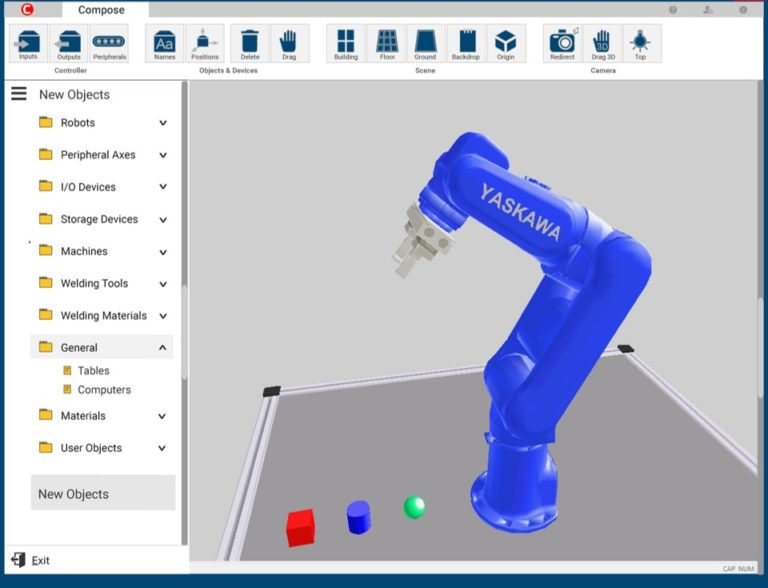
\includegraphics[width=13cm]{figures/Robocell-768x588-1.jpg}
\caption{Software Robocell}
\label{fig:robocell}
\end{figure}

En la figura ~\ref{fig:robocell} se presenta la interfaz que ofrece la empresa Intelitek, esta interfaz como tal no es util, debido que el software fue desarrollado para tener una conexión al programa Scorbase.
\clearpage 

\begin{figure}[h]
\centering
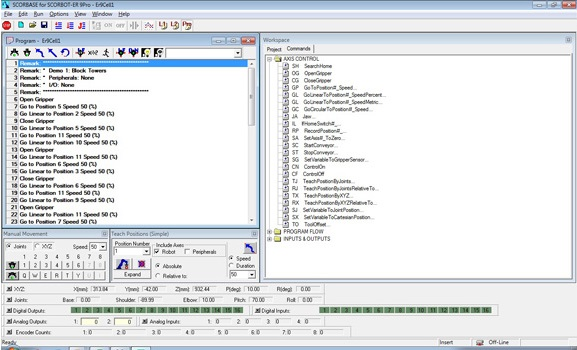
\includegraphics[width=13cm]{figures/eL_RBTC_P_ScorbaseControllerUSBPro_644x350.jpg}
\caption{Software Scorbase}
\label{fig:scorbase}
\end{figure}

En la figura ~\ref{fig:scorbase} se muestra el programa Scorbase, el cual tiene como finalidad programar y operar a los brazos robóticos, además de ofrecer soporte e integración a componentes externos, por ejemplo para realizar monitoreo o cintas transportadoras.

Este programa fue creado especialmente para la operación de maquinaria física, por lo cual carece de una opción de poder visualizar el brazo robótico en uso.

\clearpage
\begin{figure}[h]
\centering
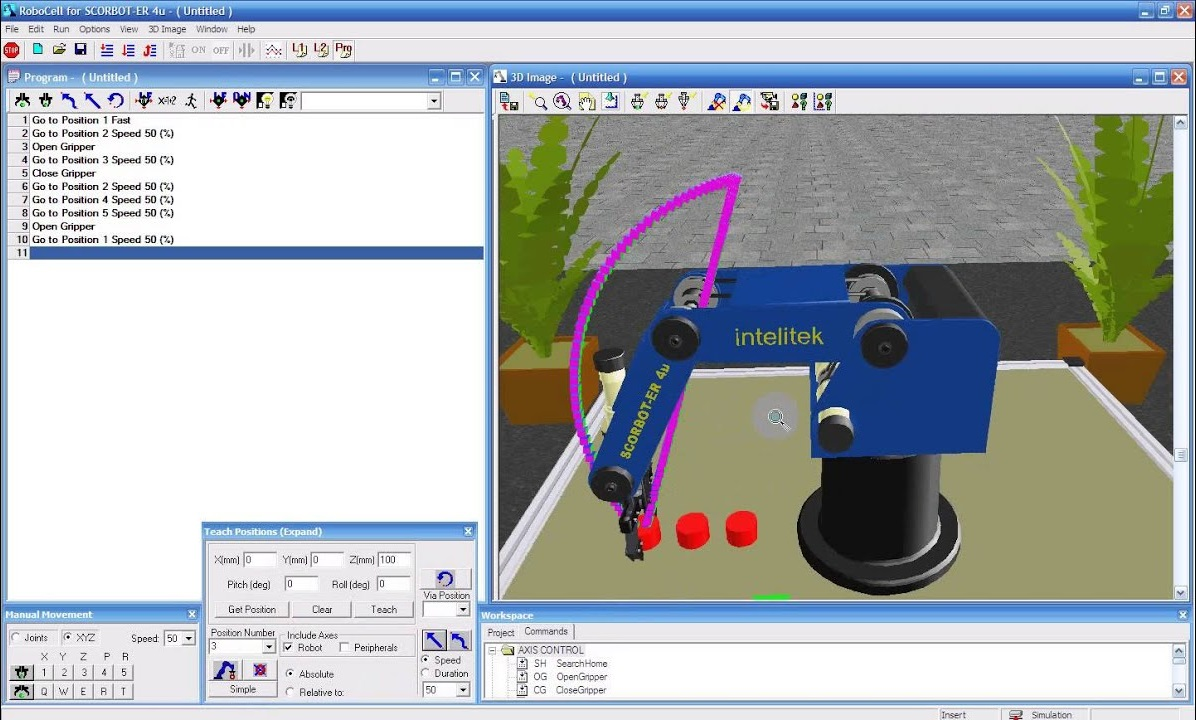
\includegraphics[width=13cm]{figures/robocell scorbase.jpg}
\caption{Software Robocell y Scorbase}
\label{fig:robobase}
\end{figure}

En la figura ~\ref{fig:robobase} se presenta ambos programas funcionando en conjunto,

\subsection{Robots Personales}

\begin{figure}[h]
\centering
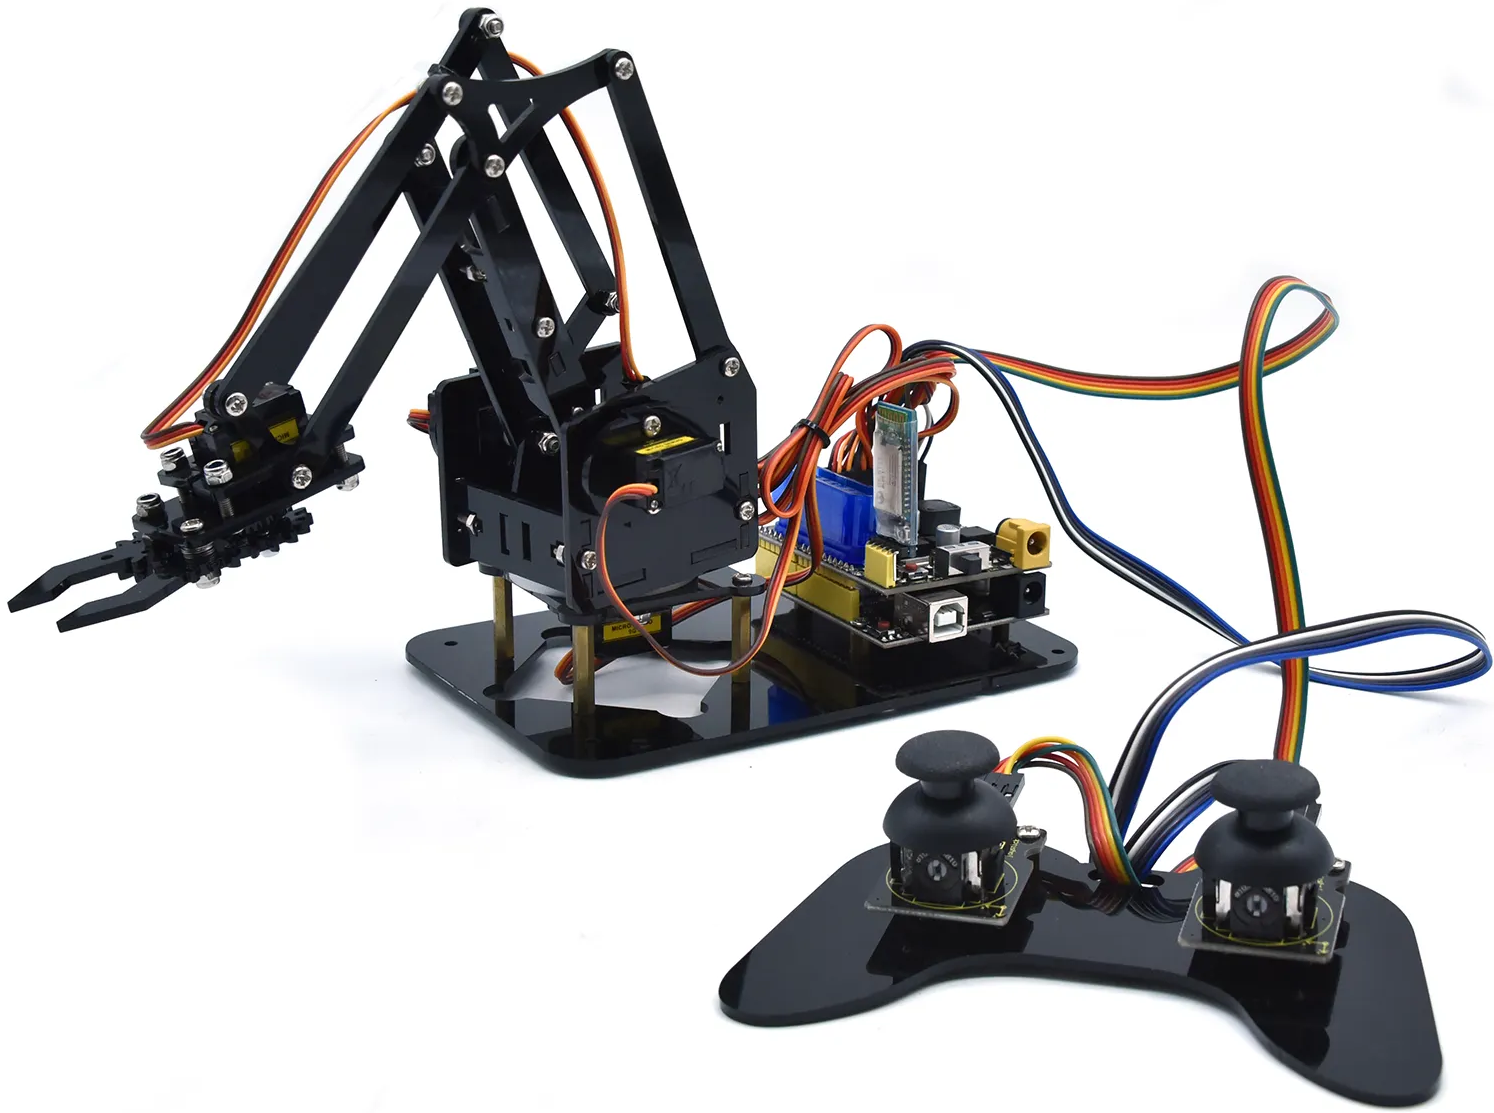
\includegraphics[width=13cm]{figures/Brazo robotico.png}
\caption{Robot Arduino}
\label{fig:robotarduino}
\end{figure}

En la figura 
\chapter{Definición de la institución} En el presente capitulo se presenta la institución y el problema que se aborda en el proyecto.

\section{Descripción de la institución}
\begin{itemize}
\item Nombre: Laboratorio de Sistemas Automatizados de Producción
\item Dirección: Avenida Collao 1202, Concepción, Chile
\item Encargado: Luis Vera
\item Rubro: Automatización
\item Teléfono: (41) 311 1137
\item Descripción: Laboratorio de ensayos para el desarrollo de disciplinas en el ámbito de la Automatización Industrial, Tecnologías Avanzadas de Manufactura, Gestión de la Producción, Robótica, Control Numérico y Visión por Computador.
\end{itemize}

\begin{figure}[ht]
\centering
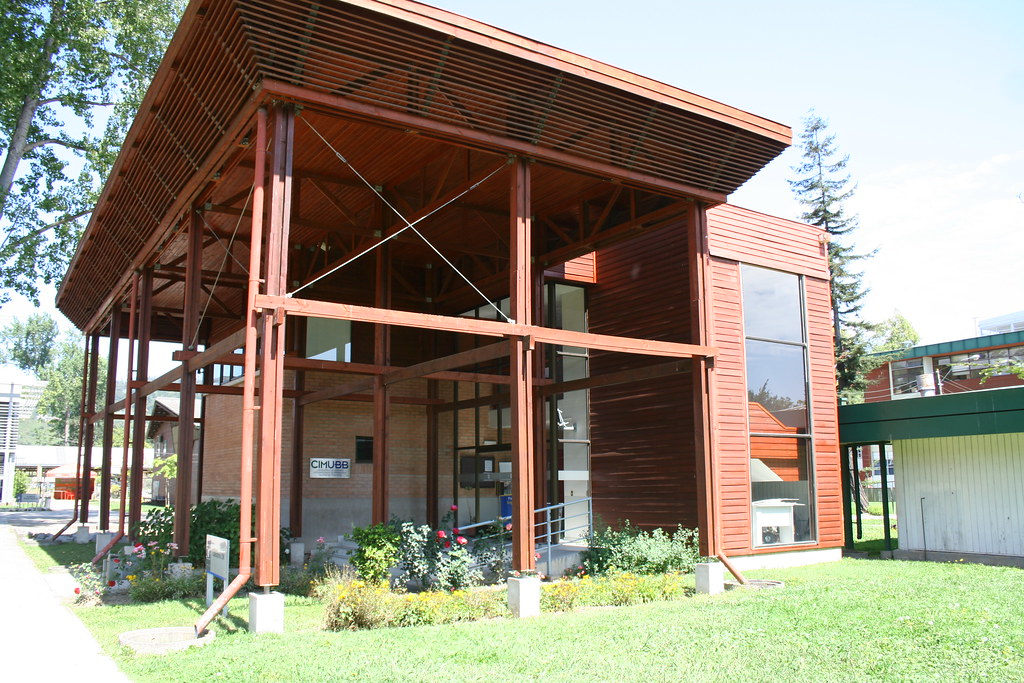
\includegraphics[width=13cm, height=6.8cm]{figures/cimubbfuera.jpg}
\caption{Edificio CIMUBB}
\label{fig:cimubbfuera}
\end{figure}

\clearpage
\section{Descripción del área de estudio}
La presente tesis tiene como objetivo principal abordar el área de estudio relacionada al laboratorio CIMUBB, el cual, por diversas razones, se puede no contar con acceso a este para realizar demostraciones prácticas. La limitación de acceso al laboratorio físico impide brindar una enseñanza completa y práctica a los estudiantes, ya que gran parte del aprendizaje depende de la interacción directa con la maquinaria y los experimentos que se encuentran en su interior.

Con el fin de superar esta limitación, se propone desarrollar un software de simulación que permita a los estudiantes experimentar y aprender de manera virtual dentro del entorno del laboratorio. El software de simulación debe recrear fielmente los equipos, las configuraciones y las condiciones experimentales presentes en el laboratorio real, brindando una experiencia inmersiva y cercana a la realidad.

La simulación se desarrolló utilizando tecnologías de vanguardia y siguiendo los estándares y protocolos establecidos en el campo de estudio correspondiente. Se diseñó una interfaz intuitiva y amigable para facilitar la interacción de los usuarios con los diferentes elementos del laboratorio virtual, permitiéndoles realizar experimentos, ajustar parámetros, recopilar datos y observar los resultados de sus acciones.

La creación de este software de simulación tiene como objetivo principal proporcionar una alternativa efectiva y accesible para la enseñanza y el aprendizaje en ausencia del acceso físico al laboratorio. De esta manera, se busca brindar a los estudiantes una plataforma que les permita adquirir conocimientos prácticos, desarrollar habilidades experimentales y comprender los conceptos teóricos en un entorno virtual seguro y controlado.

Se espera que esta iniciativa proporcione una solución innovadora que amplíe las posibilidades de enseñanza en el área de estudio, permitiendo a los educadores complementar las clases teóricas con experiencias prácticas simuladas. Además, se busca fomentar la autonomía y la experimentación activa por parte de los estudiantes, promoviendo el descubrimiento y la resolución de problemas dentro del contexto del laboratorio virtual.

En resumen, esta investigación se enfoca en el desarrollo de un software de simulación de laboratorio para superar la limitación de acceso físico, permitiendo así una enseñanza práctica y completa en el área de estudio correspondiente. Se espera que esta solución contribuya significativamente a la formación académica y profesional de los estudiantes, brindándoles una herramienta virtual valiosa y efectiva para su aprendizaje y desarrollo.

\clearpage

\section{Descripción de la problemática}
A los comienzos de la pandemia, el profesor encargado del laboratorio CIMUBB, Luis Vera, comienza a notar una necesidad para sus alumnos, una necesidad que siempre estuvo presente pero, para en esa fecha, nunca había sido tan clara ni tan vital como llegó a ser.

\begin{figure}[ht]
\centering
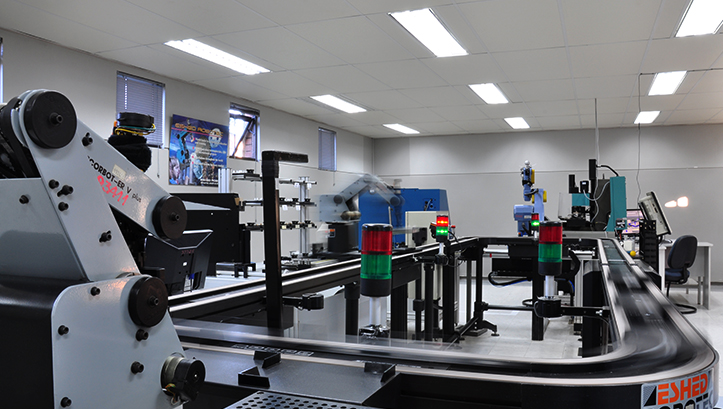
\includegraphics[width=13cm, height=6.1cm]{figures/cimubb.jpg}
\caption{Laboratorio CIMUBB}
\label{fig:cimubb}
\end{figure}

En la Figura ~\ref{fig:cimubb} se muestra una imagen del laboratorio CIMUBB, en el cual se llevan a cabo la entrega del conocimiento sobre la automatización, para la problemática del proyecto se enfoca en los brazos robóticos SCORBOT, los cuales son tres, siendo dos modelos diferentes.

\begin{figure}[ht]
\centering
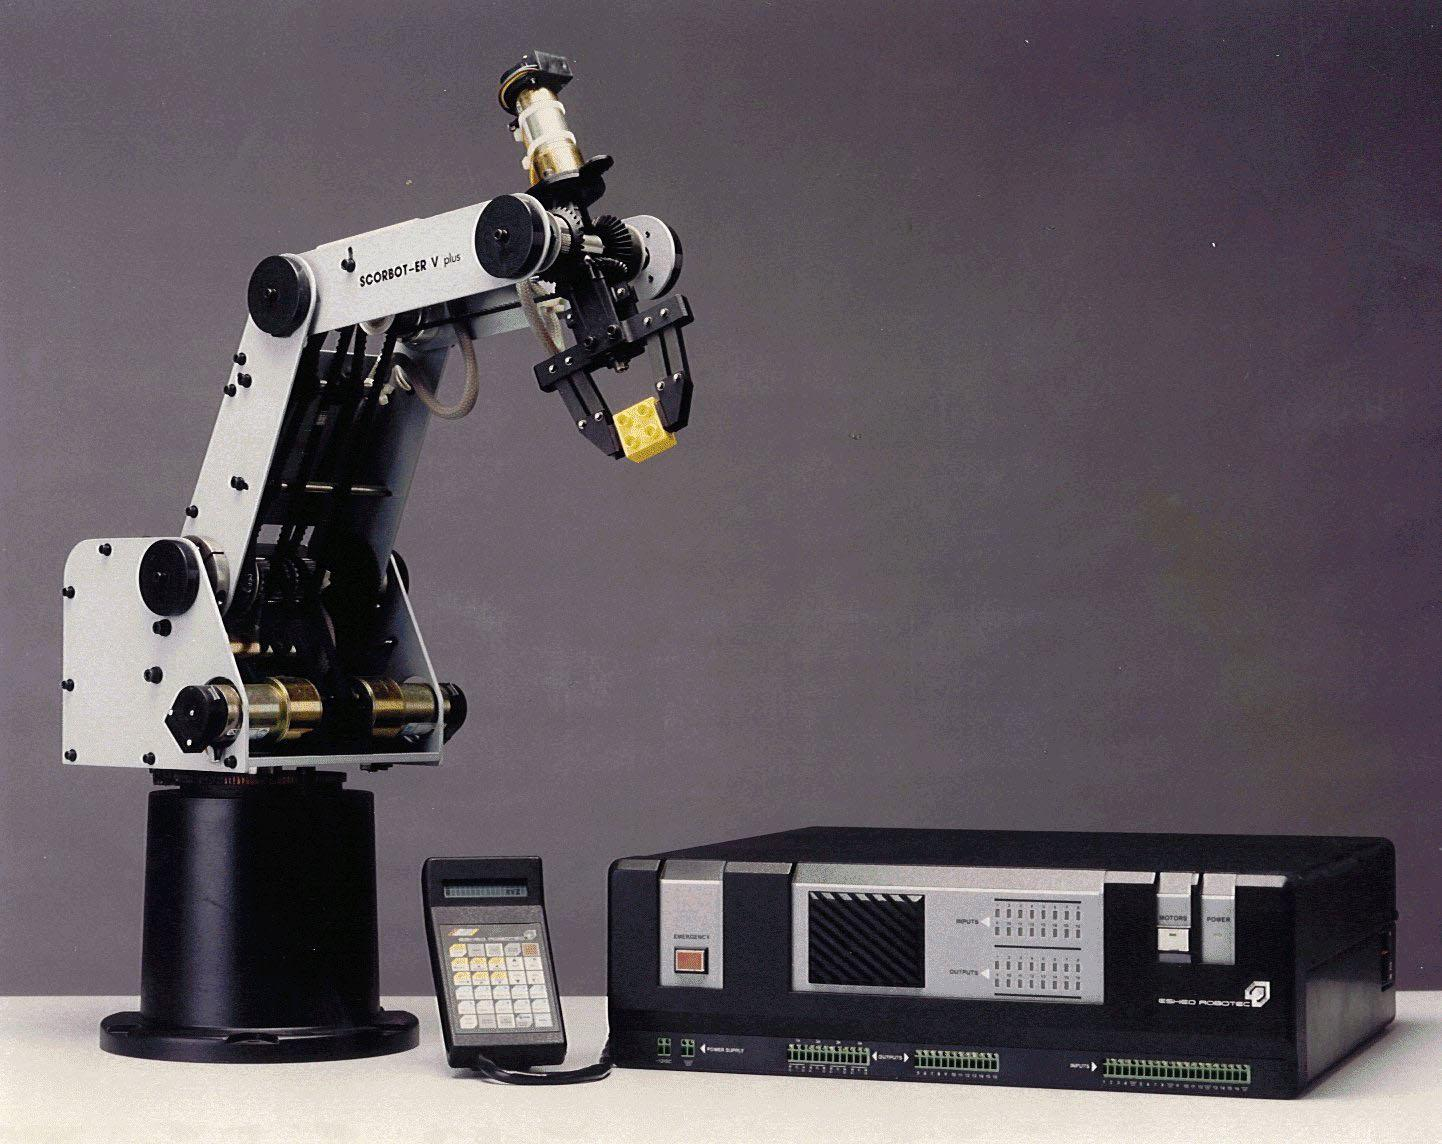
\includegraphics[width=13cm, height=6.1cm]{figures/scor5p.jpg}
\caption{SCORBOT ER V Plus}
\label{fig:scor5p}
\end{figure}

 En la Figura ~\ref{fig:scor5p} se presenta el brazo robótico SCORBOT ER V Plus, es un brazo de antigua generación, teniendo cinco ejes de movimiento para el brazo robótico estático y seis ejes para el que posee una cinta de movimiento lineal.

\clearpage

\begin{figure}[ht]
\centering
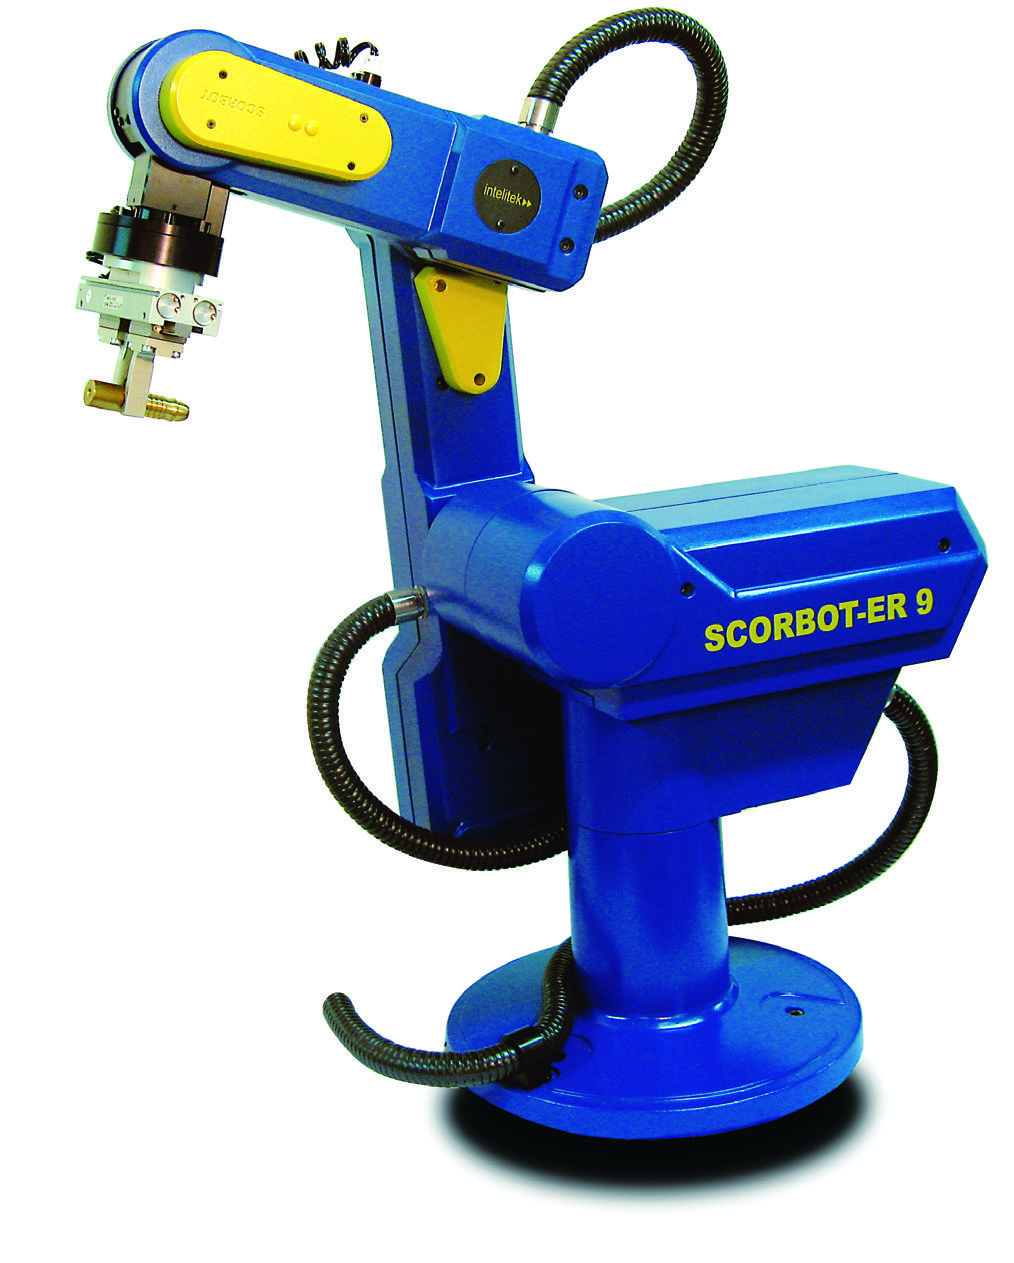
\includegraphics[width=13cm, height=12.5cm]{figures/scor9.jpg}
\caption{SCORBOT ER IX}
\label{fig:scor9}
\end{figure}

En la Figura ~\ref{fig:scor9} se presenta el brazo robótico SCORBOT ER IX, es una versión mejorada, la cual posee siete ejes de movimiento.

El laboratorio CIMUBB no cuenta con un entorno virtual, lo que dificulta significativamente el aprendizaje y la manipulación de los brazos robóticos SCORBOT cuando los estudiantes no pueden acceder físicamente al edificio. La falta de un entorno virtual restringe el acceso de los alumnos a prácticas y experimentos con los brazos robóticos, especialmente durante situaciones como cuarentenas, cortes de luz u otras fallas que requieren la presencia física de un supervisor o profesor.

La falta de acceso a un entorno virtual también limita la flexibilidad y disponibilidad para los estudiantes que deseen aprender sobre sistemas automatizados y brazos robóticos fuera de los horarios de clases regulares. Si el profesor no tiene acceso físico al laboratorio en un momento dado, los estudiantes se ven obligados a esperar hasta que el profesor pueda estar presente nuevamente en el lugar para realizar cualquier actividad relacionada con los brazos robóticos.
\chapter{Definición proyecto} En este capitulo se detallan los objetivos, la metodología que se utiliza, y las tecnologías en la cual se apoya.

\section{Objetivos del proyecto}

\subsection{Objetivo General}
Desarrollar una aplicación en Unity que permita simular el laboratorio
del CIMUBB, con la cual los estudiantes puedan probar el funcionamiento de los
brazos robóticos SCORBOT ER V Plus y el brazo robótico SCORBOT ER IX , intentando replicar con el mayor detalle posible
las estaciones de los brazos en el laboratorio.

\subsection{Objetivos Específicos}
\begin{enumerate}[label=\roman*.-]
\item Examinar los desafíos inherentes de la problemática que presenta el laboratorio.
\item Analizar tecnologías y herramientas con el fin de comprender su funcionamiento y utilizarlas de manera eficaz en la resolución del problema.
\item Desarrollar la aplicación.
\end{enumerate}

\subsection{Actividades}
Las actividades desarrolladas en este proyecto son:
\begin{enumerate}[label=\roman*.-]
\item Examinar los desafíos inherentes de la problemática que presenta el laboratorio.
    \begin{enumerate}[label=\arabic*.-]
    \item Investigación sobre los factores que originan la problemática.
    \end{enumerate}
\item Analizar tecnologías y herramientas con el fin de comprender su funcionamiento y utilizarlas de manera eficaz en la resolución del problema.
    \begin{enumerate}[label=\arabic*.-]
    \item Exploración y análisis de diversas herramientas de programación con el propósito de comprender sus características y funcionalidades.
    \item Investigación para evaluar las posibilidades que ofrecen distintas herramientas de programación y determinar cuál es la más adecuada para abordar el proyecto.
    \end{enumerate}
\item Desarrollar la aplicación
    \begin{enumerate}[label=\arabic*.-]
    \item Investigación sobre el laboratorio.
    \item Diseño de entorno y equipamiento.
    \item Desarrollo de código para dar funciones.
    \item Diseño de interfaz gráfica.
    \item Desarrollo de funcionalidad de la interfaz gráfica.
    \end{enumerate}
\end{enumerate}

\section{Ambiente de ingeniería de software}
\subsection{Metodología de Desarrollo}
La metodología de desarrollo a utilizar a lo largo del proyecto es incremental \cite{Incremental}, pues se debe a que facilita al desarrollo del proyecto y saber si se encuentra por un buen camino, debido a que se le presenta cada incremento al cliente y obtener una retroalimentación del mismo.

\subsection{Tecnologías}
\begin{table}[h!]
\begin{center}
\begin{tabular}{ m{0.15\linewidth} m{0.12\linewidth} m{0.65\linewidth} }
\noalign{\hrule height 2pt}
Nombre & Logo & Descripción \\ 
\noalign{\hrule height 2pt}

C\# & 

\includegraphics[height=0.12\textwidth]{figures/c.png} & 
C\# es uno de los lenguajes de programación diseñados para la infraestructura de lenguaje común . Su sintaxis básica deriva de C / C++ y utiliza el modelo de objetos de la plataforma .NET, similar al de Java, aunque incluye mejoras derivadas de otros lenguajes.
 \\
\hline
\end{tabular}
\caption{Tecnologías}
\end{center}
\end{table}

\clearpage
\subsection{Herramientas de apoyo}
\begin{table}[h!]
\begin{center}
\begin{tabular}{ m{0.15\linewidth} m{0.12\linewidth} m{0.65\linewidth} }
\noalign{\hrule height 2pt}
Nombre & Logo & Descripción \\ 
\noalign{\hrule height 2pt}

Unity & 

\includegraphics[height=0.12\textwidth]{figures/Unity.png} & 
Unity es un motor de desarrollo en tiempo real que te permite crear experiencias interactivas en el Editor de Unity que se utiliza para la creación de videojuegos. Estos se pueden publicar en diversas plataformas como PC, videoconsolas, móviles, etc. Gracias a su flexibilidad es una herramienta que también se usa en diferentes industrias como arquitectura, ingeniería, automotriz y de entretenimiento.
 \\
\hline

Blender & 

\includegraphics[height=0.09\textwidth]{figures/Blender.png} & 
Blender es un programa informático multiplataforma, dedicado especialmente al modelado, iluminación, renderizado, la animación y creación de gráficos tridimensionales. También de composición digital utilizando la técnica procesal de nodos, edición de vídeo, escultura (incluye topología dinámica) y pintura digital.
\\
\hline

Visual Studio Code & 

\includegraphics[height=0.1\textwidth]{figures/VSC.png} & 
Es un editor de código fuente desarrollado por Microsoft para Windows, Linux y macOS. Incluye soporte para la depuración, control integrado de Git, resaltado de sintaxis, finalización inteligente de código, fragmentos y refactorización de código.
\\ 
\hline

GitHub & 

\includegraphics[height=0.1\textwidth]{figures/GitHub.png} & 
Es un servicio en la nube que ayuda a los desarrolladores a almacenar y administrar su código, al igual que llevar un registro y control de cualquier cambio sobre este código.
\\ 
\hline

\end{tabular}
\caption{Herramientas de apoyo}
\end{center}
\end{table}

\chapter{Especificación de requerimientos de software} En el siguiente capitulo se presentan los requerimientos de la aplicación.

\section{Alcances}
El alcance de la simulación abarca la recreación de los brazos Scorbot y otros componentes y maquinarias presentes en el laboratorio, aunque estos últimos no serán funcionales. Entre estos elementos se incluye una cinta transportadora y un objeto específico que el brazo Scorbot podrá tomar y manipular.

La simulación se centra en replicar el comportamiento y las características de los brazos Scorbot de manera precisa, garantizando un rango de movimiento y una capacidad de manipulación de objetos lo más realista posible. Además, se incluye una representación visual detallada de los brazos Scorbot y de los demás componentes y maquinarias presentes en el laboratorio.

El brazo róbotico Scorbot puede realizar su movimiento en modo Joints, el cual hace girar en función de los motores. Por otra parte, el movimiento en modo XYZ no esta disponible debido a fallos de diseño del modelado del robot. El brazo tampoco es capaz de realizar movimientos guardados, sin embargo en el código se esta planteado la lógica de esta.

La cinta transportadora esta disponible en la simulación, pero no funciona como en el entorno físico. Su presencia permite a los estudiantes experimentar con la interacción del brazo Scorbot en relación con la transferencia de objetos a lo largo de la cinta, aunque su movimiento y operación real no estarán habilitados del todo. Esto debido a darle mas importancia al brazo como tal, sin embargo, se implemento un código rustico, el cual sirve pero no esta pulido y tiene varias fallas.

Asimismo, se proporcionarun objeto específico en la simulación que el brazo Scorbot podrá tomar y manipular. Esto permite a los usuarios practicar las habilidades de agarre y manipulación del brazo, familiarizándose con los comandos y las técnicas necesarias para realizar estas tareas.

Es importante tener en cuenta que, aunque los componentes y otras maquinarias estarán presentes en la simulación, su funcionalidad real no estará activa. El enfoque principal será brindar a los estudiantes una experiencia interactiva y visualmente representativa del entorno del laboratorio, centrándose en la operación y el uso del brazo Scorbot.

\section{Objetivo del software}
El objetivo del software de simulación desarrollado es proporcionar una herramienta virtual que permita a los estudiantes experimentar, aprender y practicar el funcionamiento de los brazos Scorbot y otros componentes del laboratorio, en ausencia del acceso físico al mismo.

Los principales objetivos del software de simulación son:
\begin{enumerate}[label=\arabic*.-]
\item Brindar una experiencia realista: El software se diseñará con el objetivo de recrear de manera precisa y realista el comportamiento y las capacidades de los brazos Scorbot, así como otros componentes y maquinarias presentes en el laboratorio. Se buscará proporcionar una representación visual y funcionalidad detalladas, para que los estudiantes puedan interactuar con ellos de manera similar a como lo harían en el entorno físico.
\item Facilitar la práctica y el aprendizaje: El software permitirá a los estudiantes practicar y adquirir habilidades en el uso y manejo de los brazos Scorbot, así como explorar la interacción con otros componentes del laboratorio. Los usuarios podrán realizar diferentes tareas y experimentos, ajustar parámetros y recopilar datos, todo dentro de un entorno virtual controlado y seguro.
\item Fomentar la comprensión teórica y práctica: El software de simulación ayudará a los estudiantes a comprender los conceptos teóricos relacionados con el funcionamiento de los brazos Scorbot y su aplicación en diferentes situaciones. Podrán experimentar directamente los efectos de las acciones realizadas y observar los resultados de sus interacciones, lo que fortalecerá su comprensión de los principios subyacentes.
\item Superar limitaciones de acceso: Al proporcionar una alternativa virtual al laboratorio físico, el software de simulación permitirá a los estudiantes acceder al aprendizaje práctico y experiencial en cualquier momento y lugar, sin restricciones de horarios o limitaciones de espacio físico. Esto ampliará las oportunidades de aprendizaje y brindará una opción adicional para aquellos que no tienen acceso directo al laboratorio.
\end{enumerate}
\section{Descripción global del producto}
\subsection{Interfaz de usuario}
La interfaz de usuario es diseñada con un enfoque en la amigabilidad y familiaridad para minimizar la resistencia al cambio y maximizar la adaptabilidad. Al crear una interfaz que los usuarios encuentren intuitiva, se facilita su aceptación y comodidad al utilizar el software. Además, la adaptabilidad es crucial para garantizar que la interfaz funcione de manera eficiente en diferentes contextos y dispositivos, permitiendo a los usuarios acceder y utilizar el programa de manera óptima en diversas situaciones. Un diseño cuidadoso y una atención especial a la experiencia del usuario pueden fomentar una transición más fluida y exitosa hacia el software.
\subsection{Interfaz de hardware}
En el contexto de computadoras, las interfaces de hardware típicas son el teclado y el ratón para la entrada de datos, y el monitor para la salida visual. Mientras que en el caso de teléfonos y tabletas, las interfaces de hardware se basan en pantallas táctiles, que permiten a los usuarios interactuar directamente con el dispositivo mediante toques y gestos en la pantalla.
\subsection{Interfaz software}
El programa no requiere la instalación de software externo adicional, ya que funciona directamente en sistemas operativos como Windows, Linux o Android. Esto implica que los usuarios pueden ejecutar el programa sin necesidad de instalar bibliotecas o programas adicionales, lo que simplifica su implementación y uso en diferentes plataformas. La compatibilidad con estos sistemas operativos amplía la accesibilidad del programa a una variedad de dispositivos y entornos, facilitando su distribución y adopción.
\section{Requerimientos específicos}

\subsection{Requerimientos funcionales del sistema}

Se presentan los requerimientos funcionales de la aplicación, donde se destaca las características que tiene.

\begin{table}[h!]
\begin{center}
\begin{tabular}{ | m{0.09\linewidth} | m{0.17\linewidth} | m{0.66\linewidth} | }
\noalign{\hrule height 2pt}
ID & Nombre & Descripción \\ 
\noalign{\hrule height 2pt}

RF-01 & 
Controlar el brazo robótico & 
La aplicación debe permitir al usuario hacer uso del brazo robótico
 \\
\hline

RF-02 & 
Controlar botonera & 
La aplicación debe permitir al usuario hacer uso de la botonera del brazo robótico
 \\
\hline

\end{tabular}
\caption{Requerimientos funcionales}
\end{center}
\end{table}
\chapter{Factibilidad} En el capítulo actual se mostrará la factibilidad que tiene el proyecto de ser realizado.

\section{Factibilidad Técnica}

Requerimiento para el desarrollo:
\begin{table}[h!]
\centering
\begin{tabular}{ | p{0.13\linewidth} | p{0.2\linewidth} | p{0.25\linewidth} | p{0.3\linewidth} |}
\noalign{\hrule height 2pt}
Requisitos

mínimos & Windows & macOS & Linux \\ 
\noalign{\hrule height 2pt}

Versión 

sistema 

operativo & 
Windows 7 

(Service Pack 1+),

Windows 10 y 

Windows 11 & 
High Sierra 10.13+ &
Ubuntu 20.04, Ubuntu 18.04, y CentOS 7
 \\
\hline

Procesador & 
Arquitectura x86 o

x64 con soporte de

instrucción SSE2 & 
Arquitectura x64 con

soporte de instrucción

SSE2 para CPU Intel,

Apple M1 o superior

para CPU Apple & 
Arquitectura x64 con soporte

de instrucción SSE2
 \\
\hline

API Gráfico & 
GPU compatible

con DirectX 

versión 10, 11 o 12 & 
GPU Intel, AMD o Apple compatible con Metal &
GPU compatible con

OpenGL 3.2+ o Vulkan
 \\
\hline

\end{tabular}
\caption{Requerimientos de desarrollo en computadores}
\end{table}

\clearpage
Factibilidad Técnica para Desarrollo Unity en un Notebook con Ryzen 7 5700U, 16GB RAM y Ubuntu:

\begin{enumerate}[label=\arabic*.]
\item \textbf{Compatibilidad con Sistema Operativo:}
\begin{itemize}
\item \textbf{Factible:} El sistema operativo Ubuntu 20.04 es compatible con los requisitos mínimos para el desarrollo en Unity. Además, la arquitectura x64 del procesador Ryzen 7 5700U es compatible.
\end{itemize}

\item \textbf{Procesador:}
\begin{itemize}
\item \textbf{Factible:} El Ryzen 7 5700U es un procesador x64 con soporte para instrucciones SSE2, cumpliendo así con los requisitos mínimos de Unity.
\end{itemize}

\item \textbf{API Gráfico:}
\begin{itemize}
\item \textbf{Factible:} Ubuntu 20.04 es compatible con OpenGL 3.2+, y el Ryzen 7 5700U tiene una GPU integrada que es capaz de soportar esta versión de OpenGL.
\end{itemize}

\item \textbf{Memoria RAM:}
\begin{itemize}
\item \textbf{Factible:} Con 16GB de RAM, el sistema cumple con los requisitos mínimos, lo que proporcionará suficiente memoria para el desarrollo en Unity.
\end{itemize}

\item \textbf{Conexión a Internet:}
\begin{itemize}
\item \textbf{Factible:} Dado que algunos recursos y actualizaciones de Unity pueden requerir una conexión a Internet, es recomendable tener acceso a una conexión estable.
\end{itemize}

\item \textbf{Espacio en Disco:}
\begin{itemize}
\item \textbf{Factible:} Con 400GB disponibles en un disco de 500GB, cumples con el requisito mínimo de 15GB libres que necesita Unity. Es completamente factible.
\end{itemize}

\item \textbf{Compatibilidad con Controladores Gráficos:}
\begin{itemize}
\item \textbf{Factible:} Los controladores gráficos usados en Vulkan son mesa v23, siendo así compatibles con Unity.
\end{itemize}
\end{enumerate}

En resumen, después de analizar todos los aspectos técnicos, se determina que el proyecto es factible. Las especificaciones del notebook cumplen con los requisitos mínimos de Unity, y los recursos necesarios están disponibles para el desarrollo sin necesidad de hardware adicional significativo.

\clearpage

\section{Factibilidad Operativa}

\begin{enumerate}
    \item \textbf{Recursos Humanos:}
    Como desarrollador del simulador con experiencia en programación y Unity, los recursos humanos necesarios ya están disponibles internamente. La capacitación para los usuarios se limita a conocimientos básicos sobre el uso de un dispositivo.

    \item \textbf{Recursos Físicos:}
    Con los datos que entrega la cámara de diputados en 2022\cite{InformeCamara}, se puede asumir que de los 3.89 millones de usuarios de internet fija en la zona residencial, debe tener al menos un computador, por lo cual se dice que al menos 3.89 millones de personas serian potenciales usuarios.

    \item \textbf{Tecnología y Sistemas de Información:}
    La restricción de hardware para Unity (computadoras desde 2012 y celulares Android desde 2011) se considera aceptable y probablemente cubra una gran parte de los dispositivos en uso actualmente.

    \item \textbf{Cumplimiento Normativo:}
    Dado que el simulador no almacena datos, no hay problemas de privacidad y seguridad que considerar.

    \item \textbf{Experiencia del Usuario:}
    La interfaz del simulador se diseñó de manera simple para facilitar su uso.

\end{enumerate}

La factibilidad operativa del simulador de brazos robóticos en Unity es sólida. Con recursos humanos disponibles, un amplio alcance potencial, requisitos tecnológicos razonables y la ausencia de procesos operativos complejos, el simulador parece ser una herramienta eficiente y accesible para entornos educativos.

\section{Impacto Positivo:}

\begin{enumerate}
    \item \textbf{Experimentación sin riesgos:} Los entornos virtuales en Unity permiten a los investigadores y estudiantes realizar experimentos y pruebas sin riesgos ni costos asociados con el mundo real. Esto es especialmente útil en campos como la investigación médica, química o física, donde los experimentos pueden ser costosos o peligrosos.
    
    \item \textbf{Acceso universal:} Los entornos virtuales pueden ser accesibles desde cualquier lugar, lo que facilita la colaboración y el acceso a recursos educativos o de investigación para personas de todo el mundo.
    
    \item \textbf{Aprendizaje interactivo:} Para fines educativos, un entorno virtual en Unity puede proporcionar una experiencia de aprendizaje más interactiva y atractiva. Puede mejorar la comprensión de conceptos complejos al permitir a los estudiantes interactuar directamente con modelos y simulaciones.
    
    \item \textbf{Personalización:} Los entornos virtuales pueden adaptarse para satisfacer las necesidades específicas del laboratorio o del programa educativo. Esto permite una mayor personalización y adaptabilidad a diferentes objetivos de investigación o de aprendizaje.
    
    \item \textbf{Reducción de costos:} Al utilizar entornos virtuales, se pueden reducir los costos asociados con la compra de equipos especializados, materiales y mantenimiento de laboratorios físicos.
\end{enumerate}

\section{Impacto Negativo:}

\begin{enumerate}
    \item \textbf{Limitaciones de simulación:} Aunque los entornos virtuales son poderosos, no siempre pueden replicar completamente la complejidad del mundo real. Pueden haber limitaciones en la simulación de ciertos fenómenos o situaciones.
    
    \item \textbf{Requisitos técnicos:} La implementación y el uso de entornos virtuales en Unity pueden requerir habilidades técnicas y recursos significativos. Esto podría ser un desafío para algunos laboratorios que no tienen acceso a personal técnico o hardware adecuado.
    
    \item \textbf{Aislamiento:} Dependiendo de cómo se implemente, la tecnología virtual puede llevar al aislamiento del mundo real. Los estudiantes o investigadores pueden perder la experiencia táctil y la interacción directa con los objetos y fenómenos que están estudiando.
    
\end{enumerate}

\section{Factibilidad Económica}

\textbf{Costo de personal}

Dado que el proyecto de tesis se desarrolla dentro de un entorno académico y no implica la contratación ni la compensación económica adicional para el personal involucrado, no se incluye un ítem de gasto en recursos humanos. La naturaleza educativa y formativa del proyecto permite que los participantes, principalmente los estudiantes responsables de la tesis, contribuyan sin generar desembolsos económicos adicionales para el proyecto. La ausencia de este gasto fortalece la viabilidad económica del proyecto en el ámbito académico.

\textbf{Costo de desarrollo}

El gasto asociado al desarrollo del proyecto es asumido por un estudiante en proceso de titulación, lo que implica que el costo directo asignado al estudiante es de 0 CLP. Sin embargo, con el propósito de realizar una evaluación económica, se emplea el promedio de la tarifa por hora de un ingeniero civil informático, fijada en 6000 pesos chilenos. Esta estimación se utiliza como una medida representativa del valor del tiempo y la contribución del estudiante al proyecto, a pesar de que no se traduzca en un desembolso financiero directo en este contexto académico.

\begin{table}[ht]
    \centering
    \begin{tabular}{|l|c|c|c|c|}
        \hline
        \textbf{Fase} & \textbf{Porcentaje} & \textbf{Horas} & \textbf{Costo por Hora} & \textbf{Costo Total} \\
        \hline
        Diseño & 10\% & 58.5 & 6000 & 351,000 \\
        \hline
        Desarrollo & 45\% & 263.25 & 6000 & 1,579,500 \\
        \hline
        Implementación & 20\% & 117 & 6000 & 702,000 \\
        \hline
        Pruebas & 15\% & 87.75 & 6000 & 526,500 \\
        \hline
        \multicolumn{4}{|r|}{\textbf{Costo Total de Desarrollo}} & \textbf{3,159,000} CLP \\
        \hline
    \end{tabular}
    \caption{Costo de Desarrollo del Proyecto en Unity}
    \label{tab:costo-desarrollo}
\end{table}


\textbf{Costo de hardware}
La ausencia de inversión en hardware se justifica por el hecho de que la aplicación se ejecutará de manera eficiente en los computadores personales de los estudiantes, eliminando así la necesidad de adquirir equipamiento adicional. Este enfoque estratégico garantiza que los recursos tecnológicos existentes sean plenamente utilizados, minimizando cualquier requerimiento financiero relacionado con la infraestructura de hardware del proyecto.

\begin{table}[ht]
    \centering
    \label{tab:financial-evaluation}
    \begin{tabular}{ | p{0.18\linewidth} | c | c | c | c | c | c | }
        \hline
        \textbf{Año} & \textbf{0} & \textbf{1} & \textbf{2} & \textbf{3} & \textbf{4} & \textbf{5} \\
        \hline
        
        Desarrollo & -3,159,000 & - & - & - & - & - \\
        \hline
        Utilidad & - & 165,000 & 330,000 & 495,000 & 660,000 & 825,000 \\
        \hline
        Impuesto & - & 28,050 & 56,100 & 84,150 & 112,200 & 140,250 \\
        \hline
        Utilidad después 
        
        de impuesto & - & 136,950 & 273,900 & 410,850 & 547,800 & 684,750 \\
        \hline
        Utilidad del 
        
        periodo & -3,159,000 & -3,022,050 & -2,748,150 & -2,337,300 & -1,789,500 & -1,104,750 \\
        \hline
    \end{tabular}
    \caption{Evaluación Financiera del Proyecto}
\end{table}

\begin{enumerate}[label=\arabic*.]
    \item \textbf{Desarrollo:} Este campo representa los costos asociados con la fase de desarrollo del proyecto. En el año 0, se muestra el monto de inversión inicial necesario para el desarrollo del proyecto. En el ejemplo proporcionado, este valor es de -3,159,000 CLP, lo que indica un gasto.
    
    \item \textbf{Utilidad:} Representa la ganancia generada por el proyecto en cada año después de la deducción de los costos y gastos, pero antes de impuestos. En este contexto, la "Utilidad" refleja la estimación de reducción de costos asociados con el mantenimiento del brazo robótico. Inicialmente, el costo de mantenimiento es de 165,000 CLP por mes. Gracias a la implementación del software, se estima que la eficiencia aumentará, lo que resultará en la reducción de un mes de mantenimiento por año. Por lo tanto, la "Utilidad" refleja tanto los ahorros en costos de mantenimiento como cualquier otra ganancia generada por el proyecto, sin considerar impuestos en esta etapa del análisis.
    
    \item \textbf{Utilidad del periodo:} Representa la ganancia neta después de impuestos y es el resultado final de restar el impuesto de la utilidad antes de impuestos. Este valor muestra la ganancia neta real que el proyecto genera después de cumplir con las obligaciones tributarias. En el ejemplo, los valores de "Utilidad del periodo" son negativos en los primeros años debido a los costos iniciales y el impacto del impuesto.
\end{enumerate}

\clearpage
\section{Conclusión de la factibilidad}

En conclusión, después de analizar la factibilidad técnica, operativa y económica del proyecto de simulador de brazos robóticos en Unity, se puede afirmar que el proyecto es factible y presenta un potencial impacto positivo en diversas áreas.

Desde el punto de vista técnico, los requisitos de hardware y software necesarios para el desarrollo en Unity son cumplidos por el equipo de desarrollo propuesto, especialmente en el caso del notebook con Ryzen 7 5700U y Ubuntu. Este análisis asegura que la implementación del proyecto no requiera hardware adicional significativo.

En términos operativos, la disponibilidad de recursos humanos, físicos y tecnológicos es sólida. El proyecto cuenta con un desarrollador con experiencia en programación y Unity, y se proyecta un amplio alcance potencial gracias a la cantidad estimada de usuarios de internet fija en la zona residencial.

El impacto positivo del proyecto se refleja en la posibilidad de realizar experimentos sin riesgos, el acceso universal a la herramienta, el aprendizaje interactivo, la personalización según las necesidades y la reducción de costos asociados con laboratorios físicos.

La evaluación económica muestra que, a pesar de los costos iniciales de desarrollo, el proyecto tiene el potencial de generar utilidades a partir del segundo año. La ausencia de costos de personal y hardware adicionales contribuye a la viabilidad económica del proyecto, y el análisis financiero proyecta una utilidad neta positiva en los años subsiguientes.

En resumen, la factibilidad del proyecto se respalda sólidamente en los aspectos técnico, operativo y económico, lo que sugiere que la implementación del simulador de brazos robóticos en Unity es una propuesta viable y prometedora.
\chapter{Análisis} En este capitulo que nos conlleva a analizar los actores que ejecutaran la aplicación, los flujos que esta tendrá.

\section{Interacción del Usuario en la Simulación}
\begin{figure}[h]
\centering
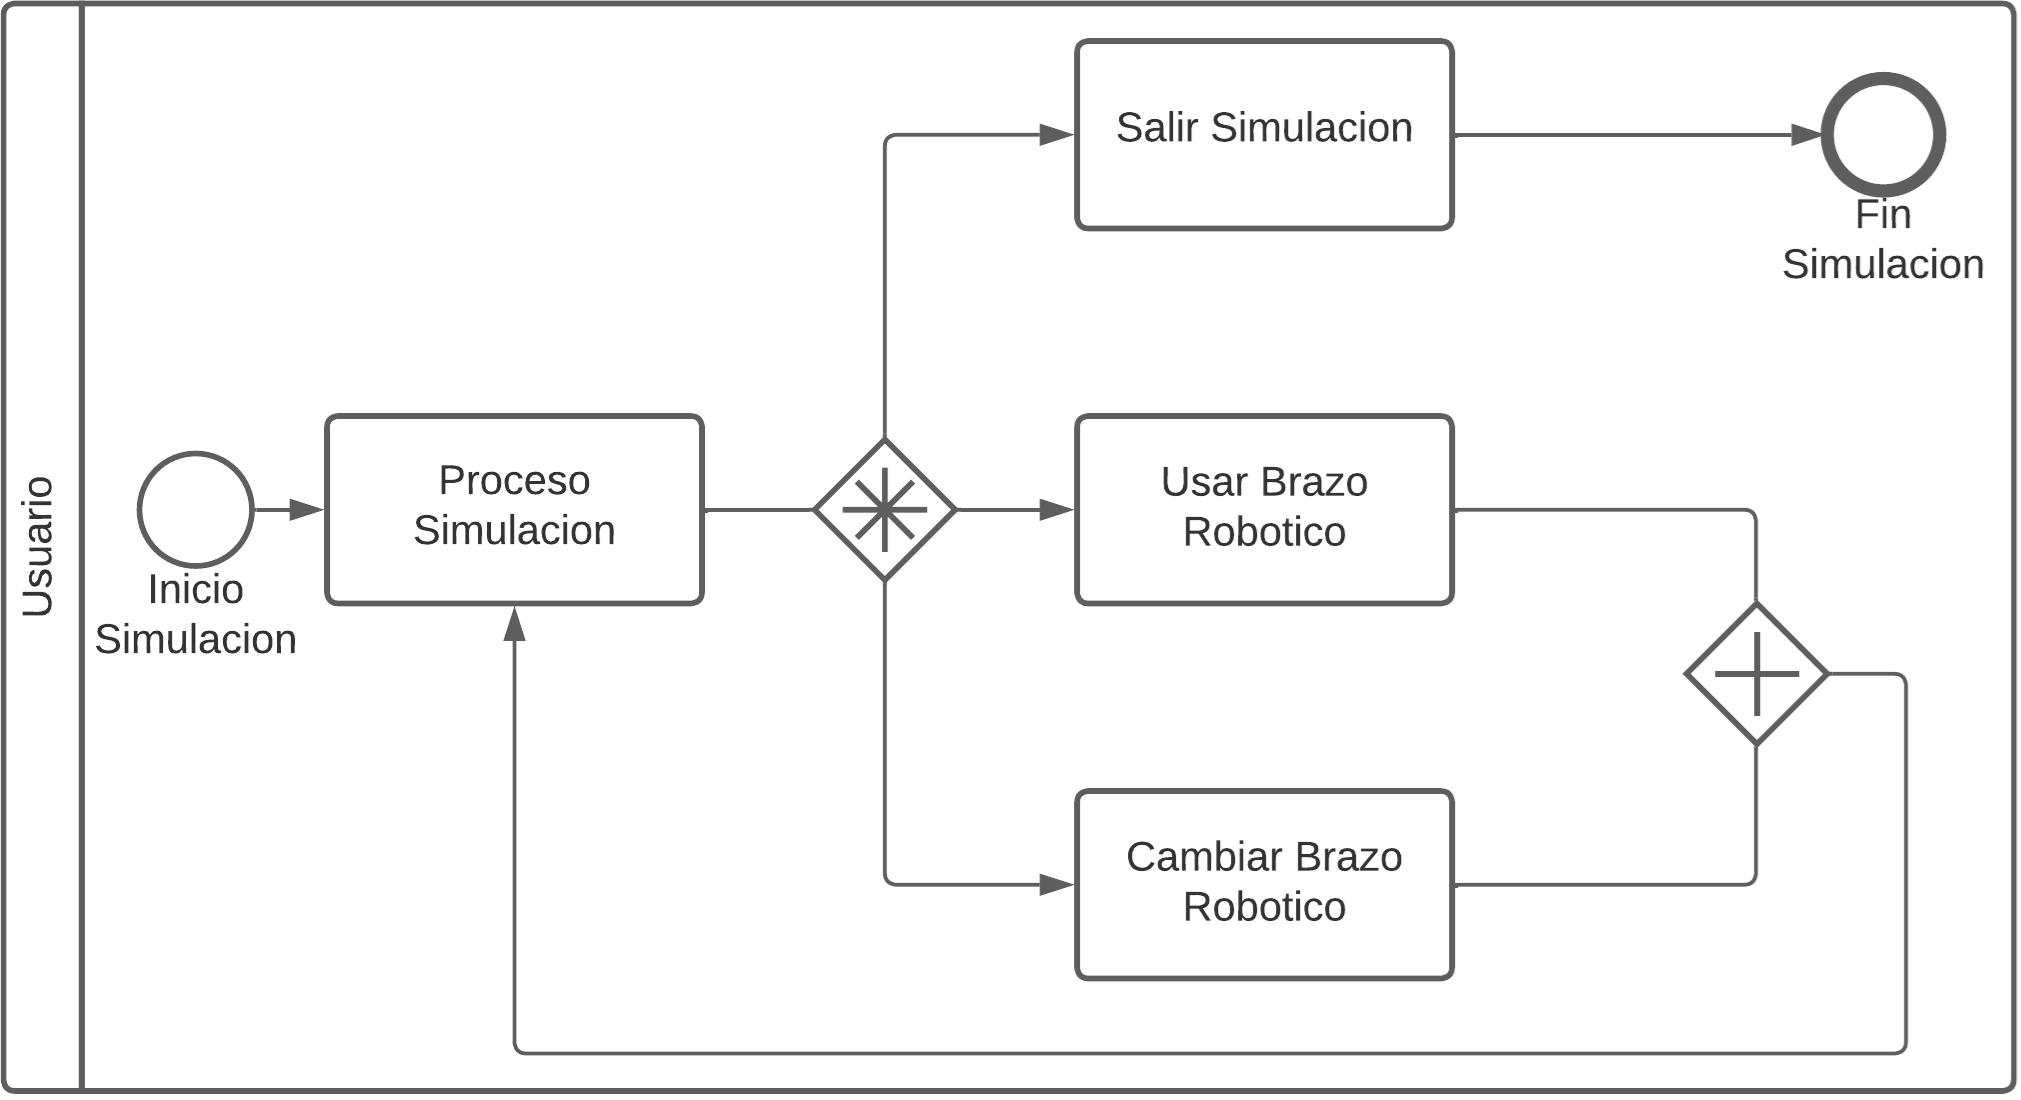
\includegraphics[height=6.83cm]{figures/bpmn.png}
\caption{BPMN de la Interacción}
\label{fig:bpmn}
\end{figure}

En la Figura ~\ref{fig:bpmn} se muestra el proceso de como el usuario interactúa con la simulación, el proceso inicia con el usuario ejecutando la simulación, una vez dentro de esta, el usuario puede elegir entre usar el brazo robótico, cambiar de brazo robótico, con las cuales lo lleva a mantenerse en el proceso de la simulación, por ultimo esta la opción de salir de la simulación que finaliza este proceso

\section{Casos de uso}
\subsection{Actores}
Usuario: Persona que utilizara la aplicación, ya sea estudiante o profesor de la Universidad del Bío-Bío, como también personas externas a esta. El usuario puede utilizar la aplicación completamente.

\subsection{Diagrama de casos de uso y descripción}
Este capítulo destaca los casos de uso del proyecto, ofreciendo una visión rápida de las interacciones que los usuarios pueden realizar.


\textbf{Caso de uso: Uso de Interfaz Principal}
\begin{figure}[h]
\centering
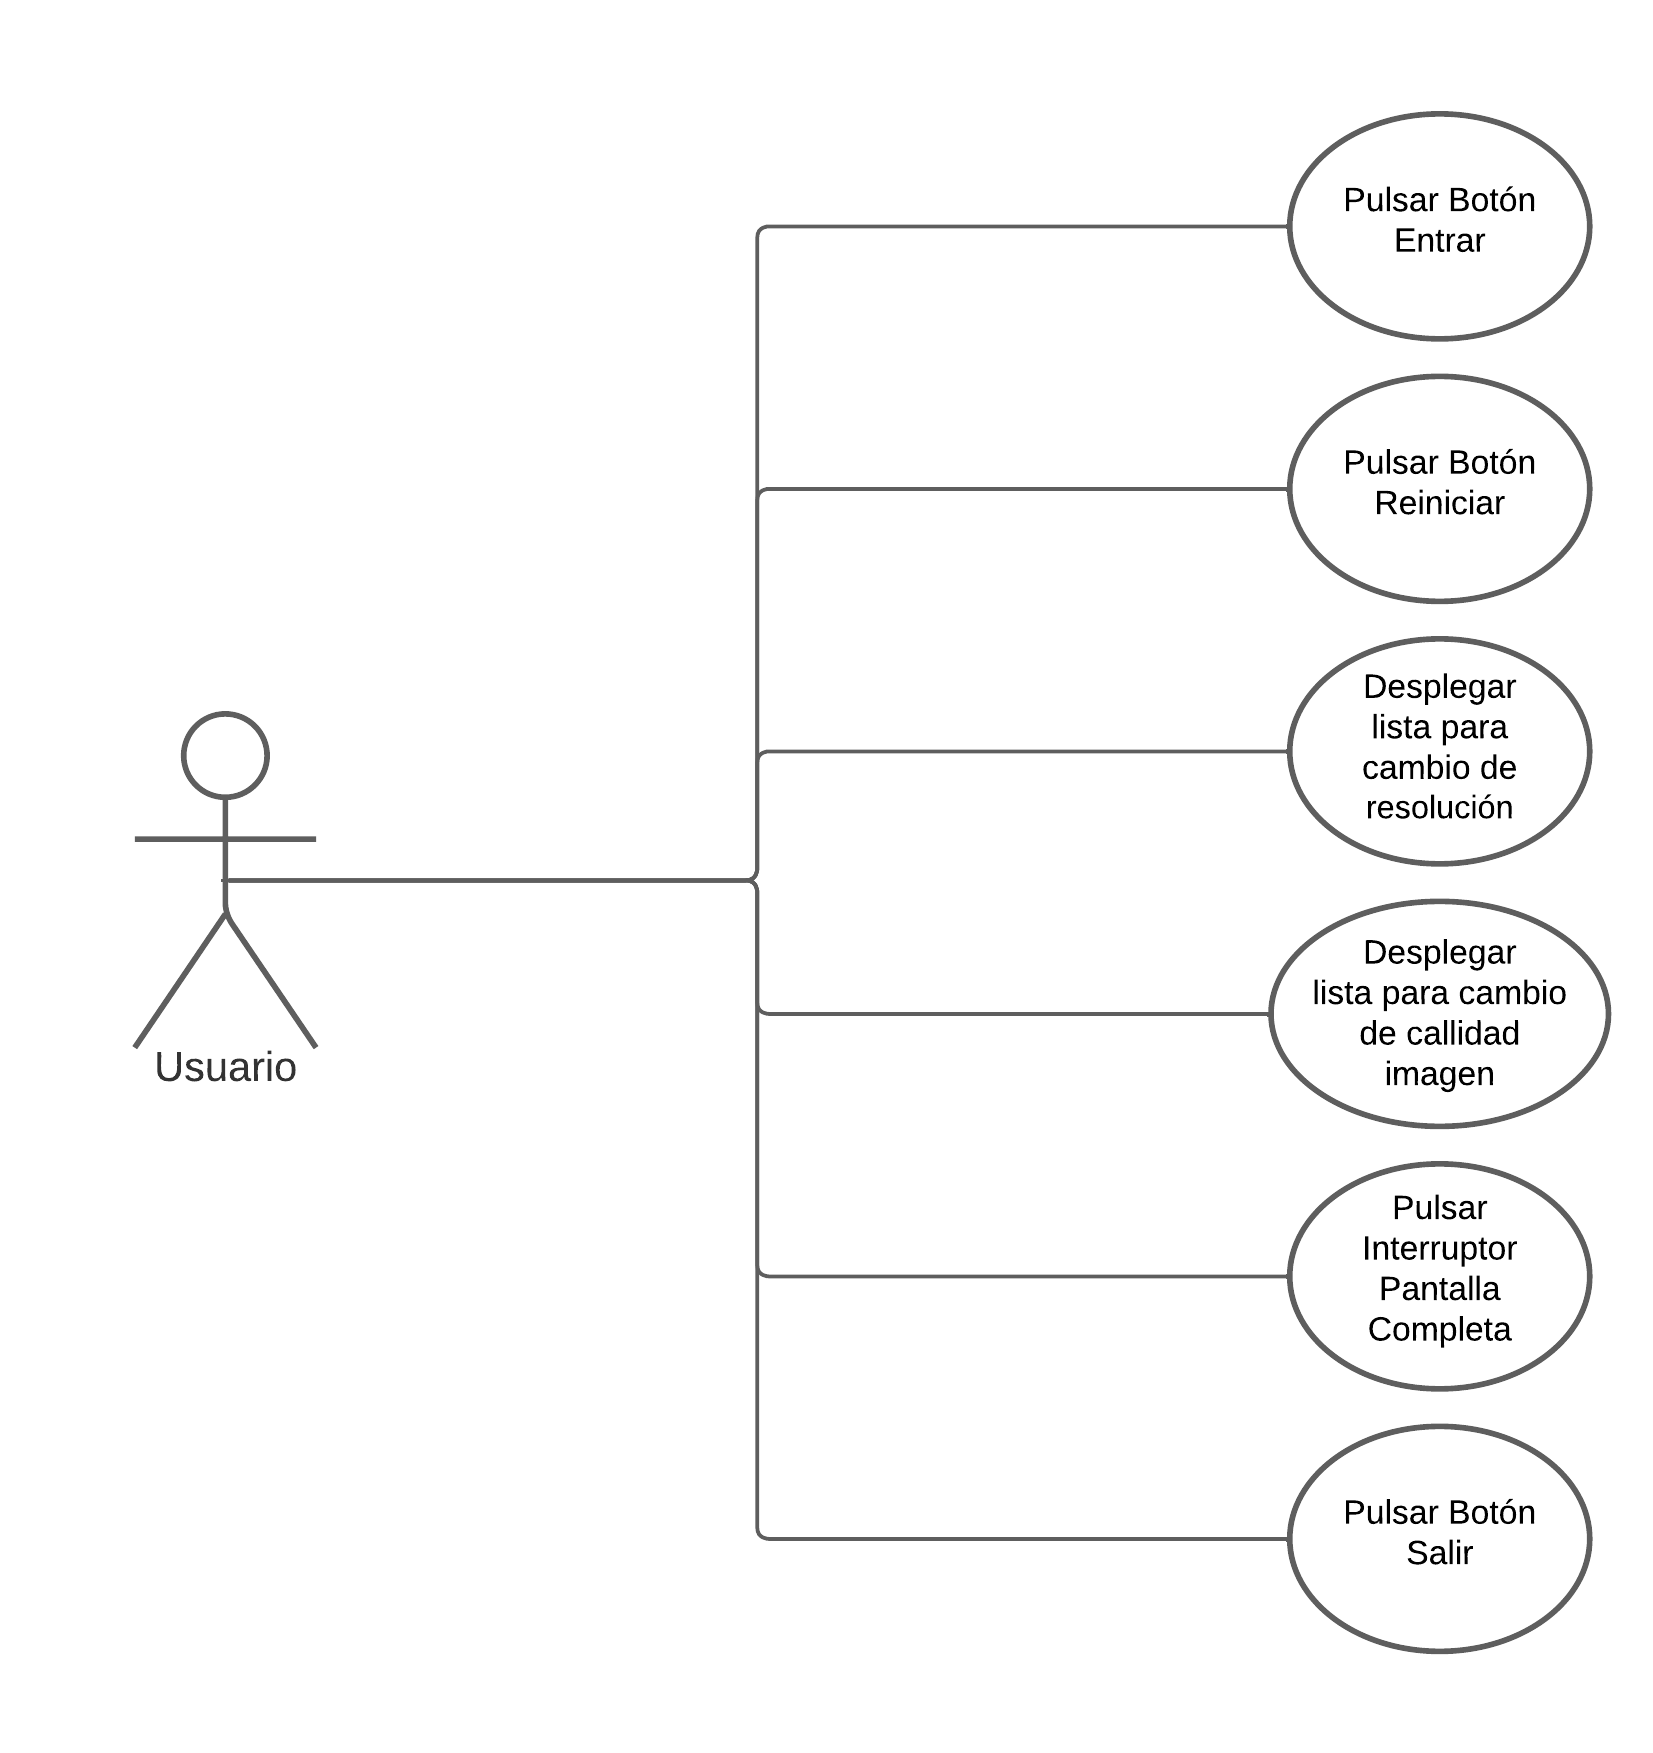
\includegraphics[width=13cm, height=13cm]{figures/cuui.png}
\caption{Diagrama de caso de uso: Usuario}
\label{fig:cuui}
\end{figure}

Como se logra apreciar en la Figura ~\ref{fig:cuui}, se enfoca en la configuración y ajuste de parámetros de la aplicación. Desde reiniciar la simulación hasta cambiar la resolución y calidad de la imagen, estos casos ofrecen opciones para personalizar la configuración de la aplicación según las preferencias del usuario y asi poder abarcar más equipos, por ejemplo, con menos recursos.


\textbf{Caso de uso: Uso de Interfaz dentro de simulación}
\begin{figure}[h]
\centering
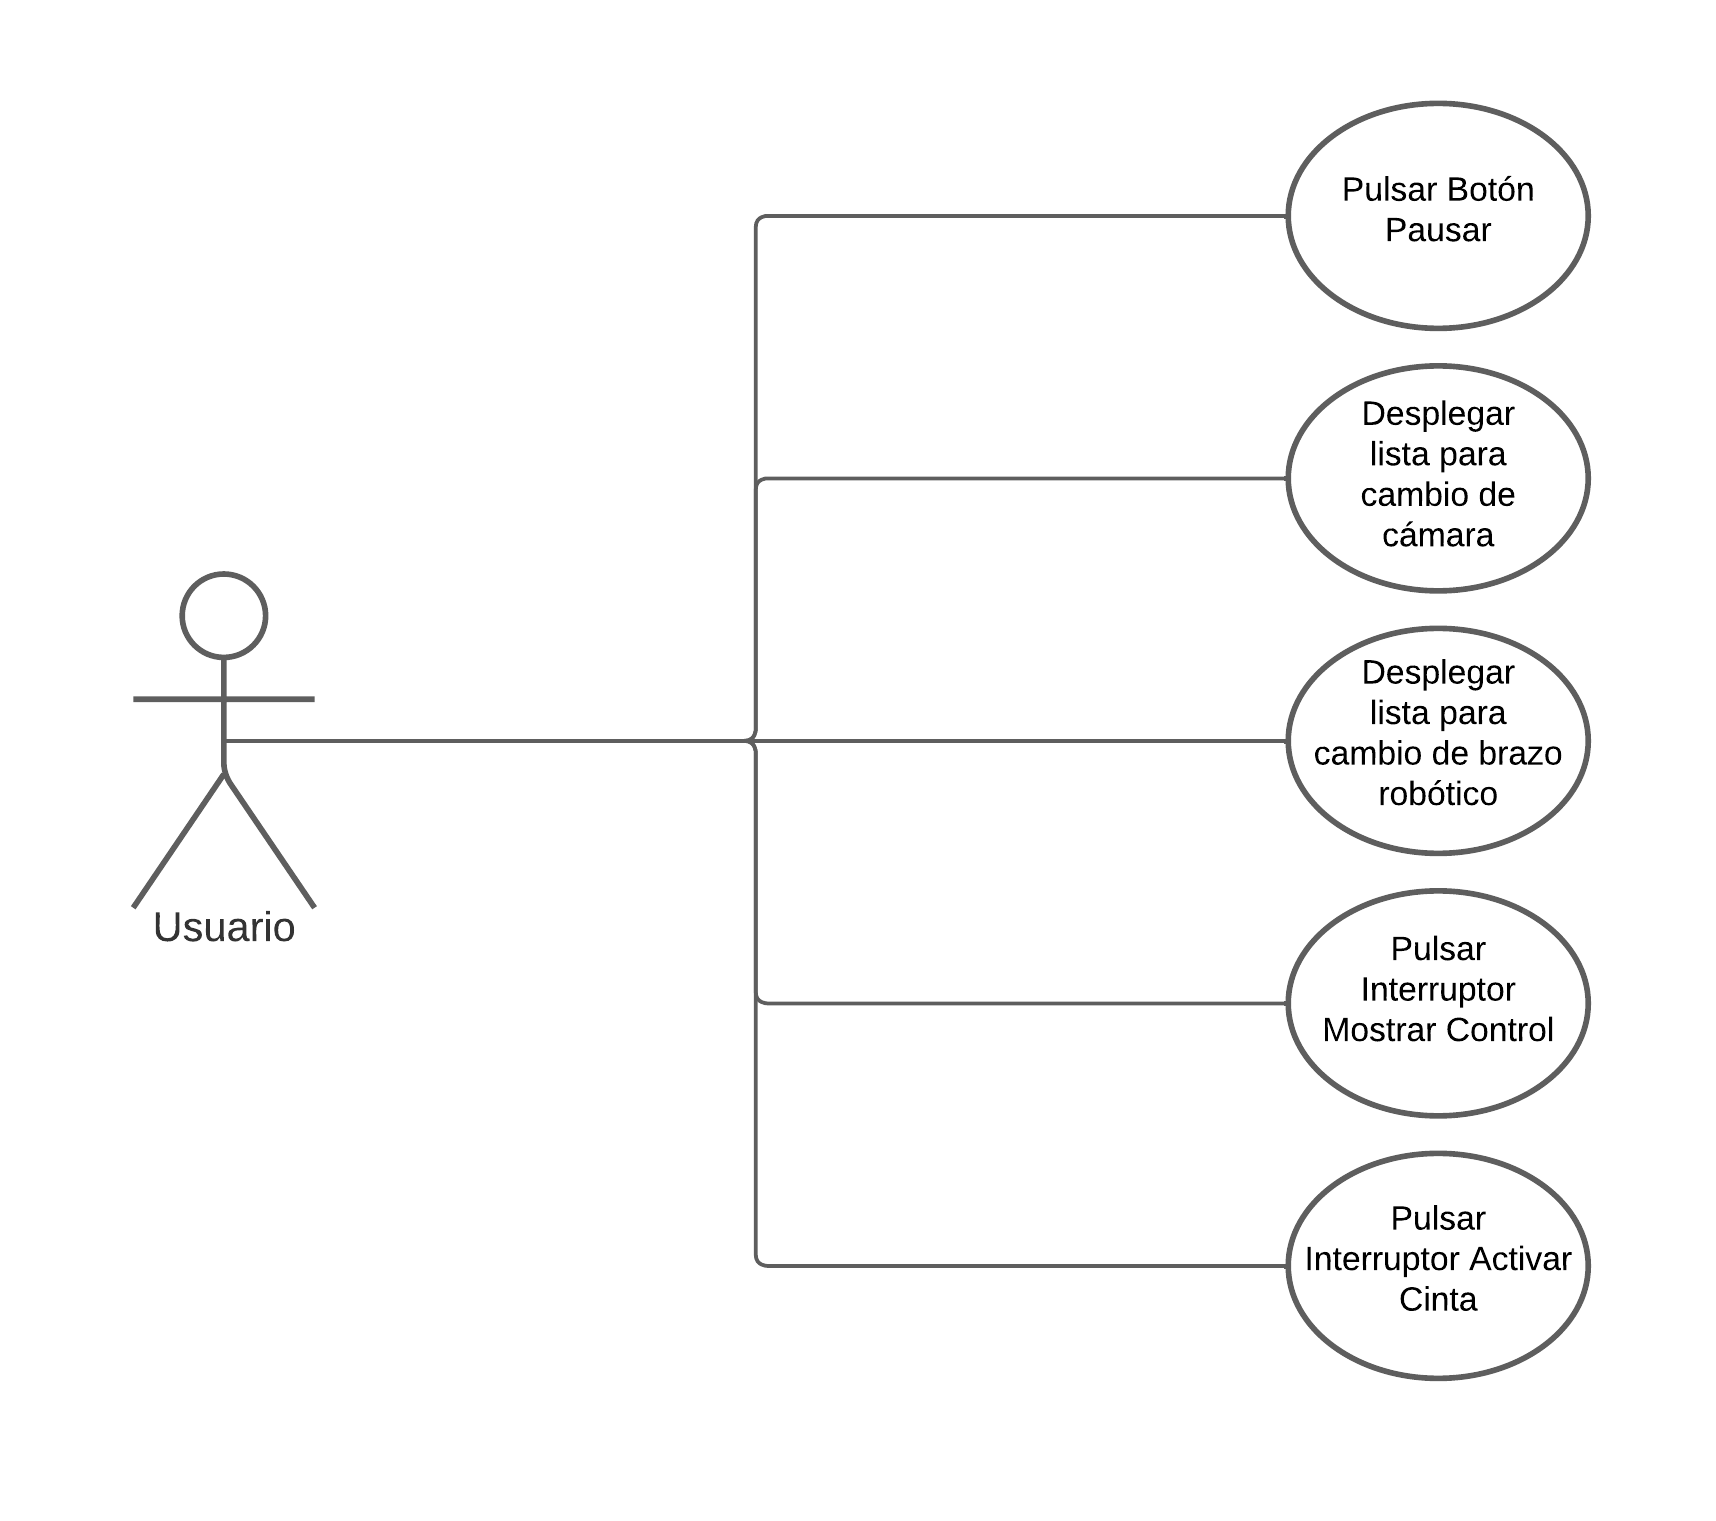
\includegraphics[width=13cm, height=12cm]{figures/cuuisimulacion.png}
\caption{Diagrama de caso de uso: Usuario}
\label{fig:cuuisimulacion}
\end{figure}

Como se logra apreciar en la Figura ~\ref{fig:cuuisimulacion}, esta aborda la navegación y visualización en el sistema. Desde cambiar cámaras hasta activar o desactivar funciones, estos casos permiten a los usuarios personalizar su experiencia de visualización de manera eficiente, cambiar el dispositivo a controlar y cambiar el estado de la cinta transportadora.

\clearpage
\textbf{Caso de uso: Uso de Botonera}
\begin{figure}[h]
\centering
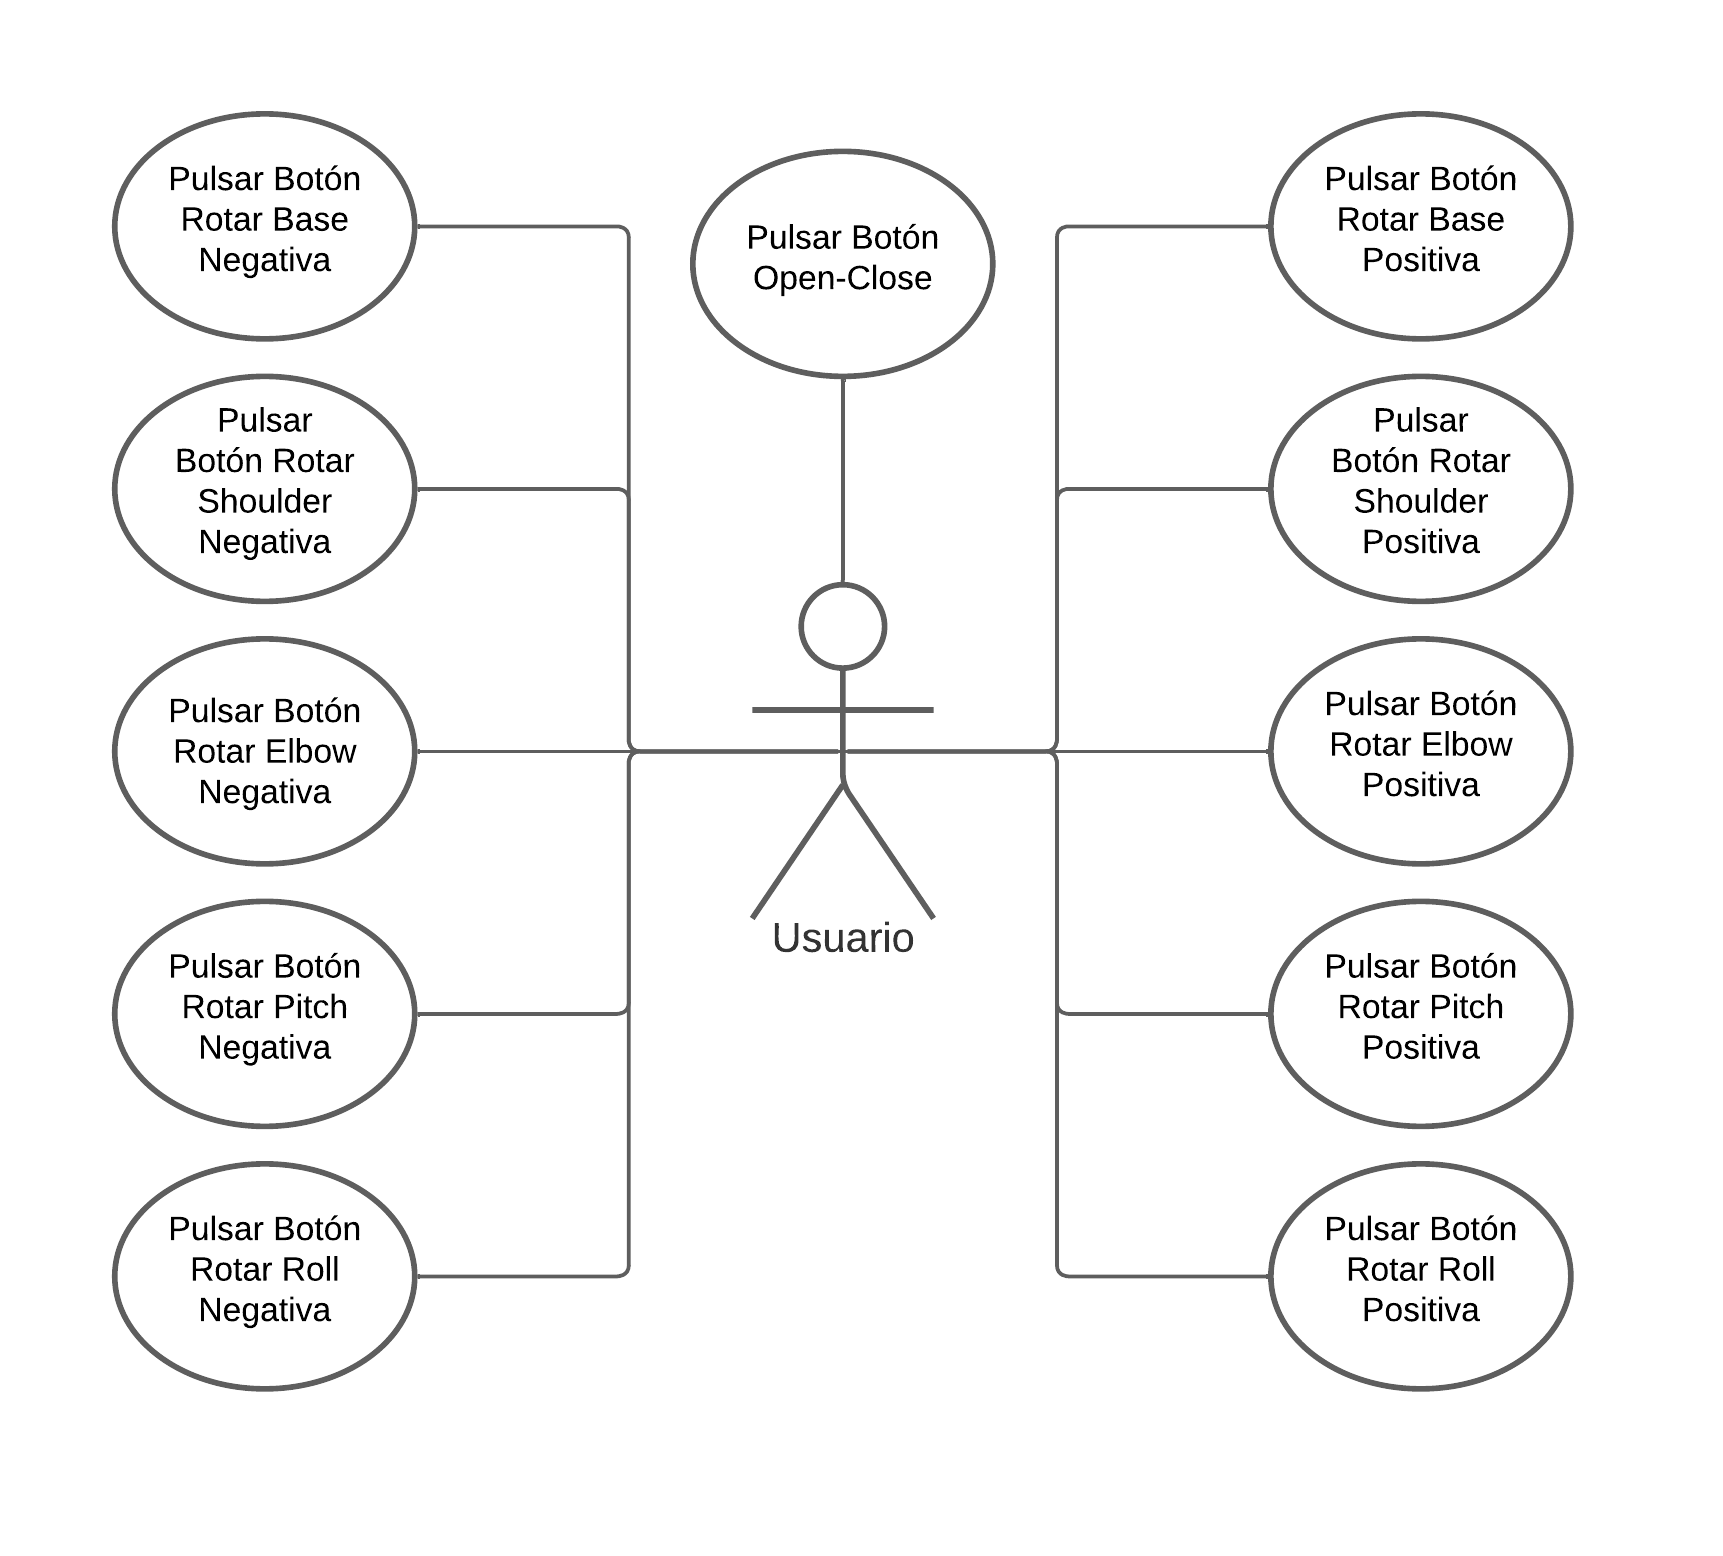
\includegraphics[width=13cm, height=12cm]{figures/cubotonera.png}
\caption{Diagrama de caso de uso: Usuario}
\label{fig:cubotonera}
\end{figure}

Como se logra apreciar en la Figura ~\ref{fig:cubotonera}, se centra en las diversas acciones de movimiento del brazo robot que se encuentran operativas en la botonera. Desde la rotación de articulaciones hasta el control de la pinza, estos casos proporcionan un panorama completo de las capacidades de manipulación del sistema.

\clearpage
\subsection{Especificación de los caso de uso}

\begin{table}[h!]
\begin{center}
\begin{tabular}{| m{0.19\linewidth} | m{0.75\linewidth} |}
\hline
\multicolumn{2}{ |c| }{Caso de Uso: Pulsar Botón Rotar Base Negativa} \\ \hline
ID & CU-01 \\ \hline
Descripción & El actor puede rotar la base del brazo robot en sentido negativo al pulsar el botón correspondiente. \\ \hline
Actores & Usuario \\ \hline
Flujo principal & 

\begin{enumerate}[label=\arabic*.-]
\item El actor visualiza el control de brazo robot.
\item El actor localiza el botón de "Rotar Base Negativa".
\item El actor pulsa el botón de "Rotar Base Negativa".
\end{enumerate}

\\ \hline
\end{tabular}
\caption{Especificación de casos de uso: Pulsar Botón Rotar Base Negativa}
\end{center}
\end{table}

\begin{table}[h!]
\begin{center}
\begin{tabular}{| m{0.19\linewidth} | m{0.75\linewidth} |}
\hline
\multicolumn{2}{ |c| }{Caso de Uso: Pulsar Botón Rotar Base Positiva} \\ \hline
ID & CU-02 \\ \hline
Descripción & El actor puede rotar la base del brazo robot en sentido positivo al pulsar el botón correspondiente. \\ \hline
Actores & Usuario \\ \hline
Flujo principal & 

\begin{enumerate}[label=\arabic*.-]
\item El actor visualiza el control de brazo robot.
\item El actor localiza el botón de "Rotar Base Positiva".
\item El actor pulsa el botón de "Rotar Base Positiva".
\end{enumerate}

\\ \hline
\end{tabular}
\caption{Especificación de casos de uso: Pulsar Botón Rotar Base Positiva}
\end{center}
\end{table}

\begin{table}[h!]
\begin{center}
\begin{tabular}{| m{0.19\linewidth} | m{0.75\linewidth} |}
\hline
\multicolumn{2}{ |c| }{Caso de Uso: Pulsar Botón Pausar} \\ \hline
ID & CU-03 \\ \hline
Descripción & El actor puede pausar las funciones del brazo robot al pulsar el botón correspondiente. \\ \hline
Actores & Usuario \\ \hline
Flujo principal & 

\begin{enumerate}[label=\arabic*.-]
\item El actor visualiza el control de brazo robot.
\item El actor localiza el botón de "Pausar".
\item El actor pulsa el botón de "Pausar".
\end{enumerate}

\\ \hline
\end{tabular}
\caption{Especificación de casos de uso: Pulsar Botón Pausar}
\end{center}
\end{table}


\begin{table}[h!]
\begin{center}
\begin{tabular}{| m{0.19\linewidth} | m{0.75\linewidth} |}
\hline
\multicolumn{2}{ |c| }{Caso de Uso: Desplegar lista para cambio de cámara} \\ \hline
ID & CU-04 \\ \hline
Descripción & El actor puede acceder a una lista para cambiar la cámara del sistema al seleccionar la opción correspondiente. \\ \hline
Actores & Usuario \\ \hline
Flujo principal & 

\begin{enumerate}[label=\arabic*.-]
\item El actor visualiza el control de brazo robot.
\item El actor localiza la opción para "Cambio de Cámara".
\item El actor despliega la lista para cambio de cámara.
\end{enumerate}

\\ \hline
\end{tabular}
\caption{Especificación de casos de uso: Desplegar lista para cambio de cámara}
\end{center}
\end{table}

\begin{table}[h!]
\begin{center}
\begin{tabular}{| m{0.19\linewidth} | m{0.75\linewidth} |}
\hline
\multicolumn{2}{ |c| }{Caso de Uso: Desplegar lista para cambio de brazo robótico} \\ \hline
ID & CU-05 \\ \hline
Descripción & El actor puede acceder a una lista para cambiar el brazo robótico al seleccionar la opción correspondiente. \\ \hline
Actores & Usuario \\ \hline
Flujo principal & 

\begin{enumerate}[label=\arabic*.-]
\item El actor visualiza el control de brazo robot.
\item El actor localiza la opción para "Cambio de Brazo Robótico".
\item El actor despliega la lista para cambio de brazo robótico.
\end{enumerate}

\\ \hline
\end{tabular}
\caption{Especificación de casos de uso: Desplegar lista para cambio de brazo robótico}
\end{center}
\end{table}

\begin{table}[h!]
\begin{center}
\begin{tabular}{| m{0.19\linewidth} | m{0.75\linewidth} |}
\hline
\multicolumn{2}{ |c| }{Caso de Uso: Pulsar Interruptor Mostrar Control} \\ \hline
ID & CU-06 \\ \hline
Descripción & El actor puede mostrar u ocultar el control del brazo robot al pulsar el interruptor correspondiente. \\ \hline
Actores & Usuario \\ \hline
Flujo principal & 

\begin{enumerate}[label=\arabic*.-]
\item El actor visualiza el control de brazo robot.
\item El actor localiza el interruptor para "Mostrar Control".
\item El actor pulsa el interruptor para mostrar u ocultar el control.
\end{enumerate}

\\ \hline
\end{tabular}
\caption{Especificación de casos de uso: Pulsar Interruptor Mostrar Control}
\end{center}
\end{table}

\begin{table}[h!]
\begin{center}
\begin{tabular}{| m{0.19\linewidth} | m{0.75\linewidth} |}
\hline
\multicolumn{2}{ |c| }{Caso de Uso: Pulsar Interruptor Activar Cinta} \\ \hline
ID & CU-07 \\ \hline
Descripción & El actor puede activar o desactivar la cinta del brazo robot al pulsar el interruptor correspondiente. \\ \hline
Actores & Usuario \\ \hline
Flujo principal & 

\begin{enumerate}[label=\arabic*.-]
\item El actor visualiza el control de brazo robot.
\item El actor localiza el interruptor para "Activar Cinta".
\item El actor pulsa el interruptor para activar o desactivar la cinta.
\end{enumerate}

\\ \hline
\end{tabular}
\caption{Especificación de casos de uso: Pulsar Interruptor Activar Cinta}
\end{center}
\end{table}

\begin{table}[h!]
\begin{center}
\begin{tabular}{| m{0.19\linewidth} | m{0.75\linewidth} |}
\hline
\multicolumn{2}{ |c| }{Caso de Uso: Pulsar Botón Reiniciar} \\ \hline
ID & CU-08 \\ \hline
Descripción & El actor puede reiniciar el sistema del brazo robot al pulsar el botón correspondiente. \\ \hline
Actores & Usuario \\ \hline
Flujo principal & 

\begin{enumerate}[label=\arabic*.-]
\item El actor visualiza el control de brazo robot.
\item El actor localiza el botón de "Reiniciar".
\item El actor pulsa el botón de "Reiniciar".
\end{enumerate}

\\ \hline
\end{tabular}
\caption{Especificación de casos de uso: Pulsar Botón Reiniciar}
\end{center}
\end{table}

\begin{table}[h!]
\begin{center}
\begin{tabular}{| m{0.19\linewidth} | m{0.75\linewidth} |}
\hline
\multicolumn{2}{ |c| }{Caso de Uso: Pulsar Botón Entrar} \\ \hline
ID & CU-09 \\ \hline
Descripción & El actor puede ingresar al sistema al pulsar el botón correspondiente. \\ \hline
Actores & Usuario \\ \hline
Flujo principal & 

\begin{enumerate}[label=\arabic*.-]
\item El actor visualiza el control de brazo robot.
\item El actor localiza el botón de "Entrar".
\item El actor pulsa el botón de "Entrar".
\end{enumerate}

\\ \hline
\end{tabular}
\caption{Especificación de casos de uso: Pulsar Botón Entrar}
\end{center}
\end{table}

\begin{table}[h!]
\begin{center}
\begin{tabular}{| m{0.19\linewidth} | m{0.75\linewidth} |}
\hline
\multicolumn{2}{ |c| }{Caso de Uso: Desplegar lista para cambio de resolución} \\ \hline
ID & CU-10 \\ \hline
Descripción & El actor puede acceder a una lista para cambiar la resolución del sistema al seleccionar la opción correspondiente. \\ \hline
Actores & Usuario \\ \hline
Flujo principal & 

\begin{enumerate}[label=\arabic*.-]
\item El actor visualiza el control de brazo robot.
\item El actor localiza la opción para "Cambio de Resolución".
\item El actor despliega la lista para cambio de resolución.
\end{enumerate}

\\ \hline
\end{tabular}
\caption{Especificación de casos de uso: Desplegar lista para cambio de resolución}
\end{center}
\end{table}

\begin{table}[h!]
\begin{center}
\begin{tabular}{| m{0.19\linewidth} | m{0.75\linewidth} |}
\hline
\multicolumn{2}{ |c| }{Caso de Uso: Desplegar lista para cambio de calidad imagen} \\ \hline
ID & CU-11 \\ \hline
Descripción & El actor puede acceder a una lista para cambiar la calidad de la imagen del sistema al seleccionar la opción correspondiente. \\ \hline
Actores & Usuario \\ \hline
Flujo principal & 

\begin{enumerate}[label=\arabic*.-]
\item El actor visualiza el control de brazo robot.
\item El actor localiza la opción para "Cambio de Calidad de Imagen".
\item El actor despliega la lista para cambio de calidad de imagen.
\end{enumerate}

\\ \hline
\end{tabular}
\caption{Especificación de casos de uso: Desplegar lista para cambio de calidad imagen}
\end{center}
\end{table}

\begin{table}[h!]
\begin{center}
\begin{tabular}{| m{0.19\linewidth} | m{0.75\linewidth} |}
\hline
\multicolumn{2}{ |c| }{Caso de Uso: Pulsar Interruptor Pantalla Completa} \\ \hline
ID & CU-12 \\ \hline
Descripción & El actor puede activar o desactivar el modo de pantalla completa al pulsar el interruptor correspondiente. \\ \hline
Actores & Usuario \\ \hline
Flujo principal & 

\begin{enumerate}[label=\arabic*.-]
\item El actor visualiza el control de brazo robot.
\item El actor localiza el interruptor para "Pantalla Completa".
\item El actor pulsa el interruptor para activar o desactivar la pantalla completa.
\end{enumerate}

\\ \hline
\end{tabular}
\caption{Especificación de casos de uso: Pulsar Interruptor Pantalla Completa}
\end{center}
\end{table}

\begin{table}[h!]
\begin{center}
\begin{tabular}{| m{0.19\linewidth} | m{0.75\linewidth} |}
\hline
\multicolumn{2}{ |c| }{Caso de Uso: Pulsar Botón Salir} \\ \hline
ID & CU-13 \\ \hline
Descripción & El actor puede salir del sistema al pulsar el botón correspondiente. \\ \hline
Actores & Usuario \\ \hline
Flujo principal & 

\begin{enumerate}[label=\arabic*.-]
\item El actor visualiza el control de brazo robot.
\item El actor localiza el botón de "Salir".
\item El actor pulsa el botón de "Salir".
\end{enumerate}

\\ \hline
\end{tabular}
\caption{Especificación de casos de uso: Pulsar Botón Salir}
\end{center}
\end{table}

\begin{table}[h!]
\begin{center}
\begin{tabular}{| m{0.19\linewidth} | m{0.75\linewidth} |}
\hline
\multicolumn{2}{ |c| }{Caso de Uso: Pulsar Botón Rotar Shoulder Negativa} \\ \hline
ID & CU-14 \\ \hline
Descripción & El actor puede rotar la articulación "Shoulder" en sentido negativo al pulsar el botón correspondiente. \\ \hline
Actores & Usuario \\ \hline
Flujo principal & 

\begin{enumerate}[label=\arabic*.-]
\item El actor visualiza el control de brazo robot.
\item El actor localiza el botón de "Rotar Shoulder Negativa".
\item El actor pulsa el botón de "Rotar Shoulder Negativa".
\end{enumerate}

\\ \hline
\end{tabular}
\caption{Especificación de casos de uso: Pulsar Botón Rotar Shoulder Negativa}
\end{center}
\end{table}

\begin{table}[h!]
\begin{center}
\begin{tabular}{| m{0.19\linewidth} | m{0.75\linewidth} |}
\hline
\multicolumn{2}{ |c| }{Caso de Uso: Pulsar Botón Rotar Shoulder Positiva} \\ \hline
ID & CU-15 \\ \hline
Descripción & El actor puede rotar la articulación "Shoulder" en sentido positivo al pulsar el botón correspondiente. \\ \hline
Actores & Usuario \\ \hline
Flujo principal & 

\begin{enumerate}[label=\arabic*.-]
\item El actor visualiza el control de brazo robot.
\item El actor localiza el botón de "Rotar Shoulder Positiva".
\item El actor pulsa el botón de "Rotar Shoulder Positiva".
\end{enumerate}

\\ \hline
\end{tabular}
\caption{Especificación de casos de uso: Pulsar Botón Rotar Shoulder Positiva}
\end{center}
\end{table}

\begin{table}[h!]
\begin{center}
\begin{tabular}{| m{0.19\linewidth} | m{0.75\linewidth} |}
\hline
\multicolumn{2}{ |c| }{Caso de Uso: Pulsar Botón Open-Close} \\ \hline
ID & CU-16 \\ \hline
Descripción & El actor puede abrir o cerrar la pinza del brazo robot al pulsar el botón correspondiente. \\ \hline
Actores & Usuario \\ \hline
Flujo principal & 

\begin{enumerate}[label=\arabic*.-]
\item El actor visualiza el control de brazo robot.
\item El actor localiza el botón "Open-Close".
\item El actor pulsa el botón para abrir o cerrar la pinza.
\end{enumerate}

\\ \hline
\end{tabular}
\caption{Especificación de casos de uso: Pulsar Botón Open-Close}
\end{center}
\end{table}

\begin{table}[h!]
\begin{center}
\begin{tabular}{| m{0.19\linewidth} | m{0.75\linewidth} |}
\hline
\multicolumn{2}{ |c| }{Caso de Uso: Pulsar Botón Rotar Elbow Negativa} \\ \hline
ID & CU-17 \\ \hline
Descripción & El actor puede rotar la articulación "Elbow" en sentido negativo al pulsar el botón correspondiente. \\ \hline
Actores & Usuario \\ \hline
Flujo principal & 

\begin{enumerate}[label=\arabic*.-]
\item El actor visualiza el control de brazo robot.
\item El actor localiza el botón de "Rotar Elbow Negativa".
\item El actor pulsa el botón de "Rotar Elbow Negativa".
\end{enumerate}

\\ \hline
\end{tabular}
\caption{Especificación de casos de uso: Pulsar Botón Rotar Elbow Negativa}
\end{center}
\end{table}

\begin{table}[h!]
\begin{center}
\begin{tabular}{| m{0.19\linewidth} | m{0.75\linewidth} |}
\hline
\multicolumn{2}{ |c| }{Caso de Uso: Pulsar Botón Rotar Elbow Positiva} \\ \hline
ID & CU-18 \\ \hline
Descripción & El actor puede rotar la articulación "Elbow" en sentido positivo al pulsar el botón correspondiente. \\ \hline
Actores & Usuario \\ \hline
Flujo principal & 

\begin{enumerate}[label=\arabic*.-]
\item El actor visualiza el control de brazo robot.
\item El actor localiza el botón de "Rotar Elbow Positiva".
\item El actor pulsa el botón de "Rotar Elbow Positiva".
\end{enumerate}

\\ \hline
\end{tabular}
\caption{Especificación de casos de uso: Pulsar Botón Rotar Elbow Positiva}
\end{center}
\end{table}

\begin{table}[h!]
\begin{center}
\begin{tabular}{| m{0.19\linewidth} | m{0.75\linewidth} |}
\hline
\multicolumn{2}{ |c| }{Caso de Uso: Pulsar Botón Rotar Pitch Negativa} \\ \hline
ID & CU-19 \\ \hline
Descripción & El actor puede rotar la articulación "Pitch" en sentido negativo al pulsar el botón correspondiente. \\ \hline
Actores & Usuario \\ \hline
Flujo principal & 

\begin{enumerate}[label=\arabic*.-]
\item El actor visualiza el control de brazo robot.
\item El actor localiza el botón de "Rotar Pitch Negativa".
\item El actor pulsa el botón de "Rotar Pitch Negativa".
\end{enumerate}

\\ \hline
\end{tabular}
\caption{Especificación de casos de uso: Pulsar Botón Rotar Pitch Negativa}
\end{center}
\end{table}

\begin{table}[h!]
\begin{center}
\begin{tabular}{| m{0.19\linewidth} | m{0.75\linewidth} |}
\hline
\multicolumn{2}{ |c| }{Caso de Uso: Pulsar Botón Rotar Pitch Positiva} \\ \hline
ID & CU-20 \\ \hline
Descripción & El actor puede rotar la articulación "Pitch" en sentido positivo al pulsar el botón correspondiente. \\ \hline
Actores & Usuario \\ \hline
Flujo principal & 

\begin{enumerate}[label=\arabic*.-]
\item El actor visualiza el control de brazo robot.
\item El actor localiza el botón de "Rotar Pitch Positiva".
\item El actor pulsa el botón de "Rotar Pitch Positiva".
\end{enumerate}

\\ \hline
\end{tabular}
\caption{Especificación de casos de uso: Pulsar Botón Rotar Pitch Positiva}
\end{center}
\end{table}

\begin{table}[h!]
\begin{center}
\begin{tabular}{| m{0.19\linewidth} | m{0.75\linewidth} |}
\hline
\multicolumn{2}{ |c| }{Caso de Uso: Pulsar Botón Rotar Roll Negativa} \\ \hline
ID & CU-21 \\ \hline
Descripción & El actor puede rotar la articulación "Roll" en sentido negativo al pulsar el botón correspondiente. \\ \hline
Actores & Usuario \\ \hline
Flujo principal & 

\begin{enumerate}[label=\arabic*.-]
\item El actor visualiza el control de brazo robot.
\item El actor localiza el botón de "Rotar Roll Negativa".
\item El actor pulsa el botón de "Rotar Roll Negativa".
\end{enumerate}

\\ \hline
\end{tabular}
\caption{Especificación de casos de uso: Pulsar Botón Rotar Roll Negativa}
\end{center}
\end{table}

\begin{table}[h!]
\begin{center}
\begin{tabular}{| m{0.19\linewidth} | m{0.75\linewidth} |}
\hline
\multicolumn{2}{ |c| }{Caso de Uso: Pulsar Botón Rotar Roll Positiva} \\ \hline
ID & CU-22 \\ \hline
Descripción & El actor puede rotar la articulación "Roll" en sentido positivo al pulsar el botón correspondiente. \\ \hline
Actores & Usuario \\ \hline
Flujo principal & 

\begin{enumerate}[label=\arabic*.-]
\item El actor visualiza el control de brazo robot.
\item El actor localiza el botón de "Rotar Roll Positiva".
\item El actor pulsa el botón de "Rotar Roll Positiva".
\end{enumerate}

\\ \hline
\end{tabular}
\caption{Especificación de casos de uso: Pulsar Botón Rotar Roll Positiva}
\end{center}
\end{table}

\chapter{Diseño} \input{capitulos/08diseño}
\chapter{Código} En este capitulo, se presenta explicaciones sobre el código fuente de la aplicación desarrollada.
\section{Lógica Cinta Transportadora}
\lstset{language=[Sharp]C, breaklines=true, basicstyle=\footnotesize}
\begin{lstlisting}[frame=single]
using System;
using System.Collections;
using System.Collections.Generic;
using UnityEngine;

public class Belt : MonoBehaviour
{
    public float speed =5f;
    Rigidbody rBody;
    public Vector3 direccion;

    void Start()
    {
        rBody = GetComponent<Rigidbody>();
    }

    void FixedUpdate()
    {
        Vector3 pos = rBody.position;
        rBody.position += direccion * speed * Time.fixedDeltaTime;
        rBody.MovePosition(pos);
    }
}
\end{lstlisting}
Este código proporciona la lógica simple de movimiento de objetos en la cinta transportadora, sin embargo este no llega a replicar su funcionamiento real debido a limitaciones que se explica en los detalles siguientes:

\begin{lstlisting}[frame=single]
using System;
using System.Collections;
using System.Collections.Generic;
using UnityEngine;
\end{lstlisting}
Estas líneas son declaraciones de uso de espacio de nombres (namespace) que indican qué bibliotecas se están utilizando en el código. Están importando las bibliotecas necesarias para trabajar con Unity y otros espacios de nombres estándar de C\#.

\begin{lstlisting}[frame=single]
public class Belt : MonoBehaviour
{
    ...
}
\end{lstlisting}
Aquí comienza la definición de la clase Belt, que hereda de la clase MonoBehaviour. Esto significa que este script puede ser adjuntado a objetos en Unity y ejecutado como parte del comportamiento de esos objetos.

\begin{lstlisting}[frame=single]
    public float speed =5f;
    Rigidbody rBody;
    public Vector3 direccion;
\end{lstlisting}
En esta parte se declaran las variables, se parte con una variable pública llamada speed (velocidad) que tiene un valor predeterminado de 5. Esta variable representa la velocidad a la que se moverá la cinta transportadora.
Después se declara una variable llamada rBody de tipo Rigidbody. Esta variable se utilizará para almacenar una referencia al componente Rigidbody adjunto al objeto al que se adjunte este script. Un Rigidbody es un componente utilizado en el desarrollo de videojuegos y simulaciones físicas para representar objetos que tienen propiedades físicas, como masa, velocidad, y fuerzas que actúan sobre ellos.
Por ultimo se declara una variable pública llamada direccion (dirección) de tipo Vector3. Vector3 es una estructura de datos utilizada para representar vectores tridimensionales en un espacio tridimensional. Esta variable se utiliza para definir la dirección en la que se moverá la cinta transportadora. La dirección se establece desde el Inspector de Unity cuando adjuntes este script a un objeto en el juego.

\begin{lstlisting}[frame=single]
    void Start()
    {
        rBody = GetComponent<Rigidbody>();
    }
\end{lstlisting}
El método Start() es uno de los métodos especiales en Unity que se llama automáticamente cuando se inicia un objeto al que se adjunta un script, en este caso se obtiene una referencia al componente Rigidbody del objeto al que se adjunta este script. Esto se hace utilizando la función GetComponent<Rigidbody>(), y la referencia se almacena en la variable rBody.
\clearpage
\begin{lstlisting}[frame=single]
    void FixedUpdate()
    {
        ...
    }
\end{lstlisting}
FixedUpdate es un método especial que se encuentra en Unity y es utilizado para realizar cálculos y actualizaciones relacionadas con la física en un juego. A diferencia de Update, que se llama una vez por cada fotograma (frame) renderizado, FixedUpdate se llama en intervalos de tiempo fijos y regulares, lo que lo hace especialmente adecuado para manejar la simulación de física y movimiento en un juego.

\begin{lstlisting}[frame=single]
        Vector3 pos = rBody.position;
\end{lstlisting}
Aquí se crea una variable local llamada pos que almacena la posición actual del objeto asociado al Rigidbody.

\begin{lstlisting}[frame=single]
        rBody.position += direccion * speed * Time.fixedDeltaTime;
\end{lstlisting}
Esta línea actualiza la posición del objeto con el componente Rigidbody (rBody) al agregarle un desplazamiento basado en la dirección (direccion), la velocidad (speed), y el tiempo transcurrido (Time.fixedDeltaTime). Esto aun no simula el movimiento de la cinta transportadora y se explica con las siguientes figuras. 
\begin{figure}[h]
\centering
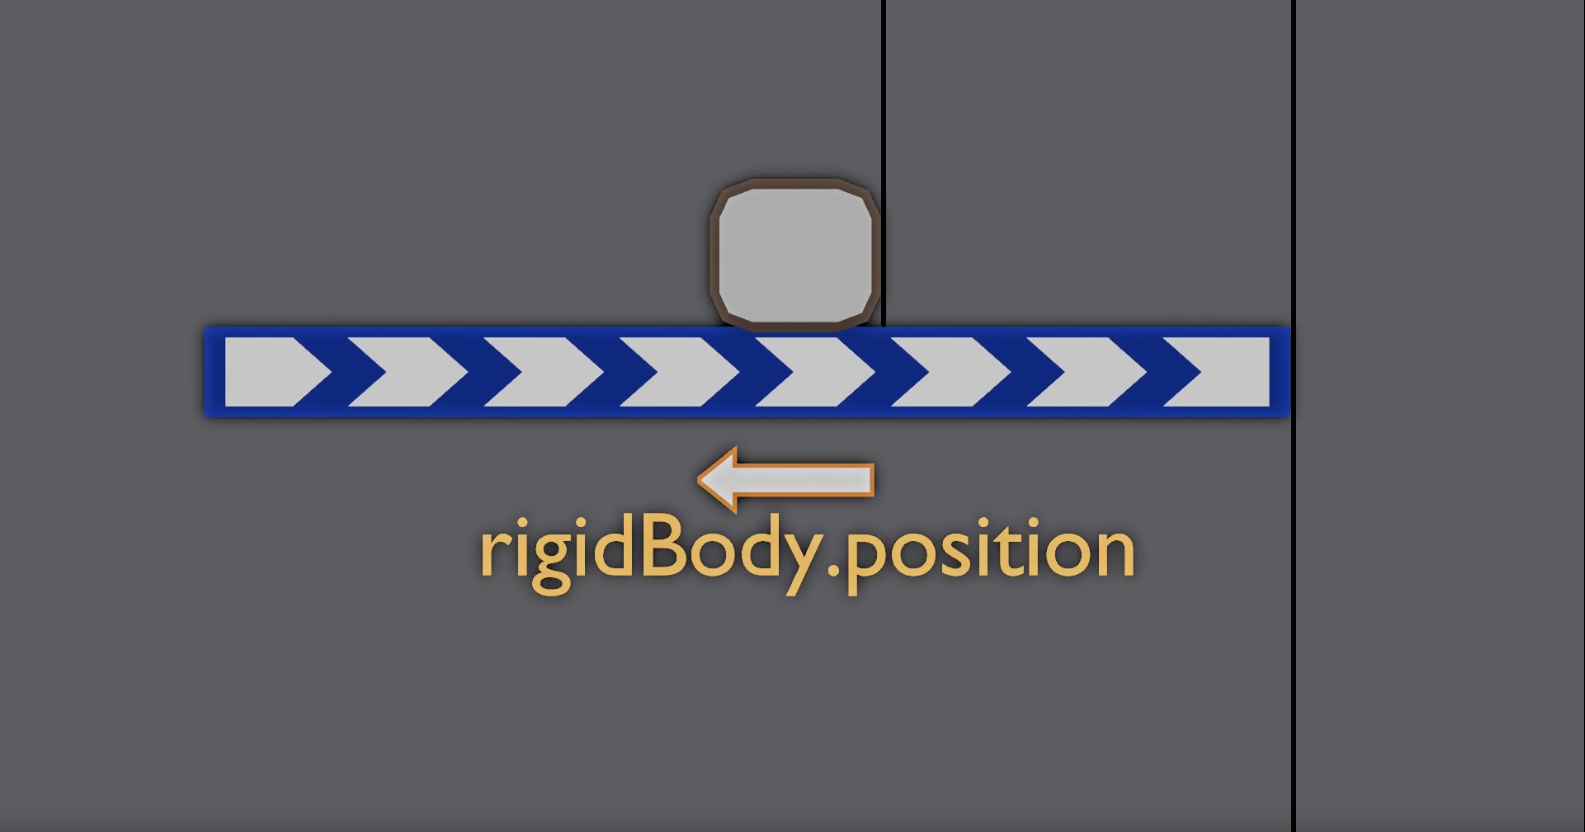
\includegraphics[width=10cm, height=6cm]{figures/rbodyposition1.png}
\caption{rigidBody Position 1}
\label{fig:rbodyposition1}
\end{figure}


En la Figura ~\ref{fig:rbodyposition1} se presenta el movimiento de la cinta, este movimiento solo aplica para la cinta, a diferencia del método MovePosition que se presenta más adelante.
\clearpage

\begin{figure}[h]
\centering
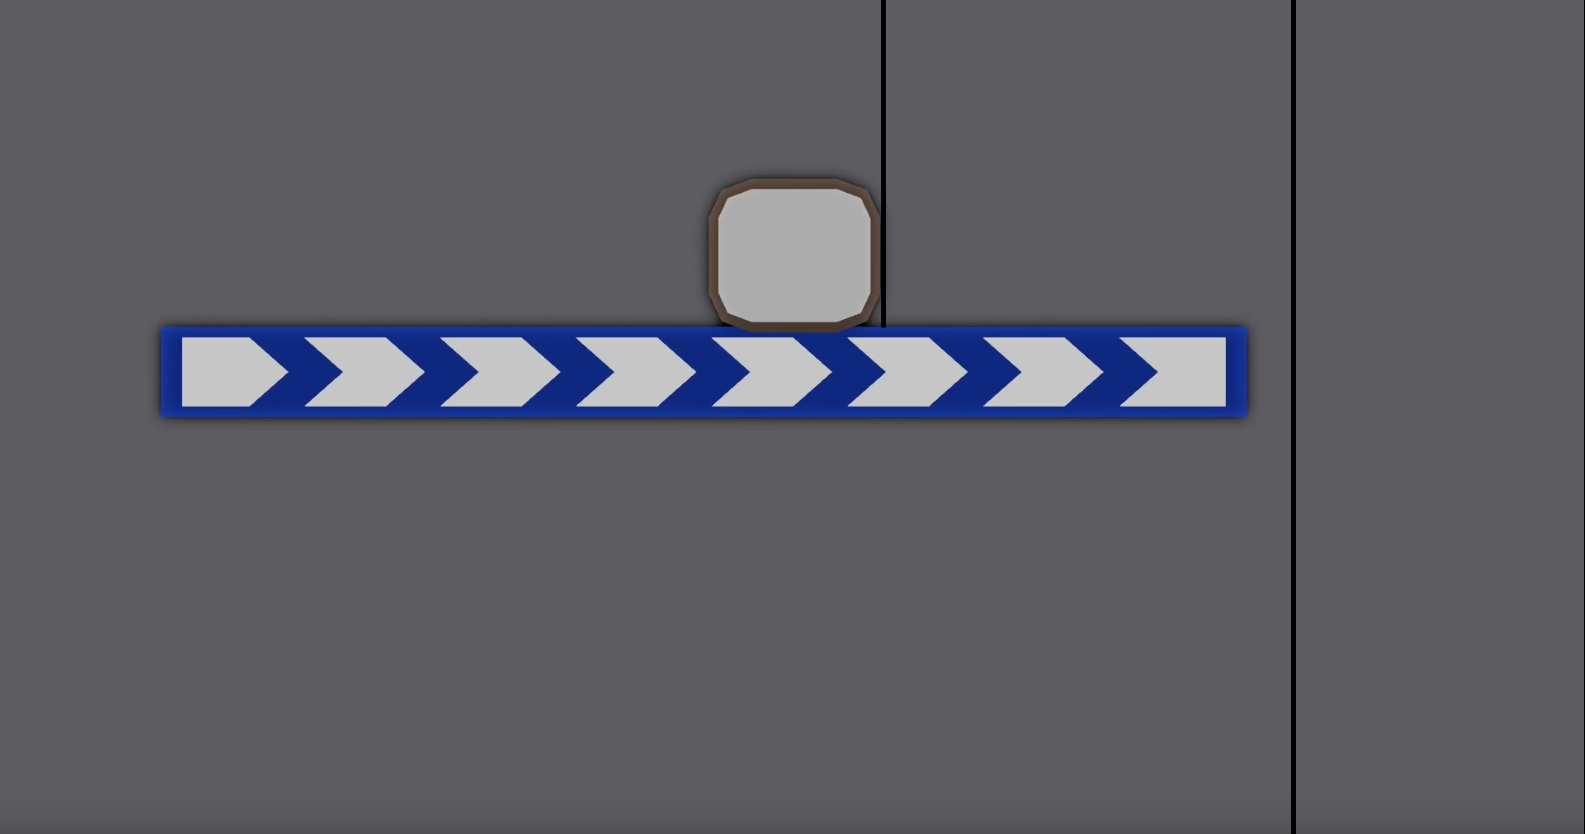
\includegraphics[width=10cm, height=6cm]{figures/rbodyposition2.png}
\caption{rigidBody Position 2}
\label{fig:rbodyposition2}
\end{figure}

En la Figura ~\ref{fig:rbodyposition2} se muestra donde finaliza el movimiento, como se aprecia este solo mueve la cinta y el objeto sobre esta no posee movimiento

\begin{lstlisting}[frame=single]
        rBody.MovePosition(pos);
\end{lstlisting}
En este método, se devuelve la cinta a su posición original, la diferencia que con el método de movimiento anterior es que si se mueve el objeto, tal como se presenta en las siguientes figuras.
\begin{figure}[h]
\centering
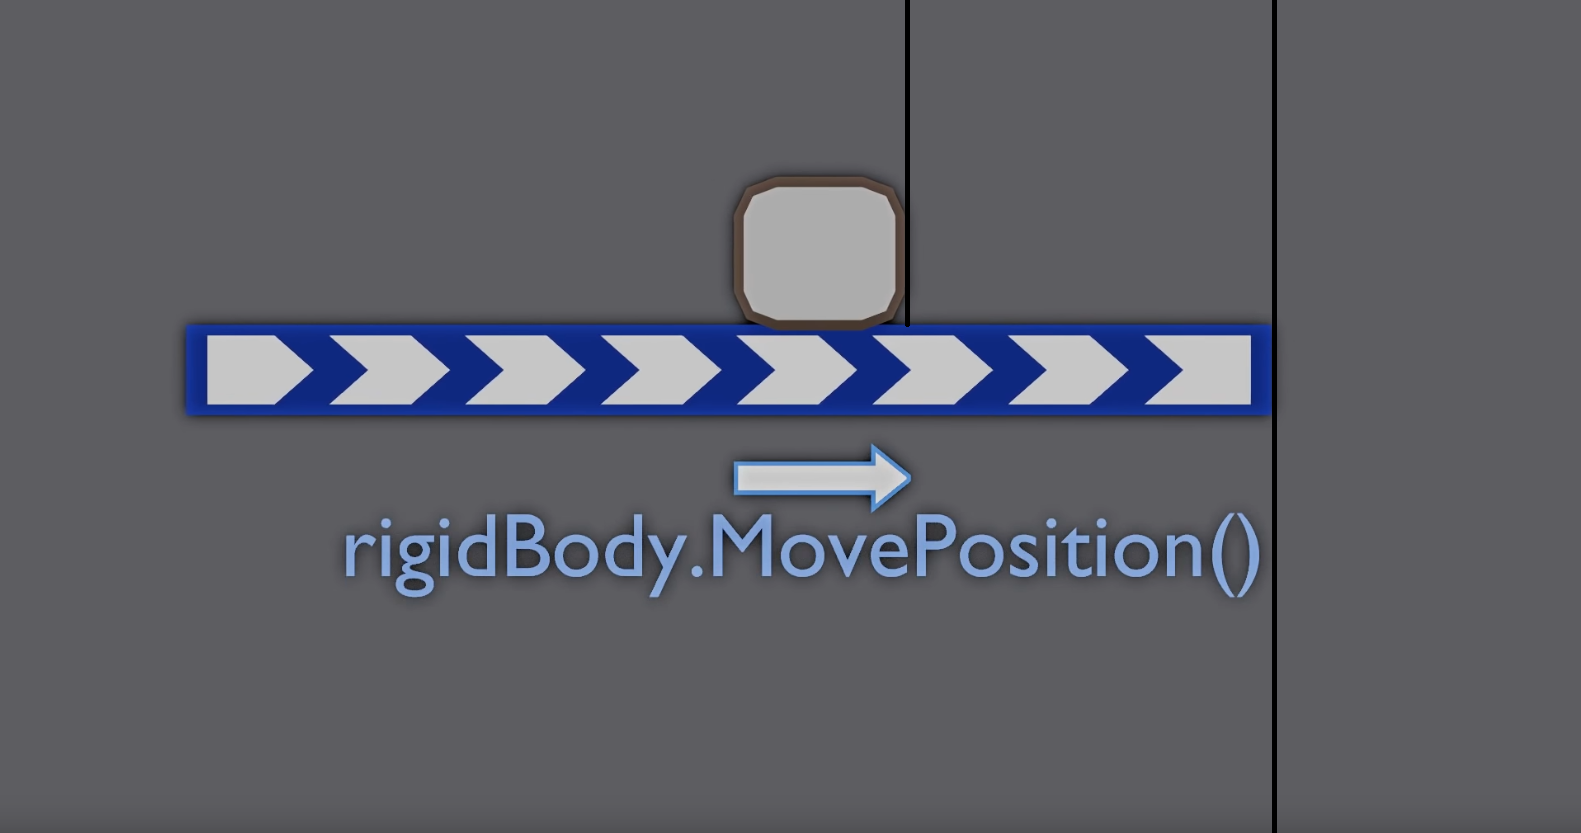
\includegraphics[width=10cm, height=6cm]{figures/rbodymove1.png}
\caption{rigidBody MovePosition 1}
\label{fig:rbodymove1}
\end{figure}

En la Figura ~\ref{fig:rbodymove1} se presenta el movimiento de la cinta, este movimiento aplica tanto para la cinta como para el objeto.

\clearpage

\begin{figure}[h]
\centering
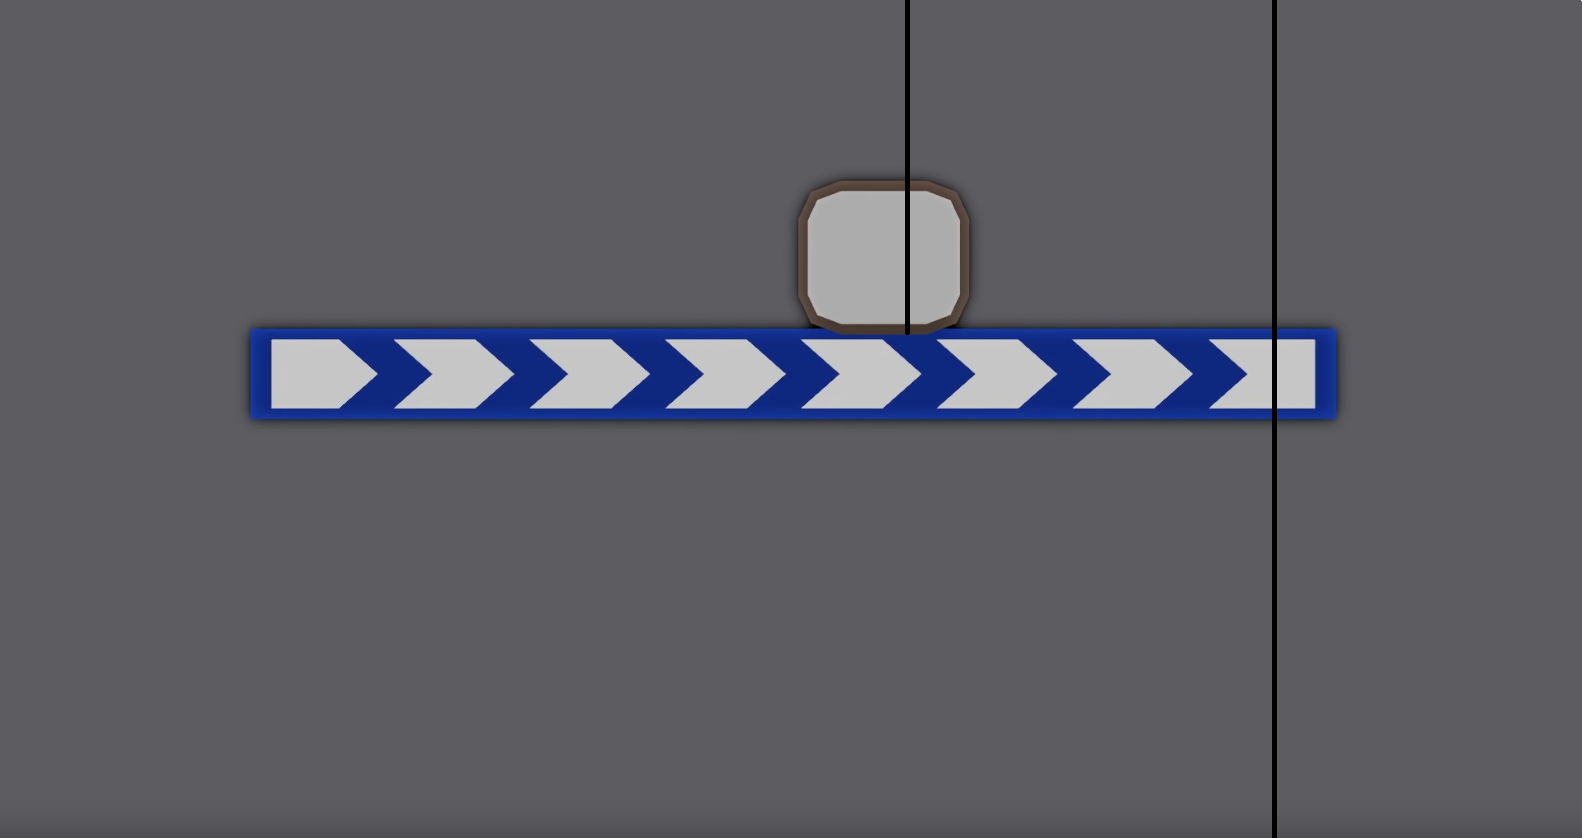
\includegraphics[width=10cm, height=6cm]{figures/rbodymove2.png}
\caption{rigidBody MovePosition 2}
\label{fig:rbodymove2}
\end{figure}

En la Figura ~\ref{fig:rbodymove2} se muestra donde finaliza el movimiento, como se aprecia este mueve tanto la cinta y como el objeto.

Con esta sucesión de movimientos, la cinta al "ir para atrás" sin mover el objeto, y después "volver a su posición" moviendo el objeto, repitiéndolo una y otra vez se logra el efecto de una cinta transportadora. El problema es que el objeto solo se mueve y en las esquinas no rota como en el laboratorio.
\clearpage
\section{Lógica Brazos Robóticos}
Para esta lógica, se explicara los detalles mas importantes debido a que el código es demasiado extenso.
\begin{lstlisting}[frame=single]
   //Base
    public float velocidadRotacionBase = 50.0f; // Velocidad de rotacion
    public KeyCode teclaRotacionPositivaBase = KeyCode.Q; // Tecla para la rotacion en direccion positiva
    public KeyCode teclaRotacionNegativaBase = KeyCode.A; // Tecla para la rotacion en direccion negativa
    public Transform Base; // Transform del objeto que se va a rotar
    private float LimitePositivoBase = 155.0f; // Angulo limite del objeto
    private float LimiteNegativoBase = -155.0f; // Angulo limite del objeto
    private float sumaRotacionBase = 0.0f; // Suma de la rotacion del objeto para su uso en limites

    //Shoulder
    public float velocidadRotacionShoulder = 50.0f; // Velocidad de rotacion
    public KeyCode teclaRotacionPositivaShoulder = KeyCode.W; // Tecla para la rotacion en direccion positiva
    public KeyCode teclaRotacionNegativaShoulder = KeyCode.S; // Tecla para la rotacion en direccion negativa
    public Transform Shoulder; // Transform del objeto a rotar
    public Transform puntoFijoShoulder; // Transform del punto fijo alrededor del cual se realizara la rotacion
    private float LimitePositivoShoulder = 10.0f; // Angulo limite del objeto
    private float LimiteNegativoShoulder = -130.0f; // Angulo limite del objeto
    private float sumaRotacionShoulder = 0.0f; // Suma de la rotacion del objeto para su uso en limites
\end{lstlisting}
Para explicar las declaraciones de las partes de los brazos, se toma en cuenta dos partes distintas pero aplica para cualquier otra parte similar, la base es un objeto que tiene rotación sobre su propio eje, es decir no necesita otro punto para rotar o rota sobre su propio centro, a diferencia del Shoulder o un brazo cualquiera, para rotar este tiene un punto fijo en uno de sus extremos y no en el centro.
Se empieza con declarar la velocidad de la rotación del objeto en una variable float. Después se declaran variables tipo KeyCode que sirven para almacenar la información de una tecla en el teclado en particular, esto se realiza para realizar pruebas de movimiento.
Al declarar una variable de tipo Transform, en Unity, un "Transform" se refiere a un componente fundamental que se encuentra en la mayoría de los objetos en un escenario 3D o 2D. El componente Transform está asociado con la posición, rotación y escala de un objeto en el espacio de juego. Básicamente, controla la ubicación y la orientación de un objeto en el mundo virtual creado en Unity. Con esta variable se puede guardar toda la información previamente descrita, con la finalidad de realizar movimientos. En casos de rotación sobre el mismo objeto como la Base, solo se pide una variable, para objetos con centro en su extremo se piden dos variables, mas adelante se detallara como funciona el movimiento y el motivo de pedir uno o dos variables.
Y por ultimo se tienen los limites, consisten en dos variables que marcan el limite de operación de cada parte, para este caso se utilizan los limites establecidos mecánicamente por la misma unidad descrita en su manual. Y también la suma de rotación, la cual almacenara como tal el movimiento realizado, esto para ser utilizado en la comprobación de limites

\begin{lstlisting}[frame=single]
    private string nombreObjeto = "";
\end{lstlisting}
En esta linea se declara una variable para identificar la parte que se moverá con la botonera.

\begin{lstlisting}[frame=single]
    private bool positivoboton = false;
    private bool negativoboton = false;
\end{lstlisting}
Con estas variables sirven para saber si el botón presionado es positivo o negativo

\begin{lstlisting}[frame=single]
    private bool isControlPressed = false;
    private bool isAltPressed = false;
\end{lstlisting}
Para estas lineas se utilizo para realizar pruebas para guardar posiciones y realizar el movimiento a esa posición, estas servían para saber si Control fue presionado o el Alt fue presionado

\begin{lstlisting}[frame=single]
    private bool EmpezarGuardar = false;
    private bool TerminarGuardar = false;
    private bool EmpezarMover = false;
    private bool TerminarMover = false;
\end{lstlisting}
Acá los booleanos son para lo descrito anteriormente, sirven para marcar los inicios y finales de guardar posiciones y mover a las posiciones

\begin{lstlisting}[frame=single]
    private int NumeroUsar = -1;
\end{lstlisting}
Este numero es el numero usado en la botonera, en el cual se guardara la información.

\begin{lstlisting}[frame=single]
    private Dictionary<int, float> GuardarBase = new Dictionary<int, float>();
    private Dictionary<int, float> GuardarShoulder = new Dictionary<int, float>();
    private Dictionary<int, float> GuardarElbow = new Dictionary<int, float>();
    private Dictionary<int, float> GuardarWrist = new Dictionary<int, float>();
    private Dictionary<int, float> GuardarEndEffector = new Dictionary<int, float>();
\end{lstlisting}
Estas variables son diccionarios, los cuales con una variable devuelve una segunda variable, con esto poder guardar por ejemplo, la posición dependiendo del numero requerido, función que ocupa la botonera. Esta declarada para que con un numero entero devuelva un flotante.

\clearpage
\begin{lstlisting}[frame=single]
    private void Start()
    {
        GuardarBase.Add(0, 0f);
        GuardarShoulder.Add(0,0f);
        GuardarElbow.Add(0,0f);
        GuardarWrist.Add(0,0f);
        GuardarEndEffector.Add(0,0f);
    }
\end{lstlisting}
Al ejecutar el programa, en su inicio ejecutara esta secuencia de funciones, las cuales son para agregar la posición cero a los diccionarios.

\begin{lstlisting}[frame=single]
    private void Update()
    {
        Movimiento(Base, teclaRotacionPositivaBase, teclaRotacionNegativaBase, velocidadRotacionBase, LimitePositivoBase, LimiteNegativoBase, Base, Base.up, ref sumaRotacionBase);
        Movimiento(Shoulder, teclaRotacionPositivaShoulder, teclaRotacionNegativaShoulder, velocidadRotacionShoulder, LimitePositivoShoulder, LimiteNegativoShoulder, puntoFijoShoulder, puntoFijoShoulder.forward, ref sumaRotacionShoulder);
        Movimiento(Elbow, teclaRotacionPositivaElbow, teclaRotacionNegativaElbow, velocidadRotacionElbow, LimitePositivoElbow, LimiteNegativoElbow, puntoFijoElbow, puntoFijoElbow.forward, ref sumaRotacionElbow);
        Movimiento(Wrist, teclaRotacionPositivaWrist, teclaRotacionNegativaWrist, velocidadRotacionWrist, LimitePositivoWrist, LimiteNegativoWrist, puntoFijoWrist, Wrist.forward, ref sumaRotacionWrist);
        Movimiento(EndEffector, teclaRotacionPositivaEndEffector, teclaRotacionNegativaEndEffector, velocidadRotacionEndEffector, LimitePositivoEndEffector, LimiteNegativoEndEffector, puntoFijoEndEffector, EndEffector.right, ref sumaRotacionEndEffector);
        MovimientoBoton(nombreObjeto);
        Guardar();
        Usar();
        GuardarBoton();
        UsarBoton();
        MoverEje();
        MoverEjeBoton();
    }
\end{lstlisting}
El update se encarga de que el programa este esperando una interacción por parte del usuario para realizar una función, las cuales se explicaran a continuación.
\clearpage
\begin{lstlisting}[frame=single]
    private void Movimiento(Transform objeto, KeyCode TeclaPositiva, KeyCode TeclaNegativa, float VelocidadRotacion, float anguloLimitePositivo, float anguloLimiteNegativo, Transform puntoFijo, Vector3 direccion, ref float Suma)
    {
        float direccionRotacion = 0.0f;
        if (Input.GetKey(TeclaPositiva))
        {
            direccionRotacion = 1.0f;
        }
        else if (Input.GetKey(TeclaNegativa))
        {
            direccionRotacion = -1.0f;
        }
        if (direccionRotacion == 0.0f)
        {
            return;
        }
        float anguloRotacion = direccionRotacion * VelocidadRotacion * Time.deltaTime;
        float anguloRotacionLimitado = Mathf.Clamp(Suma, anguloLimiteNegativo, anguloLimitePositivo);
        if(anguloRotacionLimitado == anguloLimiteNegativo && direccionRotacion < 0)
        {
            anguloRotacion = 0.0f;
        }

        if(anguloRotacionLimitado == anguloLimitePositivo && direccionRotacion > 0)
        {
            anguloRotacion = 0.0f;
        }
        objeto.RotateAround(puntoFijo.position, direccion, anguloRotacion);
        Suma += anguloRotacion;
        Suma = Mathf.Clamp(Suma, anguloLimiteNegativo, anguloLimitePositivo);
    }
\end{lstlisting}
En la programación del simulador, lo principal fue realizar los movimientos de los brazos robóticos, los cuales principalmente se probaron mediante teclado y no por la botonera. Este código da origen al usado en la botonera, por lo que se explica el código de la botonera.
\clearpage
Para utilizar la botonera, primero se parte detectando que botón se esta presionando

\begin{lstlisting}[frame=single]
    public void PointerUpPositivo(string nombre)
    {
        nombreObjeto = nombre;
        positivoboton = false;
    }

    public void PointerDownPositivo(string nombre)
    {
        nombreObjeto = nombre;
        positivoboton = true;
        
    }

    public void PointerUpNegativo(string nombre)
    {
        nombreObjeto = nombre;
        negativoboton = false;
    }

    public void PointerDownNegativo(string nombre)
    {
        nombreObjeto = nombre;
        negativoboton = true;
    }
\end{lstlisting}
El método Pointer sirve para identificar los cambios de estado del puntero, ya sea que se haya ejecutado un clic o se mantenga presionado.
Con esto se puede pasar a la función de MovimientoBoton.

\begin{lstlisting}[frame=single]
    private void MovimientoBoton(string nombre)
    {
        float direccionRotacionboton = 0.0f;
        if (positivoboton)
        {
            direccionRotacionboton = 1.0f;
        }
        if (negativoboton)
        {
            direccionRotacionboton = -1.0f;
        }
        if (direccionRotacionboton == 0.0f)
        {
            return;
        }
\end{lstlisting}
Con el método anterior Pointer, se cambia el estado del booleano, el cual le da la direccion de movimiento.

\begin{lstlisting}[frame=single]
        float Sumar = 0;
        Vector3 direccion = Vector3.up;
        float anguloLimitePositivo = 0;
        float anguloLimiteNegativo = 0;
        float VelocidadRotacion = 0;
        Transform puntoFijo = Base;
        Transform objeto = Base;
\end{lstlisting}
Estos datos se pueden considerar como ''basura'', debido que estos se declaran solo para evitar el error nulo de Unity.

\begin{lstlisting}[frame=single]
        if (nombre == "Base")
        {
            Sumar = sumaRotacionBase;
            direccion = Base.up;
            anguloLimitePositivo = LimitePositivoBase;
            anguloLimiteNegativo = LimiteNegativoBase;
            VelocidadRotacion = velocidadRotacionBase;
            puntoFijo = Base;
            objeto = Base;
        }
\end{lstlisting}
En el método Pointer, este aparte de detectar un click, trae el nombre del botón presionado, con esto se reescribe los datos ''basura'' anteriormente declarados, para tener los datos que corresponden, esto para cada articulación del brazo.

\begin{lstlisting}[frame=single]
        float anguloRotacion = direccionRotacionboton * VelocidadRotacion * Time.deltaTime;
        float anguloRotacionLimitado = Mathf.Clamp(Sumar, anguloLimiteNegativo, anguloLimitePositivo);
\end{lstlisting}
En esta parte se ejecutan los cálculos de la rotacion, primero se adapta el movimiento a una velocidad que Unity pueda interpretar.
Después se realiza la comprobación de que la suma de movimiento (la cual representa el angulo que posee a partir de su punto inicial) se encuentre dentro de los limites establecidos.

\begin{lstlisting}[frame=single]
        if(anguloRotacionLimitado == anguloLimiteNegativo && direccionRotacionboton < 0)
        {
            anguloRotacion = 0.0f;
        }
        if(anguloRotacionLimitado == anguloLimitePositivo && direccionRotacionboton > 0)
        {
            anguloRotacion = 0.0f;
        }
\end{lstlisting}
Aca se utiliza una segunda comprobación, pues aunque se revisara antes si la suma se encontraba dentro de los limites, este no limitaba un movimiento, por el cual la articulación sigue el movimiento. Para evitar el movimiento se agrega comprobar si la suma(el anguloRotacionLimitado es igual a la suma) es igual a los limites, y de ser asi, este elimina el anguloRotacion, eliminando cualquier movimiento calculado.

\begin{lstlisting}[frame=single]
        objeto.RotateAround(puntoFijo.position, direccion, anguloRotacion);
\end{lstlisting}
El método RotateAround se encarga de realizar el movimiento de las articulaciones, se elige este método al ser mas ''universal'' y el código final fue compatible con diferentes modelos sin tener que realizar modificaciones a este.

\begin{lstlisting}[frame=single]
        Sumar += anguloRotacion;
        Sumar = Mathf.Clamp(Sumar, anguloLimiteNegativo, anguloLimitePositivo);
\end{lstlisting}
Para ir finalizando, se agrega el angulo recién operado a la suma, ademas de comparar si este se sale o no de su limite, esto debido que internamente en Unity se iban agregando decimales, aunque sean de muy poco valor, estos al sumar llegarían a alterar los ángulos

\begin{lstlisting}[frame=single]
        if (nombre == "Base")
        {
            sumaRotacionBase = Sumar;
        }
    }
\end{lstlisting}
Y por ultimo, se guarda la suma en su variable correspondiente.

\clearpage
\section{Lógica tomar objeto}

\begin{lstlisting}[frame=single]
    public void OnClick()
    {
        if(podertomar)
        {
            boton = true;
        }
        if(tomado)
        {
            boton = false;
        }
        
    }
\end{lstlisting}
Aca se espera un Click en el botón, verificando si el booleano podertomar es verdadero para activar la función del botón, caso contrario se revisa si el booleano tomado es verdadero para desactivar la función del botón

\begin{lstlisting}[frame=single]
    private void OnTriggerStay(Collider other)
    {
        if(other.gameObject.CompareTag("Objeto"))
        {
            if(pickedObject == null)
            {
                podertomar = true;
                if(Input.GetKey("z") || boton)
                {
                    other.GetComponent<Rigidbody>().useGravity = false;
                    other.GetComponent<Rigidbody>().isKinematic = true;
                    other.transform.position = handPoint.transform.position;
                    other.gameObject.transform.SetParent(handPoint.gameObject.transform);
                    pickedObject = other.gameObject;
                    tomado = true;
                    podertomar = false;
                    boton = true;
                }
            }
        }
    }
\end{lstlisting}
El método OnTriggerStay sirve cuando dos objetos en Unity colisionan, con esto se compara que el objeto colisionado tiene la etiqueta de ''Objeto''.
Después se revisa que no exista un objeto ya tomado, al ser nulo, este activa la función de podertomar.
El objeto al estar tomado, se le desactivan la función de gravedad para poder mantenerse en la posición designada, dando el efecto de agarre.
También se le activa la propiedad de kinemático, el cual hace que el objeto no se vea afectado por fuerzas externas o colisiones.
Después se le asigna la posición de ''mano'', la cual al desarrollarlo se debe establecer, y por ultimo agrega el objeto como ''hijo'', con esto seguirá el movimiento del robot

\begin{lstlisting}[frame=single]
    void Update()
    {
        if(pickedObject != null)
        {
            if(Input.GetKey("x") || !boton)
            {
                pickedObject.GetComponent<Rigidbody>().useGravity = true;
                pickedObject.GetComponent<Rigidbody>().isKinematic = false;
                pickedObject.gameObject.transform.SetParent(null);
                pickedObject = null;
                tomado = false;
            }
            
        }
    }
\end{lstlisting}

En esta parte se suelta el objeto, cambiando las propiedades anteriormente modificadas, eliminando el parentesco, y nuevamente dejando el brazo listo para poder tomar otro objeto.
\chapter{Pruebas} Este capítulo se enfoca en las diferentes pruebas del software desarrollado. Se destaca su importancia para garantizar la calidad y funcionalidad del producto final, asegurando que cumpla con los requisitos establecidos.
\section{Elementos de prueba}
Se realiza una prueba con 4 estudiantes de Ingeniería de Ejecución Electronica que recientemente realizaron clases utilizando los equipos del laboratorio y el profesor Luis Vera.
Estos realizan las pruebas del programa y rellenan una encuesta.

\section{Detalle de las pruebas solicitadas por el desarrollador}
El usuario de prueba utiliza el programa sin algún condicionamiento, este solo conoce que el programa es para ''recrear'' el laboratorio.
Después de utilizar el programa, rellena la siguiente encuesta
\begin{itemize}
\item ¿Es fácil usar la botonera del robot?
\item ¿Es fácil realizar los cambios de cámara?
\item ¿Es fácil cambiar de brazo robótico?
\item El menu inicial ¿Es fácil de entender y sencillo de usar?
\item La interfaz dentro de la simulación ¿Es fácil de entender y sencillo de usar?
\end{itemize}

Esta encuesta se realizo mediante Google Forms, las cuales también dan la opción de redactar para dar comentarios.

\clearpage
\section{Respuestas}

\subsection*{¿Es fácil usar la botonera del robot?}
\begin{table}[ht!]
\centering
\begin{tabular}{| p{0.2\linewidth} | p{0.3\linewidth} | p{0.4\linewidth} |}
\noalign{\hrule height 2pt}
\textbf{Nombre} & \textbf{Respuesta} & \textbf{Comentario} \\
\noalign{\hrule height 2pt}
Profesor & Si & Falta el modo XYZ, eso facilitaría poder tomar objetos, también faltan otras funciones\\
\hline
Estudiante 1 & Si & Fácil de usar para el operario\\
\hline
Estudiante 2 & Si & Si es fácil de usar ya que es interactiva \\
\hline
Estudiante 3 & Si & es similar a la del laboratorio \\
\hline
Estudiante 4 & Si & Con el uso adecuado y entreno respectivo si se hace ''fácil''\\
\hline
\end{tabular}
\caption{Facilidad de uso de la botonera del robot}
\end{table}

\begin{figure}[ht]
\centering
\begin{tikzpicture}
\pie[text=legend, color={green!70, red!70}, radius=1.5]
{100/¡Sí, 0/No}
\end{tikzpicture}
\caption{Facilidad de uso de la botonera del robot}
\label{fig:usobotonera}
\end{figure}

\subsection*{¿Es fácil realizar los cambios de cámara?}
\begin{table}[ht!]
\centering
\begin{tabular}{| p{0.2\linewidth} | p{0.3\linewidth} | p{0.4\linewidth} |}
\noalign{\hrule height 2pt}
\textbf{Nombre} & \textbf{Respuesta} & \textbf{Comentario} \\
\noalign{\hrule height 2pt}
Profesor & Si & El listado de cámaras confunde. Quizás utilizar un nombre descriptivo pueda ser util. Quizás considerar utilizar el cambio de vistas como en los juegos arcade\\
\hline
Estudiante 1 & Si & \\
\hline
Estudiante 2 & No & Mejor anclaje de cámara \\
\hline
Estudiante 3 & Si &  \\
\hline
Estudiante 4 & No & \\
\hline
\end{tabular}
\caption{Facilidad de uso del cambio de cámara}
\end{table}

\begin{figure}[ht]
\centering
\begin{tikzpicture}
\pie[text=legend, color={green!70, red!70}, radius=1.5]
{60/Sí, 40/No}
\end{tikzpicture}
\caption{Facilidad de uso del cambio de cámara}
\label{fig:usocamara}
\end{figure}

\subsection*{¿Es fácil cambiar de brazo robótico?}
\begin{table}[ht!]
\centering
\begin{tabular}{| p{0.2\linewidth} | p{0.3\linewidth} | p{0.4\linewidth} |}
\noalign{\hrule height 2pt}
\textbf{Nombre} & \textbf{Respuesta} & \textbf{Comentario} \\
\noalign{\hrule height 2pt}
Profesor & Si & \\
\hline
Estudiante 1 & Si & \\
\hline
Estudiante 2 & Si & \\
\hline
Estudiante 3 & Si & \\
\hline
Estudiante 4 & Si & \\
\hline
\end{tabular}
\caption{Facilidad de uso del cambio de brazo robótico}
\end{table}

\begin{figure}[ht]
\centering
\begin{tikzpicture}
\pie[text=legend, color={green!70, red!70}, radius=1.5]
{100/Sí, 0/No}
\end{tikzpicture}
\caption{Facilidad de uso del cambio de brazo robótico}
\label{fig:usobrazo}
\end{figure}

\clearpage
\subsection*{El menú inicial ¿Es fácil de entender y sencillo de usar?}
\begin{table}[ht!]
\centering
\begin{tabular}{| p{0.2\linewidth} | p{0.3\linewidth} | p{0.4\linewidth} |}
\noalign{\hrule height 2pt}
\textbf{Nombre} & \textbf{Respuesta} & \textbf{Comentario} \\
\noalign{\hrule height 2pt}
Profesor & Si & \\
\hline
Estudiante 1 & Si & \\
\hline
Estudiante 2 & Si & Si es fácil de acuerdo con la guía \\
\hline
Estudiante 3 & Si & \\
\hline
Estudiante 4 & No & Hay que saber como mover el brazo, y obviamente saber lo que se está haciendo, y para ello se requiere un entreno decente\\
\hline
\end{tabular}
\caption{Facilidad de uso del menu}
\end{table}

\begin{figure}[ht]
\centering
\begin{tikzpicture}
\pie[text=legend, color={green!70, red!70}, radius=1.5]
{80/Sí, 20/No}
\end{tikzpicture}
\caption{Facilidad de uso del menu}
\label{fig:usomenu}
\end{figure}

\subsection*{La interfaz dentro de la simulación ¿Es fácil de entender y sencillo de usar?}
\begin{table}[ht!]
\centering
\begin{tabular}{| p{0.2\linewidth} | p{0.3\linewidth} | p{0.4\linewidth} |}
\noalign{\hrule height 2pt}
\textbf{Nombre} & \textbf{Respuesta} & \textbf{Comentario} \\
\noalign{\hrule height 2pt}
Profesor & No & \\
\hline
Estudiante 1 & Si & \\
\hline
Estudiante 2 & Si & \\
\hline
Estudiante 3 & Si & \\
\hline
Estudiante 4 & Si & \\
\hline
\end{tabular}
\caption{Facilidad de uso del menu dentro de la simulación}
\end{table}

\clearpage
\begin{figure}[ht]
\centering
\begin{tikzpicture}
\pie[text=legend, color={green!70, red!70}, radius=1.5]
{80/Sí, 20/No}
\end{tikzpicture}
\caption{Facilidad de uso del menu dentro de la simulación}
\label{fig:usodentro}
\end{figure}

\section{Conclusiones de prueba del desarrollador}
Se puede analizar que mayormente el programa cumple la funcionalidad de ser intuitivo, básicamente cubre las expectativas que se esperaba.
Por otra parte, existen comentarios de mejora como la visual de la cámara.
Por ultimo, el comentario de Fabian que dice que ''hay que tener conocimiento para saber lo que se hace'', indica la complejidad de operación que se tiene con el brazo robótico, aunque para replicar el funcionamiento que tiene en el laboratorio, no se puede hacer de manera más simple.

\section{Prueba del profesor}
El profesor Luis Vera, interesado en evaluar la aplicación desarrollada, ha solicitado a uno de sus alumnos, específicamente a Juan Henríquez de la carrera Ingeniería Civil Informática ,que lleve a cabo la prueba correspondiente. 

\subsection*{Respuesta de la prueba}
La operación de la cámara resulta un tanto torpe.

Se sugiere fijar los brazos para mejorar su estabilidad.

Además, se propone incorporar un sistema visual que indique la posición de cada brazo o establecer un sistema de referencia en la mesa para clarificar la asignación de ejes a cada botón.

En relación al menú, se observa que la resolución no se ajusta a 1080p, y además, carece de utilidad al no mostrar las teclas asignadas. Sería conveniente mejorar la visualización del menú, asegurando su adaptabilidad a la resolución mencionada y proporcionando información clara sobre las teclas asignadas.

La identificación y accesibilidad al botón de abrir/cerrar la garra resulta problemática y debería ser abordada para facilitar su localización y uso eficiente.

En cuanto al sistema de selección de robots, se sugiere optimizarlo para ofrecer únicamente las opciones de cámara correspondientes a la posición del robot seleccionado. Esto ayudaría a evitar maniobrar inadvertidamente con otros robots.

Se destaca que el robot 5 eje z y 9 presentan un comportamiento inesperado al presionar el botón "1".
\chapter{Plan de capacitación y entrenamiento} Este capítulo presenta el plan para capacitar y entrenar al equipo del proyecto. El objetivo es brindar las habilidades y conocimientos necesarios para lograr un uso exitoso del software.
\section{Plan de capacitación}

El plan de capacitación se centra en proporcionar a los participantes una comprensión integral del programa mediante la creación y consulta de una wiki alojada en GitHub \footnote{\url{https://github.com/Patricio1Labra/SimuladorCIMUBB/wiki}}. Esta plataforma servirá como un recurso centralizado y accesible para explorar todos los aspectos del programa, desde conceptos básicos hasta funciones avanzadas.

El contenido de la wiki abordará detalladamente el funcionamiento del programa, proporcionando documentación clara y ejemplos prácticos. Los participantes podrán acceder a tutoriales, guías paso a paso y recursos adicionales que facilitarán su comprensión y aplicación del programa en diversas situaciones.

Una vez que los participantes hayan adquirido una comprensión sólida a través de la wiki, el siguiente paso será una capacitación más especializada. En esta fase, un profesor capacitado asumirá la responsabilidad de guiar a los participantes a través del uso específico de los brazos robóticos asociados con el programa. Esta capacitación se enfocará en la operación práctica de los brazos robóticos, destacando las mejores prácticas, técnicas avanzadas y resolviendo cualquier pregunta o desafío que puedan enfrentar los participantes.

La combinación de la documentación en la wiki y la capacitación práctica sobre los brazos robóticos garantizará que los participantes adquieran un conocimiento completo y práctico del programa, lo que les permitirá utilizar eficazmente la tecnología en su aplicación real.
\chapter{Plan de implantación y puesta en marcha} En este capítulo, se detalla el plan para implementar y poner en funcionamiento el software del brazo robótico.
\section{Plan de implantación}

La aplicación se ha concebido con la premisa de ser extremadamente accesible: basta con descargar, descomprimir y utilizar. Esta simplicidad se debe a que su objetivo es permitir que los estudiantes realicen operaciones con los equipos del laboratorio sin necesidad de estar físicamente presentes.
Se detalla las instrucciones a continuación

\section*{Instrucciones para el uso}

\subsection*{Descargar y Descomprimir}

\subsubsection*{Windows}

\begin{enumerate}[label=\arabic*.-]
    \item Descargar e instalar WinRAR u otro programa de su preferencia para descomprimir archivos ZIP en caso que el sistema no le permita de forma inmediata
    \item Descargar el archivo ZIP desde GitHub.
    \item Descomprimir el archivo ZIP haciendo clic derecho y seleccionando ''Extraer aquí''.
\end{enumerate}

\subsubsection*{Mac}

\begin{enumerate}[label=\arabic*.-]
    \item Utilizar la aplicación ''Unarchiver'' u otro programa de su preferencia para descomprimir archivos ZIP, o la línea de comandos.
    \item Descargar el archivo ZIP desde GitHub.
    \item En la línea de comandos: \verb|unzip nombre_del_archivo.zip|.
\end{enumerate}

\subsubsection*{Linux}

\begin{enumerate}[label=\arabic*.-]
    \item Verificar si el comando \verb|unzip| está instalado con: \verb|unzip --version|.
    \item Si no está instalado, instalarlo con el gestor de paquetes de tu distribución.
        \begin{itemize}
            \item Para Debian/Ubuntu: \verb|sudo apt-get install unzip|.
            \item Para Red Hat/Fedora: \verb|sudo yum install unzip|.
        \end{itemize}
    \item Descargar el archivo ZIP desde GitHub.
    \item Descomprimir el archivo ZIP con: \verb|unzip nombre_del_archivo.zip|.
\end{enumerate}

\subsection*{Ejecutar la Aplicación}

\subsubsection*{Windows}

\begin{itemize}
    \item Buscar el archivo ejecutable (con extensión .exe) dentro de la carpeta descomprimida.
    \item Hacer doble clic en el archivo ejecutable para iniciar la aplicación.
\end{itemize}

\subsubsection*{Mac}

\begin{itemize}
    \item Buscar el archivo ejecutable (con extensión .app o sin extensión) dentro de la carpeta descomprimida.
    \item Si es un archivo .app, hacer clic derecho y seleccionar ''Abrir'' para evitar problemas de seguridad.
    \item Si es un ejecutable, hacer doble clic para abrirlo.
\end{itemize}

\subsubsection*{Linux}

\begin{itemize}
    \item Abrir una terminal en la carpeta descomprimida.
    \item Verificar los permisos del archivo ejecutable con \verb|ls -l| y asegurarse de que sea ejecutable (\verb|chmod +x nombre_del_ejecutable| si es necesario).
    \item Ejecutar la aplicación desde la terminal con \verb|./nombre_del_ejecutable|.
\end{itemize}

Si bien algunas instrucciones pueden sonar como si el usuario necesitara tener un buen conocimiento sobre el equipo, la mayoría de los pasos implican funciones que normalmente uno realiza. Por ejemplo, enviar correos con archivos adjuntos comprimidos es una tarea común.
\chapter{Trabajo Futuro} En el presente capítulo, se exploran las posibles mejoras y ajustes que pueden implementarse para lograr una representación más precisa y fidedigna del programa. Se abordan aspectos que permiten perfeccionar la integridad y la coherencia de la representación, buscando así optimizar el rendimiento y la comprensión del programa en cuestión.
\section{Cambios que se pueden realizar}
\begin{itemize}
    \item \textbf{Implementar mas funciones y equipamiento:} La principal premisa consistía en emplear los brazos robóticos sin necesidad de acudir al laboratorio ni contar con acceso directo al mismo. En consecuencia, se otorgó prioridad a la funcionalidad de dichos brazos, aunque esto ha implicado la carencia de equipo funcional dentro del laboratorio para lograr una simulación más precisa. Además, los brazos no poseen todas las funciones operativas.
    \item \textbf{Agregar una guía de uso:} Es viable desarrollar una guía interactiva que explique las funcionalidades básicas de los robots, con el objetivo de hacer la información más accesible y llegar a un público más amplio, especialmente a aquellos que no están familiarizados con el tema y desean aprender.
    \item \textbf{Mejorar modelos:} Uno de los cambios mas fundamentales que se debe realizar para mejorar la experiencia e intentar lograr ser lo mas fiel posible en la representación del laboratorio.
    Se puede empezar por realizar un modelado fiel y a escala real de los objetos presentes en el laboratorio, para esto se presenta el programa que provee Intelitek para su brazo Scorbot ER-4U.
    En la Figura \ref{fig:modelo} se presenta la interfaz del programa RoboCell, el cual sirve para darle instrucciones al brazo robótico, ya sea real o simulado, en este ultimo se ve el detallado del modelo que da mejor sensación de realismo.
\end{itemize}
\clearpage
\begin{figure}[h]
\centering
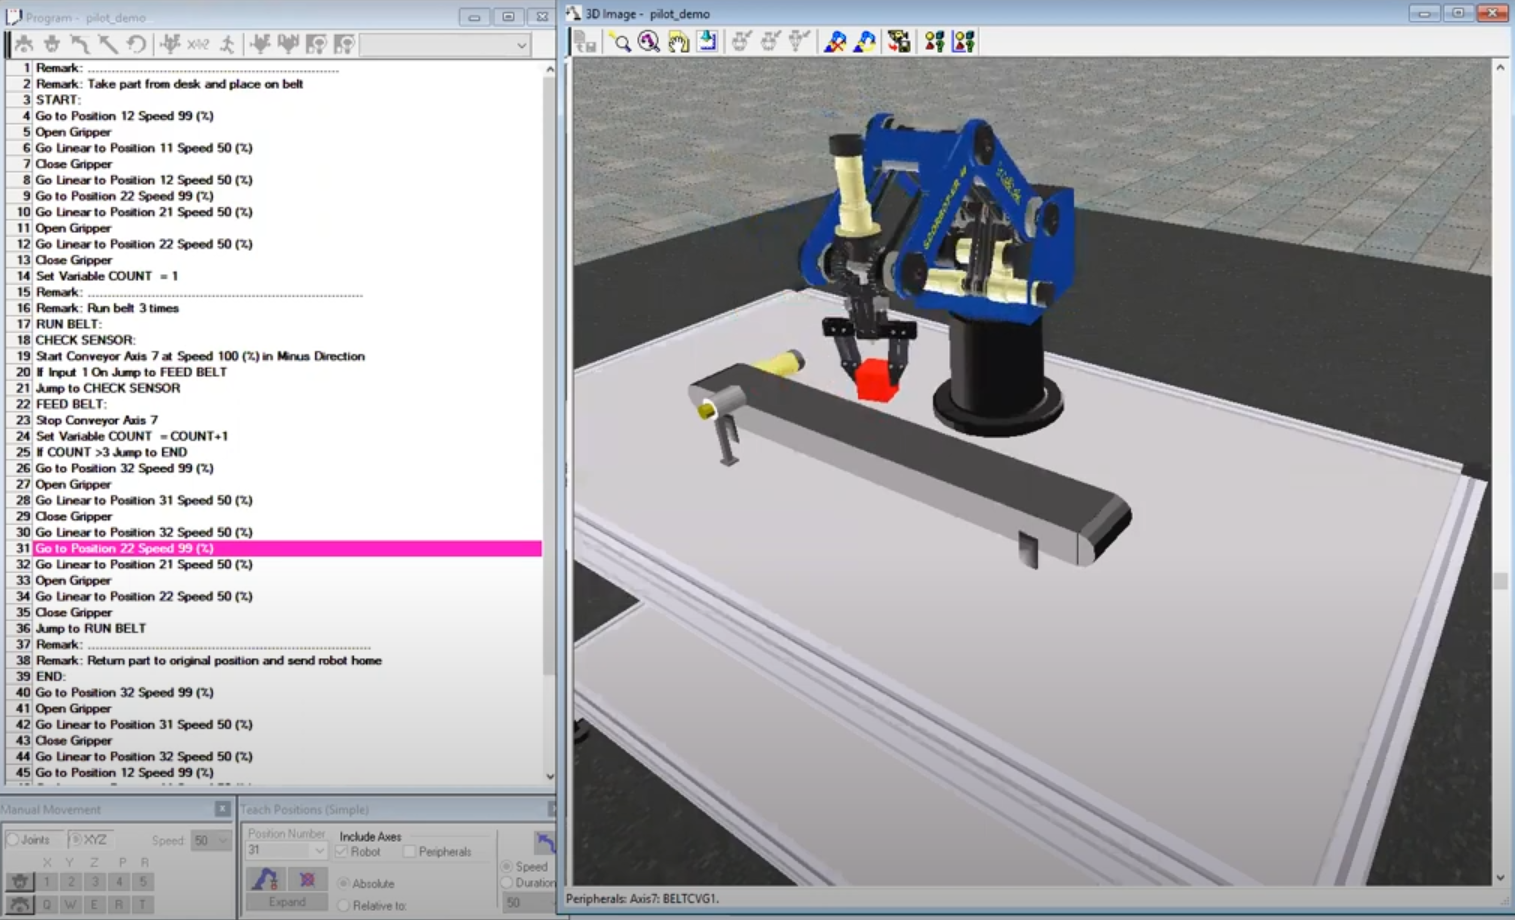
\includegraphics[width=13cm]{figures/modelo.png}
\caption{Diseño interfaz: Módulo Principal}
\label{fig:modelo}
\end{figure}
Estas son solo algunas ideas iniciales que pueden implementarse. La simulación no tiene límites, y el programa puede adaptarse para diversas finalidades, como la integración con la realidad virtual. Esto permitiría ampliar aún más las posibilidades de aprendizaje y entrenamiento, ofreciendo una experiencia inmersiva que podría abarcar desde el manejo básico de los brazos robóticos hasta aplicaciones más avanzadas en entornos simulados. Además, se podría explorar la opción de incorporar características de interactividad, permitiendo a los usuarios realizar prácticas y experimentos virtuales para consolidar sus conocimientos de manera práctica y segura. La flexibilidad del programa ofrece un amplio espectro de oportunidades para su expansión y adaptación a diferentes necesidades y contextos.
\chapter{Conclusiones} A lo largo de este proyecto, he podido comprender la importancia fundamental de mejorar la educación a través de la simulación \cite{Simulacion}. Aunque la simulación no puede replicar completamente la experiencia real, he observado que puede acercarse lo suficiente como para tener un impacto significativo en el proceso de aprendizaje. La capacidad de crear situaciones virtualmente similares a la realidad resulta especialmente relevante para eliminar barreras educativas, proporcionando alternativas accesibles y asequibles para personas con diversas limitaciones, como problemas de movilidad, foto-sensibilidad, discapacidad y otros obstáculos.

El enfoque de la simulación va más allá de simplemente recrear situaciones en un entorno virtual. Su verdadero potencial radica en la creación de un ambiente inclusivo donde todos puedan acceder a oportunidades educativas de manera efectiva, independientemente de sus capacidades físicas o cognitivas. Al adoptar esta herramienta en el ámbito educativo, se abren puertas para aquellas personas que, de otro modo, enfrentarían dificultades para participar en experiencias de aprendizaje costosas o restringidas.

En resumen, la simulación en la educación tiene el poder de promover una sociedad más equitativa e inclusiva, permitiendo que cada individuo alcance su máximo potencial. Aunque es un campo en desarrollo, espero que esta tesis inspire a educadores, instituciones académicas y desarrolladores tecnológicos a utilizar la simulación como una herramienta transformadora en la búsqueda de una educación para todos, sin barreras ni limitaciones. Al hacerlo, construiremos un futuro en el que la adquisición de conocimientos y habilidades sea una posibilidad accesible para cada persona, contribuyendo así al avance y prosperidad de la sociedad en su conjunto.

Por otra parte, reconozco que el proyecto resultó ser demasiado ambicioso para ser llevado a cabo por una sola persona en el tiempo limitado asignado. Es posible que con un equipo más extenso o con un plazo más amplio, el proyecto podría haberse ejecutado de manera exitosa. Este análisis subraya la importancia de contar con recursos adecuados y tiempo suficiente al abordar iniciativas de esta magnitud para garantizar resultados más satisfactorios.

\bibliography{bibliografia}

%\appendix
%\chapter{Propuesta de Tesis} \input{anexos/Anexo-01propuesta}
%\chapter{Ejemplos, datos, ...} \begin{lstlisting}[frame=single]
    using System.Collections;
    using System.Collections.Generic;
    using UnityEngine;
    using UnityEngine.UI;
    
    public class MovimientoJointsIX : MonoBehaviour
    {
        //Base
        private float velocidadRotacionBase = 80.0f; // Velocidad de rotación
        public KeyCode teclaRotacionPositivaBase = KeyCode.Q; // Tecla para la rotación en dirección positiva
        public KeyCode teclaRotacionNegativaBase = KeyCode.A; // Tecla para la rotación en dirección negativa
        public Transform Base; // Transform del objeto que se va a rotar
        private float LimitePositivoBase = 135.0f; // Angulo limite del objeto
        private float LimiteNegativoBase = -135.0f; // Angulo limite del objeto
        private float sumaRotacionBase = 0.0f; // Suma de la rotacion del objeto para su uso en limites
    
        //Shoulder
        private float velocidadRotacionShoulder = 69.0f; // Velocidad de rotación
        public KeyCode teclaRotacionPositivaShoulder = KeyCode.W; // Tecla para la rotación en dirección positiva
        public KeyCode teclaRotacionNegativaShoulder = KeyCode.S; // Tecla para la rotación en dirección negativa
        public Transform Shoulder; // Transform del objeto a rotar
        public Transform puntoFijoShoulder; // Transform del punto fijo alrededor del cual se realizará la rotación
        private float LimitePositivoShoulder = 72.5f; // Angulo limite del objeto
        private float LimiteNegativoShoulder = -72.5f; // Angulo limite del objeto
        private float sumaRotacionShoulder = 0.0f; // Suma de la rotacion del objeto para su uso en limites
    
        //Elbow
        private float velocidadRotacionElbow = 77.0f; // Velocidad de rotación
        public KeyCode teclaRotacionPositivaElbow = KeyCode.E; // Tecla para la rotación en dirección positiva
        public KeyCode teclaRotacionNegativaElbow = KeyCode.D; // Tecla para la rotación en dirección negativa
        public Transform Elbow; // Transform del objeto a rotar
        public Transform puntoFijoElbow; // Transform del punto fijo alrededor del cual se realizará la rotación
        private float LimitePositivoElbow = 105.0f; // Angulo limite del objeto
        private float LimiteNegativoElbow = -105.0f; // Angulo limite del objeto
        private float sumaRotacionElbow = 0.0f; // Suma de la rotacion del objeto para su uso en limites
    
        //Wrist
        private float velocidadRotacionWrist = 103.0f; // Velocidad de rotación
        public KeyCode teclaRotacionPositivaWrist = KeyCode.R; // Tecla para la rotación en dirección positiva
        public KeyCode teclaRotacionNegativaWrist = KeyCode.F; // Tecla para la rotación en dirección negativa
        public Transform Wrist; // Transform del objeto a rotar
        public Transform puntoFijoWrist; // Transform del punto fijo alrededor del cual se realizará la rotación
        private float LimitePositivoWrist= 98.0f; // Angulo limite del objeto
        private float LimiteNegativoWrist = -98.0f; // Angulo limite del objeto
        private float sumaRotacionWrist = 0.0f; // Suma de la rotacion del objeto para su uso en limites
    
        //EndEffector
        private float velocidadRotacionEndEffector = 175.0f; // Velocidad de rotación
        public KeyCode teclaRotacionPositivaEndEffector = KeyCode.T; // Tecla para la rotación en dirección positiva
        public KeyCode teclaRotacionNegativaEndEffector = KeyCode.G; // Tecla para la rotación en dirección negativa
        public Transform EndEffector; // Transform del objeto a rotar
        public Transform puntoFijoEndEffector; // Transform del punto fijo alrededor del cual se realizará la rotación
        private float LimitePositivoEndEffector = 368.5f; // Angulo limite del objeto
        private float LimiteNegativoEndEffector = -368.5f; // Angulo limite del objeto
        private float sumaRotacionEndEffector = 0.0f; // Suma de la rotacion del objeto para su uso en limites
    
        //Botonera
        private string nombreObjeto = "";
        private bool positivoboton = false;
        private bool negativoboton = false;
        private bool positivobotonZ = false;
        private bool negativobotonZ = false;
    
        private bool isControlPressed = false;
        private bool isAltPressed = false;
    
        private bool EmpezarGuardar = false;
        private bool TerminarGuardar = false;
        private bool EmpezarMover = false;
        private bool TerminarMover = false;
        private int NumeroUsar = -1;
    
        private Dictionary<int, float> GuardarBase = new Dictionary<int, float>();
        private Dictionary<int, float> GuardarShoulder = new Dictionary<int, float>();
        private Dictionary<int, float> GuardarElbow = new Dictionary<int, float>();
        private Dictionary<int, float> GuardarWrist = new Dictionary<int, float>();
        private Dictionary<int, float> GuardarEndEffector = new Dictionary<int, float>();
    
        private void Start()
        {
            GuardarBase.Add(0, 0f);
            GuardarShoulder.Add(0,0f);
            GuardarElbow.Add(0,0f);
            GuardarWrist.Add(0,0f);
            GuardarEndEffector.Add(0,0f);
        }
    
        private void Update()
        {
            Movimiento(Base, teclaRotacionPositivaBase, teclaRotacionNegativaBase, velocidadRotacionBase, LimitePositivoBase, LimiteNegativoBase, Base, Base.up, ref sumaRotacionBase);
            Movimiento(Shoulder, teclaRotacionPositivaShoulder, teclaRotacionNegativaShoulder, velocidadRotacionShoulder, LimitePositivoShoulder, LimiteNegativoShoulder, puntoFijoShoulder, puntoFijoShoulder.forward, ref sumaRotacionShoulder);
            Movimiento(Elbow, teclaRotacionPositivaElbow, teclaRotacionNegativaElbow, velocidadRotacionElbow, LimitePositivoElbow, LimiteNegativoElbow, puntoFijoElbow, puntoFijoElbow.forward, ref sumaRotacionElbow);
            Movimiento(Wrist, teclaRotacionPositivaWrist, teclaRotacionNegativaWrist, velocidadRotacionWrist, LimitePositivoWrist, LimiteNegativoWrist, puntoFijoWrist, Wrist.forward, ref sumaRotacionWrist);
            Movimiento(EndEffector, teclaRotacionPositivaEndEffector, teclaRotacionNegativaEndEffector, velocidadRotacionEndEffector, LimitePositivoEndEffector, LimiteNegativoEndEffector, puntoFijoEndEffector, EndEffector.right, ref sumaRotacionEndEffector);
            MovimientoBoton(nombreObjeto);
            Guardar();
            Usar();
            GuardarBoton();
            UsarBoton();
            MoverEje();
            MoverEjeBoton();
            
        }
     
        private void Movimiento(Transform objeto, KeyCode TeclaPositiva, KeyCode TeclaNegativa, float VelocidadRotacion, float anguloLimitePositivo, float anguloLimiteNegativo, Transform puntoFijo, Vector3 direccion, ref float Suma)
        {
            
            // Obtener la dirección de rotación basada en las teclas presionadas
            float direccionRotacion = 0.0f;
    
            if (Input.GetKey(TeclaPositiva))
            {
                direccionRotacion = 1.0f;
            }
            else if (Input.GetKey(TeclaNegativa))
            {
                direccionRotacion = -1.0f;
            }
    
            // Verificar si no se están presionando teclas de rotación
            if (direccionRotacion == 0.0f)
            {
                return;
            }
            // Calcular el ángulo de rotación
            float anguloRotacion = direccionRotacion * VelocidadRotacion * Time.deltaTime;
            
            // Calcular el ángulo de rotación limitado
            float anguloRotacionLimitado = Mathf.Clamp(Suma, anguloLimiteNegativo, anguloLimitePositivo);
            if(anguloRotacionLimitado == anguloLimiteNegativo && direccionRotacion < 0)
            {
                anguloRotacion = 0.0f;
            }
    
            if(anguloRotacionLimitado == anguloLimitePositivo && direccionRotacion > 0)
            {
                anguloRotacion = 0.0f;
            }
            // Realizar la rotación alrededor del punto fijo
            objeto.RotateAround(puntoFijo.position, direccion, anguloRotacion);
            Suma += anguloRotacion;
            Suma = Mathf.Clamp(Suma, anguloLimiteNegativo, anguloLimitePositivo);
        }
    
        private void MovimientoBoton(string nombre)
        {
            
            // Obtener la dirección de rotación basada en las teclas presionadas
            float direccionRotacionboton = 0.0f;
    
            if (positivoboton)
            {
                direccionRotacionboton = 1.0f;
            }
            if (negativoboton)
            {
                direccionRotacionboton = -1.0f;
            }
    
            // Verificar si no se están presionando teclas de rotación
            if (direccionRotacionboton == 0.0f)
            {
                return;
            }
            float Sumar = 0;
            Vector3 direccion = Vector3.up;
            float anguloLimitePositivo = 0;
            float anguloLimiteNegativo = 0;
            float VelocidadRotacion = 0;
            Transform puntoFijo = Base;
            Transform objeto = Base;
    
            if (nombre == "Base")
            {
                Sumar = sumaRotacionBase;
                direccion = Base.up;
                anguloLimitePositivo = LimitePositivoBase;
                anguloLimiteNegativo = LimiteNegativoBase;
                VelocidadRotacion = velocidadRotacionBase;
                puntoFijo = Base;
                objeto = Base;
            }
    
            if (nombre == "Shoulder")
            {
                Sumar = sumaRotacionShoulder;
                direccion = puntoFijoShoulder.forward;
                anguloLimitePositivo = LimitePositivoShoulder;
                anguloLimiteNegativo = LimiteNegativoShoulder;
                VelocidadRotacion = velocidadRotacionShoulder;
                puntoFijo = puntoFijoShoulder;
                objeto = Shoulder;
            }
    
            if (nombre == "Elbow")
            {
                Sumar = sumaRotacionElbow;
                direccion = puntoFijoElbow.forward;
                anguloLimitePositivo = LimitePositivoElbow;
                anguloLimiteNegativo = LimiteNegativoElbow;
                VelocidadRotacion = velocidadRotacionElbow;
                puntoFijo = puntoFijoElbow;
                objeto = Elbow;
            }
    
            if (nombre == "Wrist")
            {
                Sumar = sumaRotacionWrist;
                direccion = Wrist.up;
                anguloLimitePositivo = LimitePositivoWrist;
                anguloLimiteNegativo = LimiteNegativoWrist;
                VelocidadRotacion = velocidadRotacionWrist;
                puntoFijo = Wrist;
                objeto = Wrist;
            }
    
            if (nombre == "EndEffector")
            {
                Sumar = sumaRotacionEndEffector;
                direccion = EndEffector.up;
                anguloLimitePositivo = LimitePositivoEndEffector;
                anguloLimiteNegativo = LimiteNegativoEndEffector;
                VelocidadRotacion = velocidadRotacionEndEffector;
                puntoFijo = EndEffector;
                objeto = EndEffector;
            }
            
            // Calcular el ángulo de rotación
            float anguloRotacion = direccionRotacionboton * VelocidadRotacion * Time.deltaTime;
            
            // Calcular el ángulo de rotación limitado
            float anguloRotacionLimitado = Mathf.Clamp(Sumar, anguloLimiteNegativo, anguloLimitePositivo);
            if(anguloRotacionLimitado == anguloLimiteNegativo && direccionRotacionboton < 0)
            {
                anguloRotacion = 0.0f;
            }
    
            if(anguloRotacionLimitado == anguloLimitePositivo && direccionRotacionboton > 0)
            {
                anguloRotacion = 0.0f;
            }
            // Realizar la rotación alrededor del punto fijo
            objeto.RotateAround(puntoFijo.position, direccion, anguloRotacion);
            Sumar += anguloRotacion;
            Sumar = Mathf.Clamp(Sumar, anguloLimiteNegativo, anguloLimitePositivo);
    
            if (nombre == "Base")
            {
                sumaRotacionBase = Sumar;
            }
    
            if (nombre == "Shoulder")
            {
                sumaRotacionShoulder = Sumar;
            }
    
            if (nombre == "Elbow")
            {
                sumaRotacionElbow = Sumar;
            }
    
            if (nombre == "Wrist")
            {
                sumaRotacionWrist = Sumar;
            }
            if (nombre == "EndEffector")
            {
                sumaRotacionEndEffector = Sumar;
            }
            
        }
    
        public void PointerUpPositivo(string nombre)
        {
            nombreObjeto = nombre;
            positivoboton = false;
        }
    
        public void PointerDownPositivo(string nombre)
        {
            nombreObjeto = nombre;
            positivoboton = true;
            
        }
    
        public void PointerUpNegativo(string nombre)
        {
            nombreObjeto = nombre;
            negativoboton = false;
        }
    
        public void PointerDownNegativo(string nombre)
        {
            nombreObjeto = nombre;
            negativoboton = true;
        }
    
        public void PointerUpPositivoZ()
        {
            if(!EmpezarGuardar && !EmpezarMover)
            {
                positivobotonZ = false;
            }
        }
    
        public void PointerDownPositivoZ()
        {
            if(!EmpezarGuardar && !EmpezarMover)
            {
                positivobotonZ = true;
            }
        }
    
        public void PointerUpNegativoZ()
        {
            if(!EmpezarGuardar && !EmpezarMover)
            {
                negativobotonZ = false;
            }
        }
    
        public void PointerDownNegativoZ()
        {
            if(!EmpezarGuardar && !EmpezarMover)
            {
                negativobotonZ = true;
            }
        }
    
        private void Guardar()
        {
            // Verificar si se presionó la tecla de control (Ctrl)
            if (Input.GetKey(KeyCode.LeftControl) || Input.GetKey(KeyCode.RightControl))
            {
                isControlPressed = true;
            }
    
            // Verificar si está habilitado el registro de teclas
            if (isControlPressed)
            {
                // Verificar las teclas numéricas del 1 al 9
                for (int i = 1; i <= 9; i++)
                {
                    if (Input.GetKey(i.ToString()))
                    {
                        SaveInformation(i);
                        isControlPressed = false;
                    }
                }
            }
        }
    
        private void GuardarBoton()
        {
            // Verificar si se presionó el boton
            if (EmpezarGuardar)
            {
                // Verificar si se habilita el guardado
                if (TerminarGuardar)
                {
                    SaveInformation(NumeroUsar);
                    TerminarGuardar = false;
                    EmpezarGuardar = false;
                    NumeroUsar = -1;
                }
            }     
        }
    
        private void Usar()
        {
            // Verificar si se presionó la tecla de control (Ctrl)
            if (Input.GetKey(KeyCode.LeftAlt) || Input.GetKey(KeyCode.RightAlt))
            {
                isAltPressed = true;
            }
    
            // Verificar si está habilitado el registro de teclas
            if (isAltPressed)
            {
                // Verificar las teclas numéricas del 0 al 9
                for (int i = 0; i <= 9; i++)
                {
                    if (Input.GetKey(i.ToString()))
                    {
                        GetInformation(i);
                        isAltPressed = false;
                    }
                }
            }
        }
    
        private void UsarBoton()
        {
            // Verificar si se presionó el boton
            if (EmpezarMover)
            {
                // Verificar si se habilita el guardado
                if (TerminarMover)
                {
                    GetInformation(NumeroUsar);
                    TerminarMover = false;
                    EmpezarMover = false;
                    NumeroUsar = -1;
                }
            }
        }
    
        private void SaveInformation(int i)
        {
            if (GuardarBase.ContainsKey(i))
            {
                GuardarBase[i] = sumaRotacionBase;
            }
            else
            {
                GuardarBase.Add(i,sumaRotacionBase);
            }
    
            if (GuardarShoulder.ContainsKey(i))
            {
                GuardarShoulder[i] = sumaRotacionShoulder;
            }
            else
            {
                GuardarShoulder.Add(i, sumaRotacionShoulder);
            }
    
            if (GuardarElbow.ContainsKey(i))
            {
                GuardarElbow[i] = sumaRotacionElbow;
            }
            else
            {
                GuardarElbow.Add(i, sumaRotacionElbow);
            }
    
            if (GuardarWrist.ContainsKey(i))
            {
                GuardarWrist[i] = sumaRotacionWrist;
            }
            else
            {
                GuardarWrist.Add(i, sumaRotacionWrist);
            }
    
            if (GuardarEndEffector.ContainsKey(i))
            {
                GuardarEndEffector[i] = sumaRotacionEndEffector;
            }
            else
            {
                GuardarEndEffector.Add(i, sumaRotacionEndEffector);
            }
        }
    
        private void GetInformation(int i)
        {
            if (GuardarBase.ContainsKey(i))
            {
                float value = GuardarBase[i];
                Debug.Log("Base "+ i + " = " + value);
                //MoverGuardado(value,sumaRotacionBase,Base,Base,LimiteNegativoBase,LimitePositivoBase,velocidadRotacionBase,-Base.up);
            }
            else
            {
                Debug.Log("no existe");
            }
    
            if (GuardarShoulder.ContainsKey(i))
            {
                float value = GuardarShoulder[i];
                Debug.Log("Shoulder "+ i + " = " + value);
            }
            else
            {
                Debug.Log("no existe");
            }
    
            if (GuardarElbow.ContainsKey(i))
            {
                float value = GuardarElbow[i];
                Debug.Log("Elbow "+ i + " = " + value);
            }
            else
            {
                Debug.Log("no existe");
            }
    
            if (GuardarWrist.ContainsKey(i))
            {
                float value = GuardarWrist[i];
                Debug.Log("Wrist "+ i + " = " + value);
            }
            else
            {
                Debug.Log("no existe");
            }
    
            if (GuardarEndEffector.ContainsKey(i))
            {
                float value = GuardarEndEffector[i];
                Debug.Log("EndEffector "+ i + " = " + value);
            }
            else
            {
                Debug.Log("no existe");
            }
        }
    
        public void EmpezarAGuardar()
        {
            EmpezarGuardar = true;
        }
    
        public void NumeroAUsar(int i)
        {
            if(EmpezarGuardar || EmpezarMover)
            {
                NumeroUsar = i;
            }
        }
    
        public void TerminarAGuardar()
        {
            if(0 < NumeroUsar && NumeroUsar < 10)
            {
                if(EmpezarGuardar)
                {
                    TerminarGuardar = true;
                }
            }
        }
    
        public void EmpezarAMover()
        {
            EmpezarMover = true;
        }
    
        public void TerminarAMover()
        {
            if(-1 < NumeroUsar && NumeroUsar < 10)
            {
                if(EmpezarMover)
                {
                    TerminarMover = true;
                }
                
            }
        }
    
        private void MoverEje()
        {
            float movimiento = 0f;
    
            // Verifica si se presiona la tecla positiva
            if (Input.GetKey(KeyCode.Alpha1))
            {
                movimiento = 1f;
            }
    
            // Verifica si se presiona la tecla negativa
            if (Input.GetKey(KeyCode.Alpha6))
            {
                movimiento = -1f;
            }
    
            // Mueve el objeto en el eje Y (o el eje que desees) según el valor de movimiento
            transform.Translate(Vector3.right * movimiento * 5f * Time.deltaTime);
        }
    
        private void MoverEjeBoton()
        {
            float movimiento = 0f;
    
            if (positivobotonZ)
            {
                movimiento = 1.0f;
            }
            if (negativobotonZ)
            {
                movimiento = -1.0f;
            }
    
            // Mueve el objeto en el eje Y (o el eje que desees) según el valor de movimiento
            transform.Translate(Vector3.right * movimiento * 5f * Time.deltaTime);
        }
    
        private void MoverGuardado(float valor, float Suma, Transform puntoFijo, Transform objeto, float anguloLimiteNegativo, float anguloLimitePositivo, float VelocidadRotacion, Vector3 direccion)
        {
            
            float direccionRotacion = 0.0f;
    
            if (Suma < valor)
            {
                direccionRotacion = 1.0f;
            }
            else if (Suma > valor)
            {
                direccionRotacion = -1.0f;
            }
    
            if (direccionRotacion == 0.0f)
            {
                return;
            }
            // Calcular el ángulo de rotación
            
            // Realizar la rotación alrededor del punto fijo
            while(Suma != valor)
            {
                float anguloRotacion = direccionRotacion * VelocidadRotacion * Time.deltaTime;
                objeto.RotateAround(puntoFijo.position, direccion, anguloRotacion);
                Suma += anguloRotacion;
                if(direccionRotacion == 1.0f)
                {
                    Suma = Mathf.Clamp(Suma, anguloLimiteNegativo, valor);
                }
                else
                {
                    Suma = Mathf.Clamp(Suma, valor, anguloLimitePositivo);
                }
                
            }
            
        }
    }
\end{lstlisting}
%\chapter{Manual de ususario} \begin{lstlisting}[frame=single]
    using System.Collections;
    using System.Collections.Generic;
    using UnityEngine;
    using UnityEngine.UI;

    public class PantallaCompleta : MonoBehaviour
    {
        
        public Toggle toggle;
        public Dropdown resolucionesDropdown;
        Resolution[] resoluciones;
        
        void Start()
        {
            if (Screen.fullScreen)
            {
                toggle.isOn = true;
            }
            else
            {
                toggle.isOn = false;
            }

            RevisarResolucion();
        }

        // Update is called once per frame
        void Update()
        {
            
        }
        
        public void ActivarPantallaCompleta(bool pantallaCompleta)
        {
            Screen.fullScreen = pantallaCompleta;
        }

        public void RevisarResolucion()
        {
            resoluciones = Screen.resolutions;
            resolucionesDropdown.ClearOptions();
            List<string> opciones = new List<string>();
            int resolucionActual = 0;
            
            for (int i = 0; i < resoluciones.Length; i++)
            {
                string opcion = resoluciones[i].width + " x " + resoluciones[i].height;
                opciones.Add(opcion);
                
                if(Screen.fullScreen && resoluciones[i].width == Screen.currentResolution.width && resoluciones[i].height == Screen.currentResolution.height)
                {
                    resolucionActual = i;
                }
            }
            resolucionesDropdown.AddOptions(opciones);
            resolucionesDropdown.value = resolucionActual;
            resolucionesDropdown.RefreshShownValue();
            resolucionesDropdown.value = PlayerPrefs.GetInt("numeroResolucion",0);
        }
        
        public void CambiarResolucion(int indiceResolucion)
        {
            PlayerPrefs.SetInt("numeroResolucion",resolucionesDropdown.value);
            Resolution resolucion = resoluciones[indiceResolucion];
            Screen.SetResolution(resolucion.width, resolucion.height, Screen.fullScreen);
        }
    }
\end{lstlisting}

\end{document}
